\documentclass[12pt,twoside]{book}
\usepackage[utf8]{inputenc}
\usepackage{amsmath}
\usepackage{amsfonts}
\usepackage{amssymb}
\usepackage{makeidx}
\usepackage{graphicx}

\usepackage{babel}
\newcommand{\ESP}[1]{\foreignlanguage{spanish}{#1}}
%\usepackage[left=4cm,right=3cm,top=3.5cm,bottom=3.5cm]{geometry}
\usepackage{cite}

\let\tmp\oddsidemargin
\let\oddsidemargin\evensidemargin
\let\evensidemargin\tmp
\reversemarginpar


\usepackage{lmodern} %fuentes
%\usepackage[T1]{fontenc} %fuentes
%\usepackage[spanish]{babel} %idoma
\usepackage{caption, subcaption} %figuras
%\usepackage{graphicx}
\usepackage{array}
%\usepackage{bachelorstitlepageUNAM}

\usepackage{pdfpages}

\usepackage{tikz}
\usetikzlibrary{spy}

%\author{Jos\'e Antonio Garc\'ia Hern\'andez}
%\title{The profile of non-standard cosmic strings}
%\faculty{Instituto de Ciencias Nucleares}
%\degree{MAESTR\'IA EN CIENCIAS F\'ISICAS}
%\supervisor{Dr. Wolfgang Peter Bietenholz}
%\cityandyear{Ciudad Universitaria, Cd. Mx., 2022}
%\logouni{Escudo-UNAM}
%\logofac{logoicn.png}

%\date{}

%calligraphic style. Used to represent the C in the loop space in chapter 1
\usepackage[scr=rsfso,frak=euler]{mathalfa}


\usepackage{hyphenat}
\hyphenation{cho-le-ster-ic}
%
\usepackage{amsthm}
\theoremstyle{definition}
\newtheorem{definition}{Definition}[section]


\allowdisplaybreaks

%CAncel terms
\usepackage{cancel}

% References

%\usepackage[backend=biber,sorting=none]{biblatex}

\usepackage{natbib}
% Package for enhancing apalike and other default bibliographies
\bibliographystyle{unsrt}
% Just a bibliographystyle
\usepackage{url}
% Package for including urls in bibliography

\usepackage{fancyhdr}
\lhead{}
% Package for setting the header and footinoter of pages
%\pagestyle{fancy}



\usepackage{epstopdf}
% package for including eps figures and convert them to pdf and present them

\graphicspath{{./images/}}
% Folder where all the pictures are saved

\usepackage{setspace}
\onehalfspacing
% Package and command to set the spacing in the document
\linespread{1.5}

%\setlength{\marginparwidth}{0pt}

\usepackage[breaklinks=true,bookmarks=true,bookmarksopen=true,colorlinks=true,linkcolor=blue,citecolor=red,pdfhighlight=/P]{hyperref}
% For including Hyperlinks in the document

%\usepackage[a4paper,top=1.5in,bottom=1.5in,left=2in,right=1.5in]{geometry}
% Package for setting up the shape of the page

\pagestyle{fancy}
% A predefined page style in fancyhdr package

\begin{document}
%	\begin{titlepage}
		\setlength{\parindent}{0pt} \setlength{\parskip}{0pt}
	
		\begin{center}
			%\vfill 
			
			\begin{minipage}{\textwidth}
				
				\newcolumntype{V}{>{\centering\arraybackslash} m{.17\textwidth} }
				\newcolumntype{C}{>{\centering\arraybackslash} m{.56\textwidth} }
				
				\begin{center}
					
\includegraphics[width=4cm]{Escudo-UNAM.pdf}	
				\end{center} 	
				\begin{center}
					\Large\textbf{\sc Universidad Nacional Aut\'onoma de M\'exico}
				\end{center} 
				
			\end{minipage}
				
			\vfill
			
			\begin{minipage}{0.7\textwidth}
				\begin{center}
					\large \sc Programa de Posgrado en Ciencias Fisicas
				\end{center}
			\end{minipage}
			% 
			\begin{center}
				
				%\vfill
				%\medskip \rule{.9\textwidth}{2pt}
				%\vfill
				\Huge \textbf{\sc The profile of non-standard cosmic strings}
				%{\Large \bfseries  \title   }
				
				%\medskip \rule{.9\textwidth}{2pt}
			\end{center}		
			\begin{center}
				\vspace*{0.3cm}
				{\large T E S I S}\\
				\vspace*{0.3cm}
				\sc que para optar por el grado de \\ \bigskip
				{\Large {\sc Maestro en ciencias físicas}} \\ \bigskip
				
				%PRESENTA:\\ \medskip
				\begin{center}
					\sc PRESENTA: \\
					\Large José Antonio García Hernández
				\end{center}
				
				%\bigskip
				
				Tutor Principal: \\
				Wolfgang Peter Bietenholz\\
				%Coadvisors
				%\emph{Coasesores:}
				%\coadvisor1 \\ \coadvisor2 \\ \coadvisor3 
			\end{center}
			
			%\vfill
			
			\begin{center}
				{México, CDMX. Abril 2022}\\
			\end{center}
			\cleardoublepage
		\end{center}
	\end{titlepage}
%\frontmatter
%\includepdf[pages={1}]{/home/jose/Documents/Maestria/thesis/chapters/build/portada.pdf}
%\maketitle
\includepdf[pages=-]{./build/titlepage.pdf}

%	\begin{titlepage}
%		\setlength{\parindent}{0pt} \setlength{\parskip}{0pt}
%	
%		\begin{center}
%			\vfill 
%			
%			\begin{minipage}{\textwidth}
%				
%				\newcolumntype{V}{>{\centering\arraybackslash} m{.17\textwidth} }
%				\newcolumntype{C}{>{\centering\arraybackslash} m{.56\textwidth} }
%				
%				\begin{center}
%					
\includegraphics[width=4cm]{Escudo-UNAM.pdf}	
%				\end{center} 	
%				\begin{center}
%					\textbf{\large{Universidad Nacional Aut\'onoma de M\'exico}}
%				\end{center} 
%				
%			\end{minipage}
%				
%			\vfill
%			
%			\begin{minipage}{\textwidth}
%				\begin{center}
%					\large \sc Programa de Posgrado en Ciencias Físicas
%				\end{center}
%			\end{minipage}
%			 
%			\begin{center}
%				
%				%\vfill
%				\medskip \rule{.9\textwidth}{2pt}
%				\vfill
%				\Huge \textbf{\sc The profile of non-standard cosmic strings}
%				{\Large \bfseries  \title   }
%				
%				%\medskip \rule{.9\textwidth}{2pt}
%			\end{center}		
%			\begin{center}
%				\vspace*{0.3cm}
%				{\large \textbf{T E S I S}}\\
%				\vspace*{0.3cm}
%				\sc que para optar por el grado de \\ \bigskip
%				{\large {\sc Maestro en ciencias físicas}} \\ \bigskip
%				
%				%PRESENTA:\\ \medskip
%				\begin{center}
%					\sc \textbf{PRESENTA} \\
%					\Large José Antonio García Hernández
%				\end{center}				
%				Tutor Principal: \\
%				Wolfgang Bietenholz, ICN\\
%				Coadvisors
%				{Comité Tutor:}\\
%				Dr. José Alejandro Ayala Mercado, ICN\\
%				Dr. Eduardo Peinado Rodríguez, IF
%				
%			\end{center}
%			
%			%\vfill
%			
%			\begin{center}
%				{México, CDMX.  2023}\\
%			\end{center}
%			\cleardoublepage
%		\end{center}
%	\end{titlepage}
%\frontmatter
%\includepdf[pages={1}]{/home/jose/Documents/Maestria/thesis/chapters/build/portada.pdf}
%\maketitle

%\documentclass[12pt,a4paper,twoside]{book}
\usepackage[utf8]{inputenc}
\usepackage[english]{babel}
\usepackage{amsmath}
\usepackage{amsfonts}
\usepackage{amssymb}
\usepackage{graphicx}
\let\tmp\oddsidemargin
\let\oddsidemargin\evensidemargin
\let\evensidemargin\tmp
\reversemarginpar

\author{José Antonio García-Hernández}
\linespread{1.5}
\begin{document}

\begin{titlepage}
\begin{center}

		
\includegraphics[width=4.4cm]{Escudo-UNAM.pdf}	\\
		\vspace{0.3cm}	
		\sc			
		\textbf{ UNIVERSIDAD NACIONAL AUT\'ONOMA DE M\'EXICO} \\
		\small Posgrado en Ciencias F\'isicas \\
		\vspace*{0.3cm}
		\begin{tabular}{c}
		\hline\hline
\vspace{-5mm}\\
		\Huge{\sc{The profile of non-standard}}\\
		\Huge{\sc{cosmic strings}}\\\hline\hline
		\end{tabular}\\
		\vspace*{0.3cm}
		\normalsize
		\textbf{TESIS}\\
		Que para optar por el grado de:\\
Maestro en Ciencias (F\'isica)\\
\vspace*{0.3cm}
\textbf{PRESENTA}\\
{\large Jos\'e Antonio Garc\'ia Hern\'andez}\\
\vspace*{0.3cm}
\textbf{TUTOR PRINCIPAL}\\
Dr.\ Wolfgang Peter Bietenholz\\
Instituto de Ciencias Nucleares\\
\vspace*{0.3cm}
\textbf{COMIT\'E TUTOR}\\
Dr.\ Eduardo Peinado Rodríguez\\
Instituto de F\'isica\\
Dr.\ Jos\'e Alejandro Ayala Mercado \\
Instituto de Ciencias Nucleares\\

	\vspace*{0.3cm}	
		{Ciudad Universitaria, Cd. de M\'exico, Abril 2023}
		
\end{center}

\end{titlepage}

\end{document}

\chapter*{Acknowledgments}
First and foremost I would like to thank my advisor Dr.\ Bietenholz, without him this thesis could never have been done. I am really grateful for his  insightful comments, and patience over these years under his guidance.

I acknowledge financial support from \ESP{\textit{programa de becas nacionales}} of the CONACYT and an additional scholarship from the project DGAPA-PAPIIT IG100322 ``\textit{Materia fuertemente acoplada en condiciones extremas con el MPD-NICA}''. 

In addition, I would like to acknowledge Víctor Muñoz, who collaborated in the project and confirmed the equations of motion and the co-axial string solutions.

%I am really indebted to CONACYT, my advisor Dr.\ Wolfgang Bietenholz and Pixi Payasita for their support...

\chapter*{Resumen}
\ESP{Se asume que a través del llamado \textit{mecanismo de Kibble} en el universo temprano pudieron haberse formado defectos topológicos. En esta tesis discutimos un modelo más allá del Modelo Estándar que permite un tipo de defectos topológicos llamado \textit{cuerda cósmica}. Para estudiar soluciones de cuerdas cósmicas, primero promovemos la simetría global U$(1)_{B-L}$ a una simetría local y agregamos un nuevo acoplamiento de norma. La cancelación de las anomalías de norma se logra agregando un neutrino derecho a cada generaci\'on de leptones. Además, se agrega un nuevo campo de Higgs para dar masa al neutrino derecho. Finalmente, estudiamos las ecuaciones de movimiento de los dos campos de Higgs y el campo de norma, con el fin de obtener los perfiles de las cuerdas cósmicas. Particularmente, descubrimos un tipo de soluciones a las que llamamos  de cuerdas cósmicas coaxiales. Adicionalmente, obtuvimos que la tensión de las cuerdas es del orden de $10^{19}\ \text{GeV}^{2}$ y su acoplamiento gravitacional $\sim 10^{-30}$ el cual está por debajo de las constricciones obtenidas por la colaboración LIGO.}

\chapter*{Abstract}
It is generally assumed that through the so-called \textit{Kibble mechanism} objects called topological defects could have formed in the early universe. In this thesis we discuss a model beyond the Standard Model that permits a type of topological defects called \textit{cosmic strings}. In order to study cosmic string solutions, we first promote the global symmetry U$(1)_{B-L}$ to a local symmetry and add a new gauge coupling. The cancellation of gauge anomalies is achieved by adding a right-handed neutrino to each lepton generation. More\-over, a new Higgs field is added in order to give mass to the right-handed neutrino.  
Finally, we study the field equations of motion of the two Higgs fields and the gauge field, in order to obtain the profiles of the cosmic strings. We compute this profile numerically and discuss their physical meaning. Particularly we found a type of solutions that we call coaxial cosmic strings.  In addition, we obtained the string tension which is of the order of $10^{19}\,\text{GeV}^2$ and its gravitational coupling $\sim 10^{-30}$ which is below from the constrictions obtained by the LIGO collaboration.
\tableofcontents

\chapter{Introduction}\label{chap:intro}
In recent years, the study of topological defects is becoming of great interest in modern physics. In field theories, topological defects could be found as solitonic stable solutions of the classical field equations.

In general, a topological defect can be defined as a discontinuity in the order parameter space of the system. In condensed matter physics, there are several examples of topological defects, but in the physics of the early universe, they are still hypothetical. For instance, topological defects are a generic prediction in Grand Unified Theories.

It is generally assumed that in the early universe several phase transitions occurred, giving rise to topological defects by means of the Kibble mechanism \cite{Kibble1976,Kibble1980}. If they exist, we expect on average at least one topological defect per horizon volume.

An example of a topological defect forming in the early universe is the vortex line or \emph{cosmic string}. Cosmic strings are elongated concentrations of energy that are very thin, and can be considered effectively as 1-dimensional. They can be closed or open and very large, of the order of a cosmic horizon.

If cosmic strings exist, they can be of various types. For instance, they can be global strings, which emerge from a global symmetry, or local strings, which originate from a local symmetry. Global strings have the property that their tension is infinite. On the other hand, local strings have a finite tension. U(1) local strings are also known as Nielsen-Olesen strings, and have the property that their magnetic flux is quantized. 

In addition, there is another type of string called the superconducting string \cite{WITTEN1985557}. This type of string behaves like a superconducting wire, in which current can be carried by bosons or fermions.


Intense research of cosmic strings is being performed recently, in particular, some research like in Ref.\ \cite{PhysRevD.97.102002} aims to detect their gravitational waves signals, which set constraints to the tension of the string. Moreover, cosmic strings have a characteristic discontinuity effect in the CMB (Cosmic Microwave Background) temperature which could possibly be measured. Cosmic super\-strings, on the other hand can produce cosmic rays such as $\gamma$-rays.

Since they are very thin, of the order of 1 fm or even less, their dynamics  can be studied in the zero width limit as Nambu-Goto strings. 

They were once believed to be the seed for large structures such as galaxies, as reviewed in Ref.\ \cite{kibble1986}. However, measurements of the CMB power spectrum by COBE  (COsmic Background Explorer) and WMAP (the Wil\-kin\-son Microwave Anisotropy Probe) discarded the possibility of cosmic strings having an effect on the formation of large structures. These meas\-ure\-ments showed that the angular power spectrum has acoustic peaks that are not explained by cosmic strings, see Ref.\ \cite{pogo2006}. 

The importance of topological defects in the universe is that they would be directly observables as relics of the primordial fields in the early universe.

The objective of this thesis is to study numerically the profile of cosmic strings related to the local invariance of the symmetry $\text{U}(1)_{B-L}$. We are particularly interested in co-axial string solutions. Co-axial solutions are negative at low $r$, pass the $r$ axis, and then approach their positive boundary value at $r\to\infty$.

Throughout this thesis, we will work with natural units where $c=\hbar=k_B = 1$.

In Chapter 2, we present the mathematical background required, such as concepts in topology and group theory, and also give examples of topological defects in other branches of physics. In Chapter 3, we focus on cosmic strings, we study the solutions to global and local U(1) strings, and give a review of the research done to detect them. Chapter 4 is completely original, we describe cosmic strings solutions enabled by a scenario ``Beyond the Standard Model" (BSM) where we promote the global U$(1)_{B-L}$ symmetry to a local symmetry and we combine it with U$(1)_Y$ which leads to the group we call U$(1)_{Y'}$. In Chapter 5, we present solutions to the equations of motion for the fields and discuss the profile of local U$(1)_{Y'}$ cosmic strings within this BSM model. 




\chapter{Theoretical background}\label{chap:back}
In physics there exist mathematical structures known as topological defects that are singularities that cannot be removed without affecting the system at large scales.
Condensed matter systems provide many examples of the existence of topological defects. A particular case are vortex-like structures: at low temperatures, there are magnetic flux lines in type II superconductors and quantized vortex lines in superfluid $^{3}$He and $^4$He \cite{Zurek1985,Zurek1993,Zurek1996,bunkov,PhysRevLett.43.214,ancio2015}.

\section{Topological defects}\label{sec:topdef}
In order to define a topological defect, we first review some other definitions. Generally speaking, an \textit{order parameter} can be any quantity that is defined in a physical system, in space or spacetime, that distinguishes between ordered and disordered phases. It is zero when the system is in the disordered phase, and non-zero when it is in the ordered phase. The set of values that the order parameter can take is called the \textit{order parameter space} or \textit{order parameter manifold}.

A topological defect can be defined as a discontinuity in the order pa\-ram\-e\-ter space of a system. The definition suggests that an order parameter is related to changes of phases, spontaneous symmetry breaking, etc. Top\-o\-log\-i\-cal defects have the feature that they are extremely stable, meaning that no local rearrangement of the order parameter can remove them. 

The study of topological defects rely on homotopy theory. Homotopy theory deals with the use of continuous deformations that transform one object into another thus establishing their topological equivalence. A par\-tic\-u\-lar\-ly simple deformable object is a \textit{path} and if the path is closed it is called a \textit{loop}. In the following we give some useful definitions in topology. Sections \ref{sec:topdef} and  \ref{sec:examples} are based on Ref.\ \cite{mermin1979}. 

%Examples of ordered media are the spin models. An 'spin' is defined as a vector quantity of $n$ dimensions attached to every point a given region, usually spins are normalize to unity.


\subsection{Review of topology}\label{sec:revtop}
The study of topology in physics is important. In particular, the topology of the vacuum manifold $\mathcal{M}$ defines what topological defect can arise. %More specifically, the behavior of topological defects is studied by homotopy theory.

 
%\begin{definition}
%Two continuous maps between topological spaces $f: X\to Y$ and $g: X\to Y$ are \textbf{homotopic} if there exists a continuous function
%\begin{equation}
%	H: X\times[0,1]\to Y,
%\end{equation}
%such that
%\begin{equation}
%	H(x,0) = f(x), \ \ \ H(x,1) = g(x).
%\end{equation}
%\end{definition}
\begin{definition}[Topology]
Let the set $X\neq \emptyset$. A collection of subsets $\tau$ of $X$, called open sets, is said to be a \textit{topology} if they satisfy the following properties:
\begin{enumerate}
\item $X,\emptyset \in \tau$,
\item $U_1,\ U_2 \in \tau \Rightarrow U_1\cap U_2 \in \tau$,
\item $U_i \in \tau$, $\forall i\in I\Rightarrow$ $\bigcup_{i\in I} U_i \in \tau$, where $I$ is a set of indices.
\end{enumerate}
The pair $(X,\tau)$ is called a \textit{topological space}.
\end{definition}
The appeal of a topological space is that it is the most general space one can work with, in the sense that closeness can be defined by the definition above. The definition of path connectedness and the idea of loops can be used to describe the holes in a topological space.

\begin{definition}[Path]
Let $x_0,x_1\in X$. A \textit{path} $\gamma$ in $X$ from $x_0$ to $x_1$ is a continuous map
\begin{equation}
	\gamma: [0,1] \to X,
\end{equation}
with
\begin{equation}
	\gamma(0) = x_0, \ \ \ \gamma(1) = x_1.
\end{equation}
\end{definition}
We say that a topological space $X$ is \textit{path connected} if there exists a path connecting any two points $x_0,x_1\in X$.

\begin{definition}[Loop]
 A \textit{loop} in a topological space $X$ at the base point $x_0 \in X$ is a continuous map 
 \begin{equation}
	\gamma: [0,1] \to X,
\end{equation}
with
 \begin{equation}
 	\gamma(0) = \gamma(1) = x_0.
 \end{equation}
 Equivalently we can write  this map as
 \begin{equation}
 	\gamma : S^1 \to X,
 \end{equation}
 where $S^1$ is the 1-sphere.
 The space of all loops at $x_0\in X$ or \textit{loop space} at the base point $x_0\in X$ is denoted $\mathscr{C}_{x_0}(X)$.
\end{definition}
The loops defined above are also called 1-dimensional loops and can be generalized to higher dimensions. An $n$-th loop is a smooth map from the $n$-sphere to the topological space $\gamma : S^{n} \to X$.
\begin{definition}[Constant loop] The \textit{constant loop} $e$ at $x_0\in X$ is defined as
	\begin{equation}
		e(t) = x_0, \ \ \ 0\leq t \leq 1.
	\end{equation}
\end{definition}

\begin{definition}[Inverse loop]
Consider the loop $\gamma$ at $x_0\in X$. Its \textit{inverse loop} $\gamma^{-1}$ is defined as 
	\begin{equation}
		\gamma^{-1}(t) = \gamma(1-t), \ \ \ 0 \leq t \leq 1.
	\end{equation}
\end{definition}

\begin{definition}[Homotopic loops] Two loops $\gamma$ and $\gamma'$ at $x_0 \in X$ are \textit{homotopic loops} denoted $\gamma \sim \gamma'$, if there exists a continuous map
\begin{equation}
	H: [0,1]\times[0,1] \to X,
\end{equation}
such that
\begin{eqnarray}
	H(t,0) = \gamma(t), & & 0\leq t \leq 1, \nonumber \\ 
	H(t,1) = \gamma'(t), & & 0\leq t \leq 1,  \nonumber\\
	H(0,s) = H(1,s) = x_0, & & 0\leq s \leq 1. 
\end{eqnarray}
\end{definition}

The homotopy of loops, and more generally of paths, forms an equivalence relation meaning that they satisfy the properties of \textit{symmetry}, \textit{reflexivity} and \textit{transitivity}. %Clearly, a loop $\gamma$ is homotopic to itself, satisfying reflexivity, that is $\gamma\sim\gamma$
Reflexivity means that an element $a$ of an equivalence relation is equivalent to itself, that is, $a\sim a$. If $a$ and $b$ are elements of the equivalence relation, symmetry implies $a\sim b$ if and only if $b\sim a$. Transitivity means that that if $a\sim b$ and $b\sim c$ then $a\sim c$.


We denote an equivalence class as $[\gamma] = \{\gamma' | \gamma' \sim \gamma \}$. One important feature of loops is that we can define a product between them by consecutively following one after the other.
\begin{definition}[Product of loops] The \textit{product of loops}
\begin{equation}
	\star: \mathscr{C}_{x_0}(X)\otimes \mathscr{C}_{x_0}(X) \to \mathscr{C}_{x_0}(X).
\end{equation}
For any two loops at $x_0\in X$, $\gamma, \gamma' \in \mathscr{C}_{x_0}(X)$, the \textit{product loop} $\rho = \gamma \star \gamma' \in \mathscr{C}_{x_0}(X)$ is given by
\begin{equation}
	\rho(t) = (\gamma \star \gamma') (t)= \begin{cases} 
              	\gamma(2t), & 0\leq t \leq 1/2,\\
              	\gamma'(2t-1),&  1/2 < t \leq 1.
	          \end{cases}
\end{equation}
\end{definition}
%The homotopy class of loops forms a group under the operation of the product of loops.
The most important feature of loops is that their set of homotopy classes at a point $x_0\in X$ forms a group under the product of loops, where the identity is $I=[e]$ and the inverse is $[\gamma]^{-1}=[\gamma^{-1}]$. This group is called the \textit{first homotopy group} or \textit{fundamental group}, and it is denoted as $\pi_1(X,x_0)$. If the space $X$ is path connected, we can ignore the base point $x_0\in X$ because it can be shown that the first homotopy groups of $X$ at any two point $x_0,x_1\in X$ are isomorphic $\pi_1(X,x_0)\simeq \pi_1(X,x_1)$. We then write $\pi_1(X)$ to refer to the first homotopy group.
%Before proceeding with higher homotopy groups we discuss briefly some important concepts in group theory.

\subsection{Higher homotopy groups}\label{sec:homgroup}
We can define the $n$-th homotopy group of $X$ denoted $\pi_n(X)$, where $n$ is the dimension of the loop. In particular, if we take the topological space $X$ to be an $i$-sphere, then the $n$-th homotopy group summarizes all the possible ways a $n$-sphere wraps around a $i$-sphere.

For example, the first homotopy group of a 1-sphere, $\pi_1(S^1)$, contains information on how a circle can be mapped onto another circle. It can be wrapped once, or several times, be wrapped in the opposite direction, or not be wrapped at all. This defines the first homotopy group of the 1-sphere to be isomorphic to the set of integers $\mathbb{Z}$, so we write $\pi_1(S^1) \simeq \mathbb{Z}$. In general, $\pi_n(S^n) \simeq \mathbb{Z}$, in this case we define the \textit{winding number} or \textit{topological charge} $m\in \mathbb{Z}$, which is the number of times a $n$-loop is wrapped around a $n$-sphere. We can use the winding number to classify different configurations that fall into the same equivalence class. Two configurations are topologically equivalent if they have the same winding number.

If the homotopy group of the order parameter manifold $\mathcal{M}$ is non-trivial, it enables topological defects. In particular, if the first homotopy group is non-trivial, then vortex-like solutions appear. If the vortex-like solution appears in 3 spatial dimensions, it is called a \textit{string}. We list some topological defects defined by the non-triviality of the homotopy group of the order parameter manifold:

\begin{itemize}
\item $\pi_0(\mathcal{M}) \neq I$ $\to$ \textit{Kinks or  Domain Walls}
\item $\pi_1(\mathcal{M}) \neq I$ $\to$ \textit{Vortex/Strings}
\item $\pi_2(\mathcal{M}) \neq I$ $\to$ \textit{Monopoles}
\item $\pi_3(\mathcal{M}) \neq I$ $\to$ \textit{Textures or Instantons}
\end{itemize}

In practice it is useful to describe the order parameter space/manifold as a \textit{coset space/manifold}. Before proceeding along these lines, we review some useful concepts in group theory.

\subsection{Review of group theory}\label{sec:revgroup}
In physics, symmetry is vital. In particular, gauge theories are based on local symmetries. For example, electroweak theory, quantum chromodynamics, and general relativity are all gauge theories. A symmetry refers to an in\-va\-ri\-ance of a quantity (the Lagrangian, Hamiltonian, etc.) under a group of trans\-for\-ma\-tions. We review some basic concepts and definitions of group theory, following Refs.\ \cite{Nakahara2003,Malek2018}.
\begin{definition}[Group]
A set of elements $G$ is a \textit{group} under some operation $``\cdot": G\times G \to G$, often called the \textit{product}, if it satisfies the following:
\begin{enumerate}
\item \textbf{Closure}: If $\forall\, g_1, g_2 \in G$, then also $g_1 \cdot g_2 \in G$.
\item \textbf{Associativity}: If $\forall\, g_1, g_2, g_3 \in G$ then it must be true that $(g_1\cdot g_2)\cdot g_3 = g_1\cdot (g_2\cdot g_3)$.
\item \textbf{Identity}: $\exists \, e \in G$ such that $\forall g \in G$, $e\cdot g = g \cdot e = g$.
\item \textbf{Inverse}: $\forall g \in G$, $\exists \,g^{-1} \in G$ such that $g^{-1}\cdot g = g \cdot g^{-1} = e$.
\end{enumerate}
\end{definition}
%We usually leave out the product symbol $\cdot$ and write $g_1g_2$. 

\begin{definition}[Subgroup]
If $G$ is a group and $H$ is a subset of $G$, denoted $H\subset G$, such that the elements of $H$ form a group, then we say that $H$ forms a \textit{subgroup }of $G$.
\end{definition}

Examples of groups are:
\begin{itemize}
 \item The orthogonal group O$(n)$ can be represented by the set of all $n\times n$ real matrices that preserve the inner product in $\mathbb{R}^n$.
\item The special orthogonal groups SO$(n)$ can be represented by the subgroup of matrices in O$(n)$ that have determinant 1.
\item The unitary group U$(n)$ can be represented by the set of $n\times n$ complex matrices that preserve the inner product in $\mathbb{C}^n$.
\item The special unitary group SU$(n)$ can be represented by the subgroup of matrices in U$(n)$ that have determinant $1$. 
\end{itemize} 
The groups listed above are submanifolds of their corresponding vector spaces of $n\times n$ matrices. These kinds of groups are called \textit{Lie groups}.
\begin{definition}[Lie group]
A \textit{Lie group} is a group which is also a smooth manifold.
\end{definition} 

The importance of a Lie group is that it is continuous, so that we can study it with the tools of differential geometry.

\begin{definition}[Homomorphism] Given two groups $G$ and $H$, we say that $\rho: G \to H$ is an \textit{homomorphism} if
\begin{equation}
	\rho(g\cdot h) = \rho(g)\rho(h),
\end{equation}
where $g\in G$ and $h\in H$.
\end{definition}

\begin{definition}[Representation of a group]
Given a group $G$ with elements $g_1, g_2, \dots$, we call $D(g_i)$ the \textit{representation of the group} which is a homomorphism from the group $G$ to the group of $n\times n$ matrices so that the elements of $G$ are $D(e), \, D(g_1),\dots$. Each $D(g_i)$ is a matrix of dimension $n$. We can then choose the product ``$\cdot$" to be the matrix multiplication, such that, $D(g_i)\cdot D(g_j) = D(g_i\cdot g_j)$.
\end{definition}
\begin{definition}[Left and right cosets]
Let $G$ be a group and $H\subset G$ a subgroup of $G$ and $g\in G$, then $\forall g \in G$
 \begin{itemize}
 \item The set $gH = \{g\cdot h| h\in H\}$ is called the \textit{left coset} of $H$ in $G$.
 \item The set $Hg = \{h\cdot g| h\in H\}$ is called the \textit{right coset} of $H$ in $G$.
 \end{itemize}
\end{definition}

\begin{definition}[Normal subgroup]
$H$ is a \textit{normal subgroup} of $G$ if $gH = Hg$, that is, if the left and right cosets are equal.
\end{definition}

\begin{definition}[Quotient group]
If $G$ is a group and $H\subset G$ is normal, then we define the \textit{factor group} or \textit{quotient group} or \textit{coset group}, denoted as $G/H$ (read ``$G$ modulo $H$"), as the group with elements in the set
\begin{equation}
	G/H \equiv \{gH|g\in G\},
\end{equation} 
that is, the set of all left cosets of $H$ in $G$.
\end{definition}
%{\tt One way of thinking about a quotient group is that it is the set of elements of $G$ that are not in $H$. All the subsets in $G$ related by operations in $H$ are considered as identical.}
In practice we often call the left coset just the coset group. 

It is important to note that we can form equivalence classes in the group $G$ related by operations in $H$. We say that $g_1, g_2\in G$ are equivalent if there exists an element in $h\in H$ such that $g_1 = g_2 \cdot h$. Two elements in $G$ are said to be in the same equivalence class if they are equivalent. We can then define the space or manifold by associating each equivalence class with a point. The resulting manifold is known as the \textit{coset space} or \textit{coset manifold} $G/H$.

%A more practical way of thinking about the \textit{coset} group is that it is the set of elements in $G$ that are related by operations in $H$, that is, the set of elements of $G$ 
As an illustration, we study the coset space SO$(3)/$SO$(2)$ and see that it is isomorphic to the manifold $S^2$. We take a point $P$ in the 2-sphere $S^2$ and call $\hat{u}$ the unit vector pointing to $P$. Let $\hat{z}$ be the unit vector pointing to $(0,0,1)$. Let $g_1\in $ SO$(3)$  such that $\hat{z}=g_1\hat{u}$. We could associate $g_1$ to $P$ in order to form the manifold. However, the transformation that takes $\hat{u}$ to $\hat{z}$ is not unique. We call $h\in $ SO$(2)$ a rotation about the $z$-axis, and we relate two transformations $g_1$ and $g_2$ in SO$(3)$ if $g_1 = g_2 h$, that is, if both take $\hat{u}$ to $\hat{z}$. Therefore, we need to remove the redundant transformations. So, we do not associate $g_1$ to the point $P$ but all the equivalence classes of $g_1$, that is, we associate $P$ to an element of the group SO$(3)/$SO$(2)$. In other words, the manifold associated to SO$(3)/$SO$(2)$ is indeed $S^2$.

\subsection{Order parameter spaces as coset spaces}\label{sec:orderparam}
As we discussed, the order parameter manifold is related to a reduction of symmetry.  
For example, in an ordered medium, we only need to find the fundamental representation of the group of symmetries of the physical space, say $G$, and find the group of isometries $H$ of the system, then the parameter space is $G/H$. As an example, we take a vector field in the 3-dimensional space with constant length as our order parameter. The physical space has an SO$(3)$ symmetry, and the vector field is invariant under SO$(2)$ rotations along its axis, therefore, the order parameter space is  SO$(3)/$SO$(2) \simeq S^2$ (as we saw earlier). 

In field theory, if we want to describe the order parameter manifold of a field after Spontaneous Symmetry Breaking (SSB), we first consider the symmetry group $G$ before SSB and then the symmetry group $H$ after SSB. Then, the order parameter space is $G/H$ (as we will see in Section \ref{sec:qft}). 

\section{Examples of topological defects in physics}\label{sec:examples}

\subsection{The planar spin model in 2-dimensions}\label{sec:XY}
Let us illustrate the idea of a topological defect with the XY model in two dimensions. In this case, we take the order parameter as a vector quantity called the classical spin $\vec{s}\in \mathbb{R}^2$
\begin{equation}
	\vec{s}(\vec{r}\,) = \begin{pmatrix}
	\cos\varphi \\
	\sin\varphi
\end{pmatrix},\ \varphi \equiv \varphi(\vec{r}),\ |\vec{s}\,| = 1, \  \vec{r}\in\mathbb{R}^2.
\end{equation}
Physically, if the system that we study using this model is a ferromagnet, we call the spin $\vec{s}$ the local magnetization.

Suppose $\vec{s}$ to be a continuous function of $\vec{r}$ except at a point $P$ in the plane, and that we know $\vec{s}$ on a circle of radius $R$ around the point $P$. We consider all the field vectors $\vec{s}$ that lie along the circle.  Since the field is continuous on the circle, the angle $\varphi$ of the vector field $\vec{s}$ as we travel along the circle will be an integer multiple of $2\pi$, that is $2\pi n$, where $n\in\mathbb{Z}$ is the \textit{winding number} or \textit{topological charge}. This way we can classify different singular configurations that fall into the same equivalence class given their winding numbers.

The spins create an \textit{order parameter space} or \textit{order parameter manifold} which is the space formed by all the possible values of the order parameter. In this case, the spins in two dimensions can take values along the circumference of radius 1, therefore, the order parameter space is $S^1/I \simeq S^1$. The spin angle $\varphi$ in the plane can be mapped to the spin space and it is represented as a point in the order parameter manifold. Generally speaking, the specification of the order parameter along a curve in real space, as opposed to spin space, determines a mapping of that curve in the order parameter manifold. If the curve in real space is closed, the mapping also determines a closed curve in the order parameter space. The number of times that the mapping wraps around the closed curve in the order parameter space is the winding number.  

It is easy to see that the only topological defects are \textit{vortices}, since $\pi_1(S^1) \simeq \mathbb{Z}$ and $\pi_m(S^1) \simeq I$, $m > 1$.

%We say that two different field configurations are \textit{topological equivalent}, since we can continuously deformed one into the other without altering the winding number in a region far away from the singular point. %Configurations with the same winding number fall in the same equivalence class.


 In Figure \ref{fig:vortices} we see different spin configurations with several winding numbers $n$.
\begin{figure}
	\centering
	\begin{subfigure}{0.45\textwidth}
		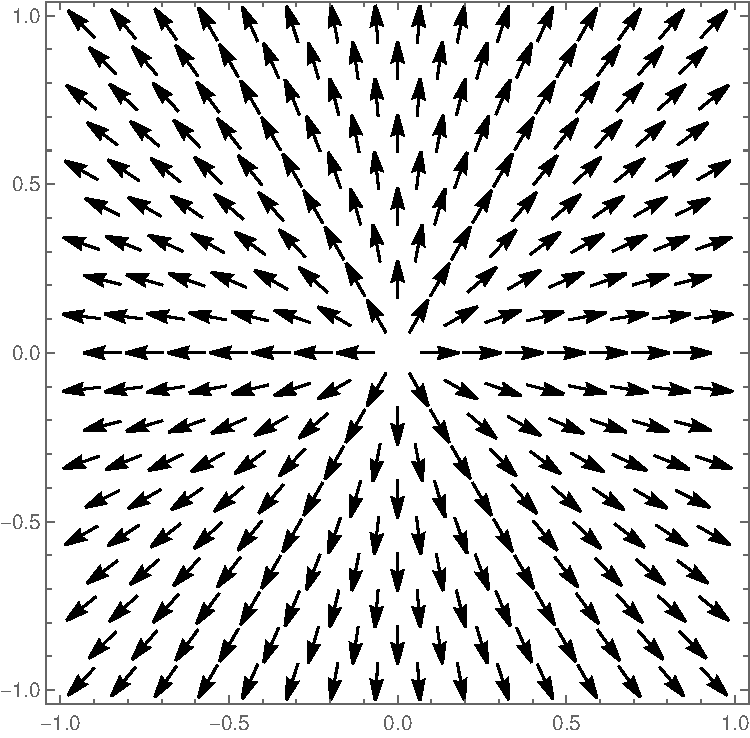
\includegraphics[scale=1,trim= 120 100 100 100,clip]{./figures/vortex.pdf}
		\caption{$n=1$}
	\end{subfigure}
	\begin{subfigure}{0.45\textwidth}
		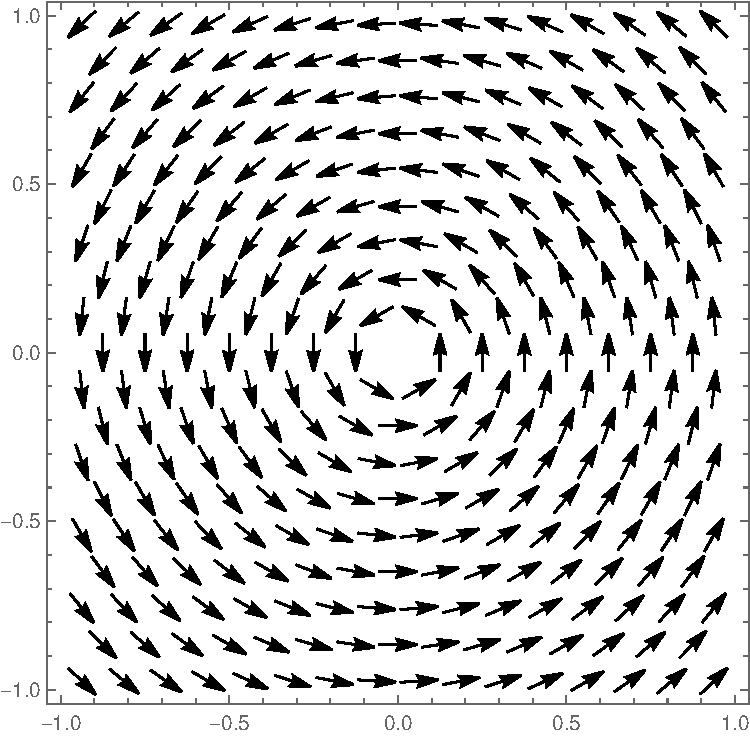
\includegraphics[scale=1,trim= 120 100 100 100,clip]{./figures/vortex2.pdf}
		\caption{$n=1$}
	\end{subfigure}
	
	\begin{subfigure}{0.45\textwidth}
		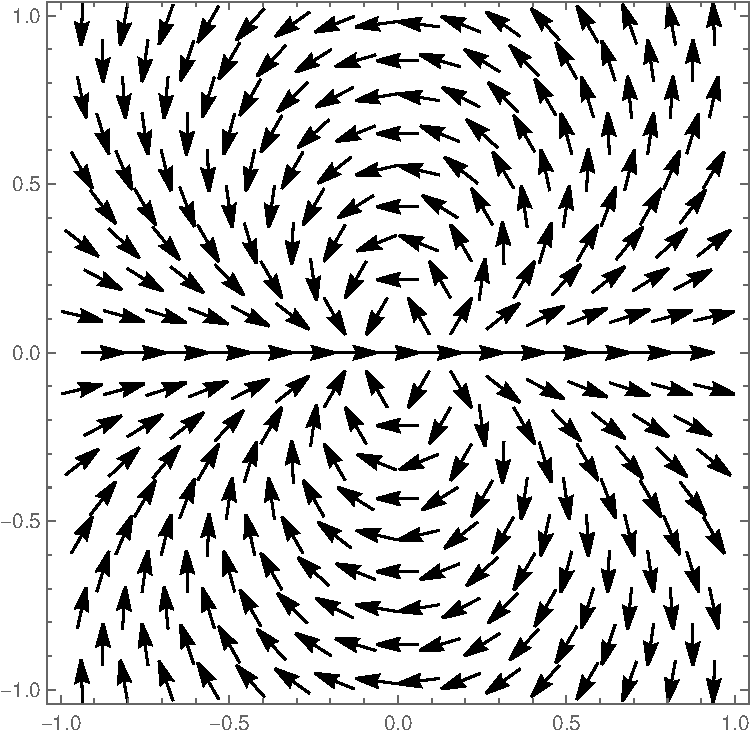
\includegraphics[scale=1,trim= 120 100 100 100,clip]{./figures/vortexn=2.pdf}
		\caption{$n=2$}
	\end{subfigure}
	\begin{subfigure}{0.45\textwidth}
		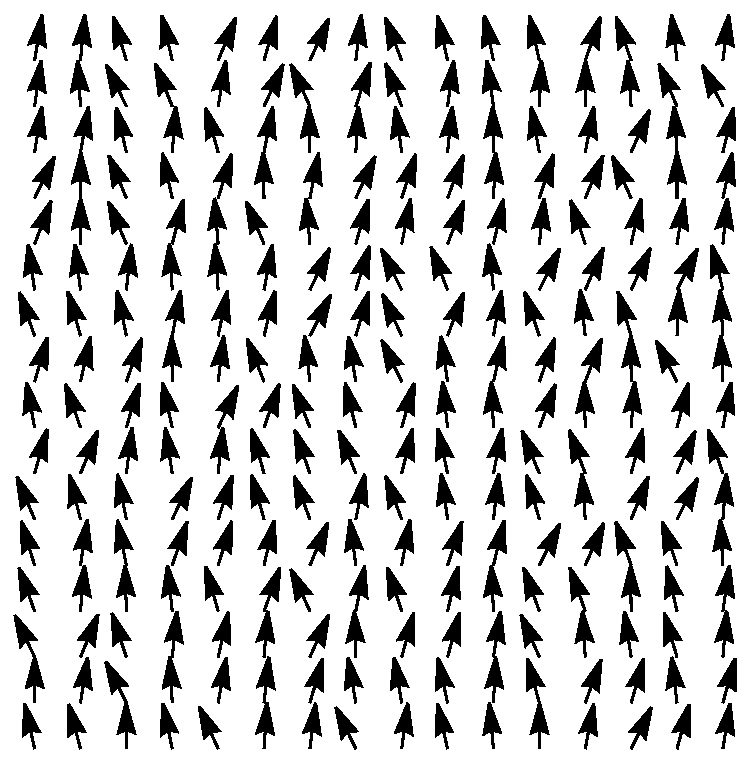
\includegraphics[scale=1,trim= 120 100 100 100,clip]{./figures/n0conf2.pdf}
		\caption{$n=0$}
	\end{subfigure}
	\begin{subfigure}{0.45\textwidth}
		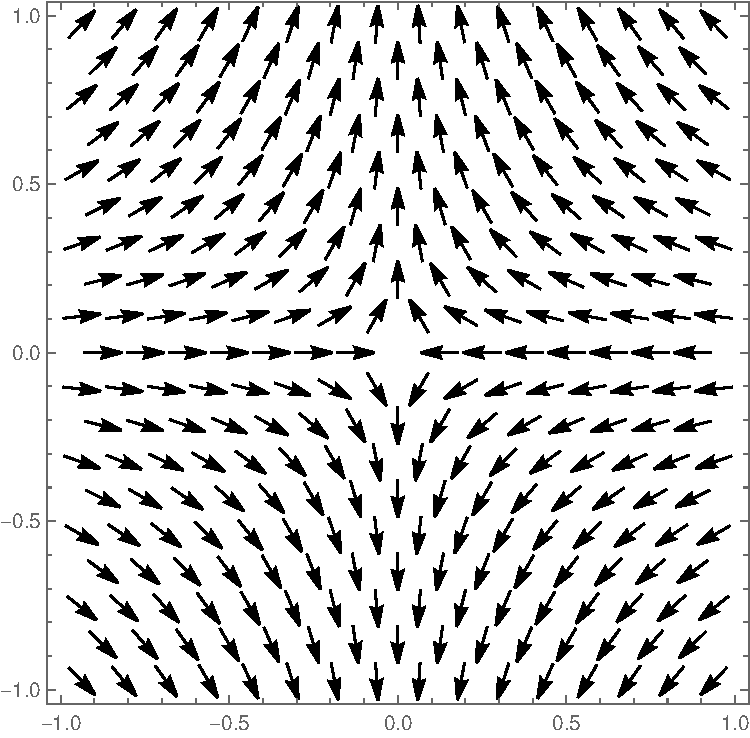
\includegraphics[scale=1,trim= 120 100 100 100,clip]{./figures/n=-1.pdf}
		\caption{$n=-1$}
	\end{subfigure}
	\begin{subfigure}{0.45\textwidth}
		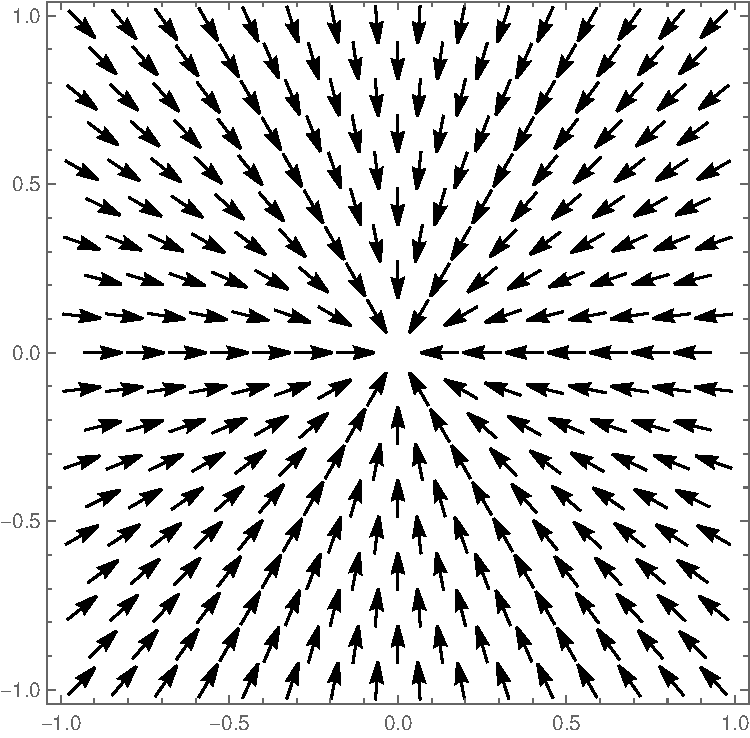
\includegraphics[scale=1,trim= 120 100 100 100,clip]{./figures/n=-1s.pdf}
		\caption{$n=1$}
	\end{subfigure}
	\caption{Configurations of spins with different winding numbers.}
	\label{fig:vortices}
\end{figure}
When we stack vortices on top of each other we can create a 1-dimensional defect called a \textit{string}, see Figure \ref{fig:string}.

\begin{figure}
	\centering
	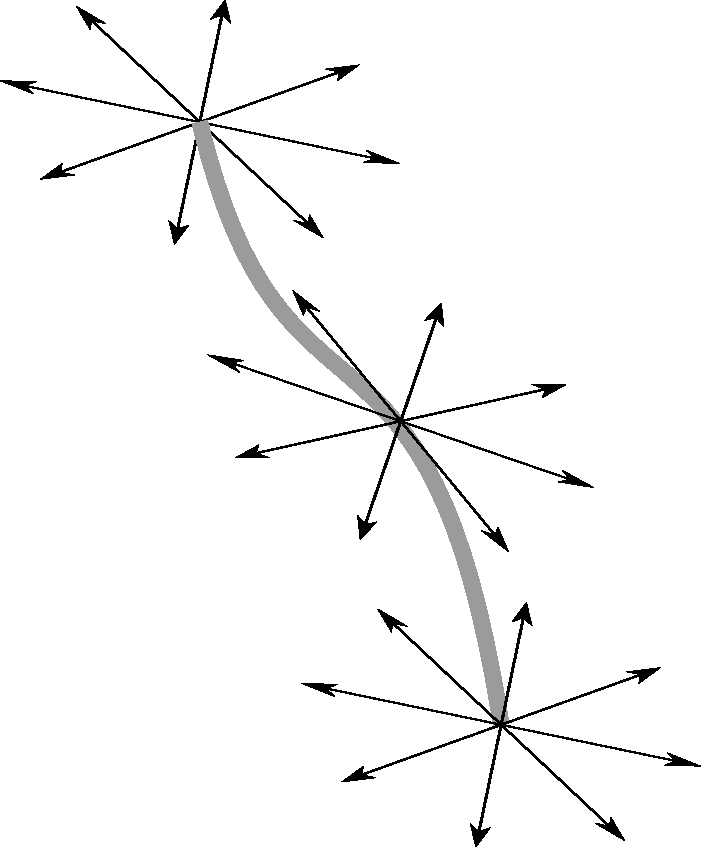
\includegraphics[scale=0.7]{./figures/string.pdf}
	\caption{Two dimensional vortices stack on top of each other in the 3-dimensional physical space forming a vortex \textit{string}.}
	\label{fig:string}
\end{figure}
%\subsection{Flux lines in type II superconductors}
\subsection{Nematics}\label{sec:nematics}
Liquid crystals are substances that share properties from both liquids and crystals. Liquid crystals possess phases such as the nematic phase, the chollesteric phase, smectic phase, etc. Nematics are liquid crystals in the nematic phase. Nematics are made of rod shaped molecules which tend to align parallel to one another. Since the orientation of the molecules does not matter, mathematically the order parameter is represented by a headless vector, $\vec{n} \equiv -\vec{n}$.


In this case, the group of symmetries of the physical 3d space is $G=\text{SO}(3)$. The group of isometries $H=D_{\infty}$ are rotations along the molecular axis and the rotations along the axis perpendicular to the molecular axis. Then, the order parameter space is $G/H = \text{SO}(3)/D_{\infty}$, which is known to be isomorphic to the real projective plane $RP^2$. The real projective plane $RP^2$ is the space formed by all lines that pass the origin in $\mathbb{R}^3$, and it is described as a half-sphere with opposite points in the equator identified. Through a direct application of the Seifert-van Kampen theorem, it can be shown that $\pi_1(RP^2) \simeq \mathbb{Z}_2$. A heuristic explanation of this fact can be described as follows: the space $RP^2$ is an hemisphere and can be flatten out to become a flat disk with the build only two types of loops, one type that is entirely inside the disk, and another one connecting two opposite points in the boundary, see Fig.\ \ref{fig:rp2}. The one inside the disk is a trivial loop since it can be reduce to a point, because $RP^2$ is simply connected within the disk. However, the one that connects opposite points in the boundary cannot be reduce to a point since the points in the boundary are fixed and cannot move. Only this class of non-trivial loop exists, so we conclude that $\pi_1(RP^2)\simeq \mathbb{Z}_2$. In conclusion, nematics enable one type of vortices. 

\begin{figure}
\centering
	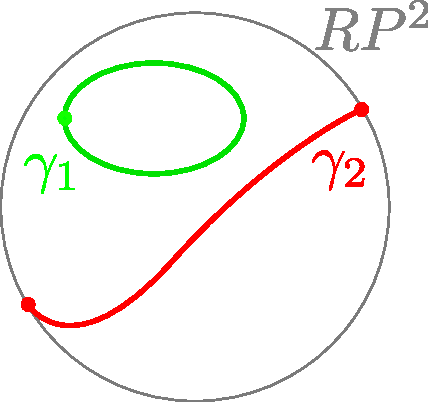
\includegraphics[scale=0.7]{./figures/rp2.pdf}
	\caption{The projective plane $RP^2$ and two types of loops $\gamma_1$ and $\gamma_2$. The loop $\gamma_1$ is a trivial loop and can be contracted to a point. However, $\gamma_2$ is a loop that connects two opposite points on the boundary, and it is the only type of loops which cannot be contracted to a point.}
	\label{fig:rp2}
\end{figure}

\begin{figure}
\centering
	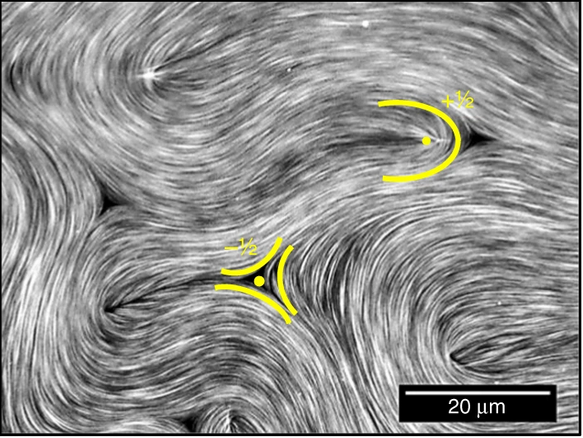
\includegraphics[scale=0.5]{./figures/vortexnematics.png}
	\caption{Vortices in a nematic represented as yellow dots with topological charges 1/2 and $-1/2$, figure taken from Ref.\ \cite{Doos2018}.}
	\label{fig:vortexnematic}
\end{figure}

However, if we constrain the molecules to live in a plane, the order parameter manifold is now a semicircle with the endpoints identified, denoted as $S^1/\mathbb{Z}_2$. The semicircle is mathematically described by $x=e^{i\varphi}$, $\varphi\in [0,\pi)$ and can be mapped to a complete circle by the function $f(x) = x^2$. Thus, the space $S^1/\mathbb{Z}_2$ is isomorphic to $S^1$. Therefore, its  first homotopy group is $\pi_1(S^1/\mathbb{Z}_2 \simeq S^1) \simeq \mathbb{Z}$. In some applications, it is convenient to take $\pi_1(S^1) \simeq \frac{1}{2}\mathbb{Z}$, since $\mathbb{Z}\simeq \frac{1}{2}\mathbb{Z}$, so the topological charge can be an integer or half-integer. In Figure \ref{fig:vortexnematic}, we see two types of vortices in a nematic with topological charges of $1/2$ and $-1/2$.

\subsection{Quantum vortices in superfluid helium}\label{sec:helium}
Helium has two isotopes, $^3$He and $^4$He, and when they become superfluids, they exhibit rotating vortex defects when stirred.

In the case of $^4$He, it becomes a superfluid only when it is cooled down below 2.17 K, and since it is a boson, its superfluid phase is related to the Bose-Einstein condensation. 

In contrast, $^3$He, the lighter helium isotope, only becomes a superfluid when its temperature drops below 0.0025 K. Since $^3$He is a fermion, its superfluid phase has a different mechanism from $^4$He. $^3$He superfluid is related to the creation of Cooper pairs (similar to superconductivity). $^3$He has two superconductivity phases and when an external magnetic field is applied to one of the phases it splits creating yet another superconducting phase.

The order parameters for $^3$He and $^4$He are their multi-particle wave functions, a complex scalar for $^4$He and a $3\times 3$ complex matrix for $^3$He. In $^4$He, we can define a Lagrangian which is symmetric under $\text{U}(1)$ that is related to global phase transformations of the wave function. However, this $\text{U}(1)$ can break since in a state like a superfluid there exists a non zero superfluid condensate. This condensate has a definite phase, so it breaks the $\text{U}(1)$ symmetry down to $I$. %its wave function satisfies the Schrödinger equation, and it is known to possess a U$(1)$ symmetry, 
 So $\pi_1(\text{U}(1)/I\simeq S^1) \simeq \mathbb{Z}$, therefore $^4$He has vortices. In fact, these vortices have their circulation quantized, so they are called quantum vortices. In order to see this, let us consider a system with $N$ bosonic particles. The wave function of $^4$He superfluid takes the form
\begin{equation}
	\psi = A e^{i\varphi(\vec{r}_1,\vec{r}_2,\dots,\vec{r}_N)},
\end{equation}
where $\varphi = \sum_i \vec{p}_{s,i}\cdot\vec{r}_i/\hbar$ and $\vec{p}_{s,i}= m \vec{v}_{s,i}$, where $m$ and $\vec{v}_{s,i}$ are the mass of  individual $^4$He atoms and the drift velocity, respectively. With this definition of the phase $\varphi$, it is straightforward that
\begin{equation}
	\vec{v}_s = \frac{\hbar}{m}\nabla \varphi.
\end{equation}
Since $\varphi$ is continuous, that means that the integral along a closed path surrounding the vortex core must be an integer multiple of $2\pi$,
\begin{equation}
	\oint d \varphi = 2\pi n, \ n\in\mathbb{Z},
\end{equation}
similar to what we encountered in the planar spin model. Computing the circulation of the vortex results in
\begin{equation}
	\Gamma = \oint \vec{v}_s \cdot d\vec{l} = \frac{nh}{m}.
\end{equation}

Experimentally, quantum vortices appear when the vessel containing $^4$He superfluid is rotated. At low angular velocities, the superfluid remains at rest while the vessel is rotated. At higher velocities, vortices appear and rotate. Ref.\  \cite{PhysRevLett.43.214} reported the first experimental observation of vortices in superfluid $^4$He. In Figure \ref{fig:heliumvortices} we see vortices formed in superfluid $^4$He droplets from numerical simulations, image taken from Ref.\ \cite{ancio2015}.

\begin{figure}
	\centering
	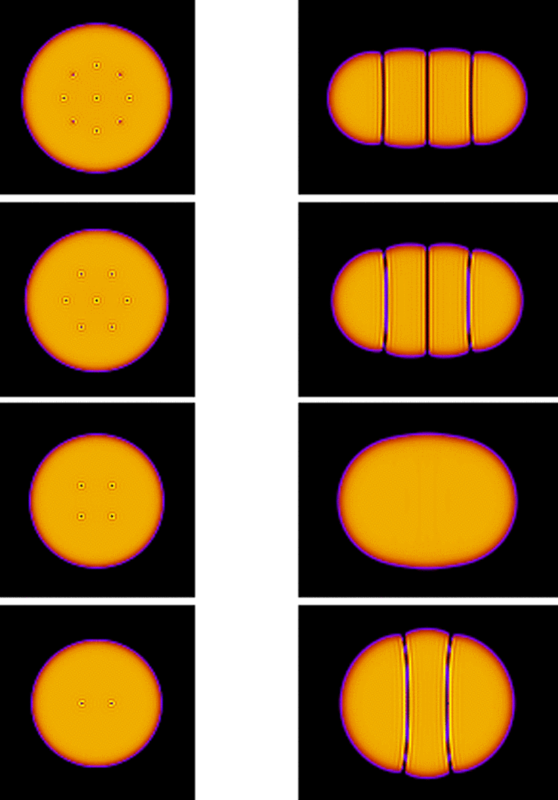
\includegraphics[scale=0.5]{./figures/hevortices.png}
	\caption{Quantum vortices in superfluid $^4$He droplets, generated by numerical simulations. We see from top to bottom, 9, 7, 4 and 2 vortices. Left panel: top view parallel to the angular momentum, $z=0$. Right panel: side view perpendicular to the angular momentum,  $x=0$. Image taken from Ref.\ \cite{ancio2015}} %The container with the superfluid is rotated, and vortices appear when there a certain threshold in the velocity is attained.}
	\label{fig:heliumvortices}
\end{figure} 


\section{Quantum field theory}\label{sec:qft}

\subsection{The vacuum as the order parameter manifold}\label{sec:vacuum}
Let us consider a theory with a scalar field $\phi$, which transforms under a representation of a Lie group of transformations $G$. Let the potential $V = V(\phi)$ be a function of the fields invariant under transformations of $G$.

If the potential  $V$ acquires a non-zero vacuum expectation value (VEV) $\phi_0$, then the symmetry group $G$ will be spontaneously broken, so $\phi$ develops a set $\mathcal{M}$ of degenerate vacua, this implies $\phi_0 \in \mathcal{M}$. All the transformations of $\phi_0$ by representations of $G$ will be genuine VEVs of the scalar field, that is, $D(g)\phi_0 \in \mathcal{M}$. Some of these transformations may lead to the same point. We define the subgroup $H\subset G$ as the group of elements of $G$ which leave $\phi_0$ invariant, that is,
\begin{equation}
	H = \{g\in G | D(g)\phi_0 = \phi_0\}.
\end{equation}
%We wish to determine the set of all possible vacua of the field $\phi$. %This set is given by all non-trivial transformations in $G$ of $\phi_0$. 
This implies that the set of all distinct transformations of $\phi_0$ is given by the quotient group $G/H$, which means that the vacuum manifold is $\mathcal{M}=G/H$.%Let $D(g)$ be a transformation that takes $\phi_0$ to some other point $\phi_1$.
%Then all the elements that take $\phi_0$ to the same point, that is, $D(g)\phi_0 = D(g')\phi_0$ if and only if $D(g') = D(g)D(h) = D(g\cdot h)$ with $h\in H$, 

In other words, the set of values of a scalar field that minimizes the potential, in a theory where a group of symmetries $G$ breaks spontaneously down to a subgroup $H\subset G$, forms a manifold which we identify as the coset space $G/H$. This way, we can take the vacuum manifold as the order parameter manifold, and the order parameter as a state in the vacuum.

%In field theory we sometimes are interested in static solutions to the field equations with a definite energy which we call \textbf{solitons}.
%\begin{definition}
%A \textbf{soliton} as solutions to field equations with the following properties:
%\begin{enumerate}
%\item The energy density is finite and localized in space.
%\item They preserve their shape while propagating at constant speed. From this it follows that they are static in time.
%\end{enumerate}
%\end{definition}



\subsection{Vacuum topology}\label{sec:vactop}

 Let us consider a Lagrangian density of a complex scalar field $\phi(x) = \phi(t,\vec{x})\in \mathbb{C}$ as
\begin{equation}
	\mathcal{L} = \frac{1}{2}\partial^{\mu} \phi^* \partial_{\mu} \phi  - V(\phi).
\end{equation}
Then its energy density is
\begin{equation}
		\epsilon = \frac{1}{2}|\partial_t \phi|^2 + \frac{1}{2}|\nabla \phi|^2 + V(\phi).
\end{equation}
For the total energy of the derivative terms to be finite, we require that
\begin{equation}
	\lim_{|\vec{x}|\to\infty} \phi(x) \in \mathcal{M},
\end{equation}
which means that at spatial infinity the field configuration $\phi$ takes a value in the vacuum manifold $\mathcal{M}$. The value of the field can be different in different directions at spatial infinity. Therefore, a field configuration defines a map from $S^{d-1}_{\infty}$, the $(d-1)$-sphere at the spatial infinity in $\mathbb{R}^d$, to the vacuum manifold $\mathcal{M}$
\begin{equation}
	\phi^{\infty} : S^{d-1}_{\infty}\to\mathcal{M},
\end{equation}
which means that the map $\phi^{\infty}$ defines a $(d-1)$-loop in $\mathcal{M}$.
As we saw earlier, two field configurations $\phi$ and $\phi'$ are homotopic, or topologically equivalent, if their field configurations at infinity $\phi^{\infty}$ and $\phi'^{\infty}$ can be deformed continuously into one another, that is, if they fall into the same equivalence class. This suggests that the topological information of the field configurations is com\-plete\-ly defined by the homotopy group of the vacuum manifold $\pi_{d-1}(\mathcal{M})$.

%It is known that in a linear field theory (linear in the equations of motion), two field configurations are homotopic if they have the same asymptotic behavior. However, two field configurations $\phi$, $\phi'$ can still be homotopic even if their asymptotic values $\phi^{\infty}$ and $\phi'^{\infty}$ are different, as long as these two are homotopic. This implies that the topological information of the field configuration is completely defined by the homotopy class of the map $\phi^{\infty}$ which is an element of $\pi_{d-1}(\mathcal{M})$.

\subsection{The Kibble mechanism}\label{sec:kibble}

 Several phase transitions took place in the early universe due to the cooling down of the universe as a consequence of its expansion. The fast expansion, at the late stages of inflation, produced casually uncorrelated regions because the correlation length $\sim H^{-1}$ was shorter than the size of the universe, where $H$ is Hubble's parameter. These regions, in principle, could have different configurations of vacuum states for some field. At some instant, the correlation length grew faster than the expansion rate of the universe, so the regions grew and became casually connected. In the interfaces between these regions, topological defects could form. The mechanism of having topological defects due to phase transitions in the early universe is known as the \textit{Kibble mechanism} \cite{Kibble1976,Kibble1980}. 
 
 %An example of the Kibble mechanism is the one that produces \textit{cosmic strings}. 


\section{The Standard Model}\label{sec:SM}
In the Standard Model of particle physics, particles are classified as either fermions or bosons, where fermions are particles with half-integer spin and bosons with an integer spin. 

A refined classification of fermions distinguishes between leptons and quarks, where only the quarks posses color charge. Also, fermions in general have left- or right-handed chirality. For massless fermions they are in\-de\-pend\-ent of each other. 

 Leptons possess a quantum number called the \textit{lepton number} $L$. Each particle in the lepton family is assigned a lepton number of $L=1$. Similarly, quarks posses a \textit{baryon number} $B$, and each quark is given a baryon number of $B=1/3$. Moreover, we assign $L=-1$ and $B=-1/3$ to the anti-leptons and anti-quarks, respectively. In nature, only combinations of quarks that give an integer baryon number are realized; they are called hadrons. 

Bosons with a spin 1 in the Standard Model are called the force carriers, such as the photon that is the electromagnetic force carrier, the gluons that mediate the strong interaction and the $W^{\pm}$, $Z$ bosons which mediate the weak interaction. Finally, the Higgs boson is the only elementary scalar particle, with spin 0. Along with Yukawa couplings, it is responsible of giving mass to other elementary particles.

There are two kinds of symmetries in physics: global symmetries and local or gauge symmetries. Normally, global symmetries are approximate, they arise from a hierarchy of energy scales and are manifest in the form of multiplets of particles. For example, in QCD with massless quarks the only dimensionful quantity is $\Lambda_{\text{QCD}}\sim 300$ MeV and since the masses of the up and down quarks are far below this energy scale, there is an approximative SU$(2)$ symmetry known as the isospin  symmetry. On the other hand, gauge symmetries are redundancies in the formulation and are impossible to break. However, there is no fundamental reason for a global symmetry not to break. There are exceptions to the rule, one of them is Lorentz global symmetry that is related to CPT invariance. 
In the Standard Model of  particle physics, there is another exact global symmetry: the difference between the baryon and lepton number is conserved. 

\subsection{The global U$(1)_{B-L}$ symmetry}\label{sec:globalU} 
It is known that by Noether's theorem, both lepton and baryon vector currents are conserved classically. For leptons and quarks, their corresponding currents read
%(with Dirac neutrinos)
\begin{eqnarray}
	j_L^{\mu} & = & \sum_{f\in\text{lepton}} \left[\bar{f}_L \gamma^{\mu}f_L+\bar{f}_R \gamma^{\mu}f_R \right]\nonumber\\
	j_B^{\mu} & = & \sum_{q\in\text{quarks}} \left[\bar{q}_L \gamma^{\mu}q_L+\bar{q}_R \gamma^{\mu}q_R \right].
\end{eqnarray}
As we mentioned, at the classical level these currents are conserved,
\begin{eqnarray}
	\partial^{\mu}j_{\mu}^L & = & 0\nonumber\\
	\partial^{\mu}j_{\mu}^B & = & 0,
\end{eqnarray}
which implies both lepton and baryon number conservation. Upon quantiza\-tion, we do not expect any anomalies in these vector currents. We only expect an anomaly in the axial current,
\begin{equation}
	j^{\mu}_5  =  \sum_{f\in\text{lepton}} \left[\bar{f}_L \gamma^5\gamma^{\mu}f_L+\bar{f}_R \gamma^5\gamma^{\mu}f_R \right].
\end{equation}
However, this is not the complete picture, in fact, the anomaly can be moved from the axial current to the vector current through a gauge invariant regularization, as reviewed in Ref.\ \cite{10.1088/978-1-6817-4457-5}. 

In fact, upon quantization the same divergence in the vector currents in both leptonic and baryonic sector arise
\begin{eqnarray}
	\partial^{\mu}j_{\mu}^L & = &-\frac{N_g g^2}{32\pi^2}\text{Tr}[W_{\mu\nu}\tilde W^{\mu\nu}]\nonumber\\
		\partial^{\mu}j_{\mu}^{B} & = & -\frac{N_g g^2}{32\pi^2}\text{Tr}[W_{\mu\nu}\tilde W^{\mu\nu}],
\end{eqnarray}
where $W^{\mu\nu}$ is the $\text{SU}(2)_L$ field strength tensor in the Standard Model, $\tilde W^{\mu\nu} = \epsilon_{\mu\nu\rho\sigma}W^{\rho\sigma}$, $g$ is the weak gauge coupling and $N_g$ is the number of fermion generations.

Theoretically, these anomalous currents allow for the baryon or lepton number violation; however, no process that realizes such violation has ever been observed experimentally. If violations of the baryon number exist, there are several ways that a proton can decay while preserving the laws of energy conservation, angular momentum conservation, and electric charge con\-ser\-va\-tion. We list some examples of proton channel decays \cite{Primakoff1981}
\begin{gather} 
 p \to e^+ \bar{\nu}_e{\nu}_e, \ \ \ p \to  e^+e^+  e^- ,\ \ \ p \to  e^+\mu^+  \mu^-,\nonumber \\
 p \to e^+ \gamma,\ \ \ p \to \mu^+\gamma, \nonumber\\
 p  \to  e^+ \pi^0,\ \ \ p  \to  \bar{\nu}_e\pi^+, \ \ \ p  \to  \mu^+ K^0, \ \ \ p  \to  \bar{\nu}_{\mu}K^+.
\end{gather}
In all these processes, the charge $B-L=1$ is conserved, where $B\in\{1,0\}$ and $L\in\{0,-1\}$. In order to explain the conservation of the $B-L$ charge theoretically, we define a new current $j_{\mu}^{B-L}=j_{\mu}^B-j_{\mu}^L$, which satisfies
\begin{equation}
	\partial^{\mu}(j_{\mu}^{B-L}) = 0.
\end{equation}
This implies the conservation of the $B-L$ charge.
Conservation of the $B-L$ charge is associated with a global U$(1)$ symmetry, which we call U$(1)_{B-L}$.% We wonder if possibly a particle could mediate processes that conserve $B-L$ charge. 

\chapter{Cosmic strings}\label{chap:cosmic}
The understanding of spontaneous symmetry breaking and cosmological phase transitions has led us to think about the possible existence of topological defects formed in the early universe. Topological defects are related to spontaneous symmetry breaking since they give rise to a non-trivial vacuum manifold. For instance, the spontaneous symmetry breaking of a global or local U(1) symmetry can lead to 1-dimensional topological excitations known as vortices, and when these vortices form lines in the 3-dimensional space they are called vortex strings. 
 
\section{The creation of cosmic strings in the early universe} 
Let us illustrate the formation of cosmic strings through the Kibble mech\-an\-ism. Suppose we have a field theory, with a complex order parameter scalar field $\phi$, with a $\text{U}(1)$ symmetry and with a potential suitable for spontaneous symmetry breaking to happen. Due to high temperatures in the early universe, the field con\-fig\-u\-ra\-tions initially remained in a state of unbroken symmetry. When the temperature decreased as the universe expanded, spontaneous symmetry breaking occurred and different regions of the universe remained isolated from each other. In each isolated region, the field acquired a different vacuum expectation value. The patches grew and became casually connected giving rise to topological defects. If these uncorrelated regions formed a loop around some line such that the field values along the loop completed $n$ turns, the topological defect is in fact a \textit{cosmic string} with a winding number of $n$, see Figure \ref{fig:higgspotential}. %and if the  In this example, since we are dealing with a U(1) symmetry in a 3-dimensional space, the topological defects are in fact strings which we call \textit{cosmic strings}.
\begin{figure}
	\centering
	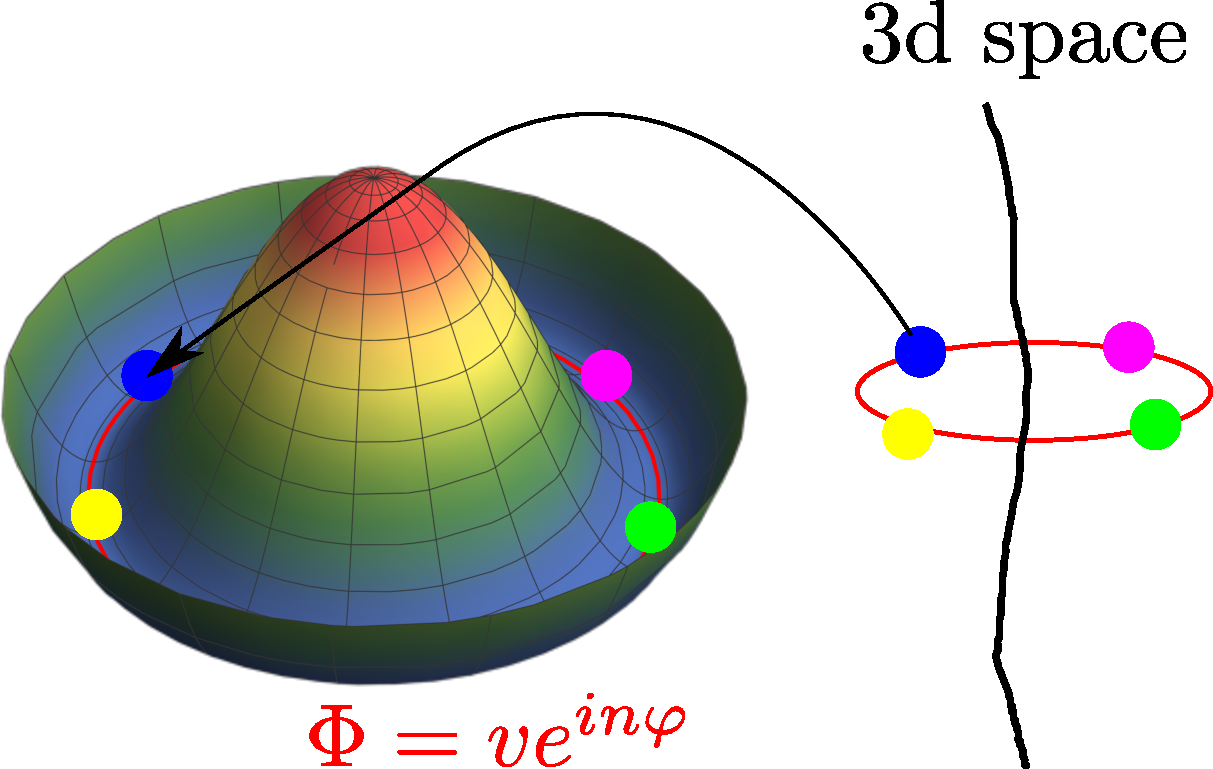
\includegraphics[scale=0.65]{./figures/higgspot.pdf}
	\caption{The formation of a cosmic string. When different uncorrelated points in the universe became casually connected, the different vacuum-values the field took in these points gave rise to topological defects.}
	\label{fig:higgspotential}
\end{figure} 
%\begin{figure}
%	\centering
%	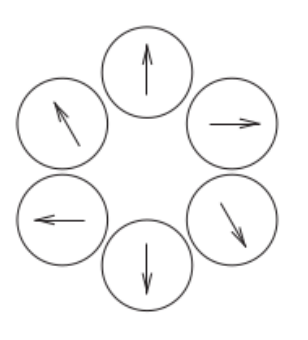
\includegraphics[scale=0.5]{./figures/vortex.png}
%	\caption{Vortex.}
%	\label{fig:vortex}
%\end{figure} 
\section{Global cosmic strings}\label{sec:global}
We consider the simplest model where string-like solutions appear: a scalar field $\phi(x)\in\mathbb{C}$ with a global U(1) symmetry and a Lagrangian density given by
\begin{equation}
	\mathcal{L} = \frac{1}{2}\partial^{\mu} \phi^* \partial_{\mu} \phi  \underbrace{-\frac{m^2}{2} |\phi|^2 - \frac{\lambda}{4}|\phi|^4-\frac{\lambda}{4}v^4}_{-V(\phi)} ,
\end{equation}
where $m^2$ and $\lambda$ refer to the renormalized values.
We require $\lambda>0$, in order for the potential to be bounded from below. We find the potential minima by differentiating with respect to $|\phi|$
\begin{equation}
	\left.\frac{dV}{d|\phi|}\right|_{\phi_0\in\mathcal{M}} = m^2 |\phi_0|+\lambda |\phi_0|^3 = 0 \Rightarrow \begin{cases} |\phi_0|^2 = -\frac{m^2}{\lambda} \text{ only if } m^2<0 \\ 
	|\phi_0| = 0 \text{ if } m^2 \geq 0.
	\end{cases}
\end{equation}
If $m^2 < 0$, it leads to the spontaneous symmetry breaking of the U(1) symmetry. Then the vacuum expectation value is
\begin{equation}
	|\phi_0| = v \equiv \sqrt{\frac{-m^2}{\lambda}}.
\end{equation}
We consider a cylindrically symmetric, static field configuration
\begin{equation}
	\phi = \phi(r,\varphi,z) = \phi (r,\varphi) .
\end{equation}
At $r \to \infty$, the field configuration $\phi$ must take its vacuum expectation value $v$, $\lim\limits_{r\to\infty}|\phi(r,\varphi)| = v$. But the complex phase can be any differentiable function of $\varphi$. Therefore our ansatz takes the form
\begin{equation}
	\lim_{r\to\infty}\phi(r,\varphi) = \phi^{\infty}(\varphi) = v e^{i\chi(\varphi)} . 
\end{equation}
The function $\phi^{\infty}$ maps $S^1 \to \mathcal{M} = S^1= $ U$(1)$. Since $\pi_1[S^1] = \mathbb{Z}$, the model allows for vortex solutions and there is a winding number $n\in\mathbb{Z}$. Global strings are configurations with $n\neq 0$, which are topologically stable, i.e., stable under continuous deformations. We assume $\chi(\varphi) = n\varphi$ with $n\neq 0$. Our ansatz becomes
\begin{equation}
	\phi(r,\varphi) = f(r)e^{in\varphi},
\end{equation}
where 
\begin{equation}
	\lim_{r\to\infty}f(r) = v,\ \ \ f(0) = 0.
	\label{eq:limits} 
\end{equation}
The latter relation is due to the fact that the field $\phi$ must be single valued. The field equation of motion reads
\begin{equation}
	\partial^{\mu}\partial_{\mu}\phi = -m^2\phi -\lambda |\phi|^2 \phi ,
\end{equation}
using cylindrical coordinates
\begin{eqnarray}
	\frac{1}{r} \partial_{r} (r\partial_{r}\phi) + \frac{n^2}{r^2}\partial_{\varphi} \phi = m^2 \phi + \lambda |\phi|^2 \phi \nonumber \\
	\frac{1}{r} \partial_{r} (r f')e^{i\varphi} - \frac{n^2}{r^2} f e^{i\varphi} = m^2 fe^{i\varphi} + \lambda f^3 e^{i\varphi} \nonumber \\
	\label{eq:global_str}
	f'' + \frac{1}{r}f'- \frac{n^2}{r^2} f = m^2 f+ \lambda f^3.
\end{eqnarray}
We arrive at a non-linear second order differential equation. We can obtain its asymptotic behavior at large $r$ and near zero, with the constraints of eq. \eqref{eq:limits}.
If $r\approx 0$, we only keep the linear powers of $f$, so eq. \eqref{eq:global_str} simplifies to
\begin{equation}
	f'' + \frac{1}{r}f'- \frac{n^2}{r^2} f -m^2 f\approx  0.
\end{equation}
Inserting $m^2 = -v^2\lambda$, we obtain
\begin{equation}
	f'' + \frac{1}{r}f'- \frac{n^2}{r^2} f + v^2\lambda f\approx  0.
\end{equation}
If we substitute $u=\sqrt{v^2\lambda}r$, then $f(r) = \tilde{f}(u)$ and we obtain Bessel's equation for $\tilde f$
\begin{equation}
	\frac{d^2\tilde f}{du^2} + \frac{1}{u}\frac{d\tilde f}{du}+\left(1- \frac{n^2}{u^2}\right) \tilde f\approx  0\, ,
\end{equation}
with the solution
\begin{equation}
	\tilde f(u) \approx  f_0 J_{|n|}(u) +  \tilde f_1 Y_{|n|}(u),
\end{equation}
where $J_{|n|}$ and $Y_{|n|}$ are the Bessel functions of the first and second kind of order $n$, respectively, and $f_0$ and $\tilde f_1$ are real constants. We set $\tilde f_1=0$ since $Y_{|n|}$ diverges at zero.
Then the solution is
\begin{equation}
	\tilde f(u) \approx f_0 J_{|n|}(u) = f_0 J_{|n|}(\sqrt{v^2\lambda}r)\, .
\end{equation}
Therefore
\begin{equation}
	f(r) \approx f_0 J_{|n|}(\sqrt{v^2 \lambda}r) = f_0\sum_{m=0}^{\infty}\frac{(-1)^m}{m!\Gamma(m+|n|+1)}\left(\frac{\sqrt{v^2 \lambda}r}{2}\right)^{2m+|n|}
\end{equation}
and to order $n$ in $r$ we have
\begin{equation}
	f(r) \approx f_0 \frac{1}{|n|!}\left(\frac{\sqrt{v^2 \lambda}r}{2}\right)^{|n|}.
	\label{eq:solr0}
\end{equation}
%The absolute value of $|n|$ comes from the fact that when $n\to-n<0$, $J_{-n}=(-1)^nJ_n$.
%Making the ansatz $f(r) = f_0 r^l$ we arrive to $l = \pm n$. So
%\begin{equation}
%	f(r) \approx f_0 r^n + \tilde f_0 r^{-n}
%\end{equation}
%where $f_0$ and $\tilde f_0$ are real constants. Since $f(0)=0$, we need a solution that does not explode at $r = 0$. If $n>0$ we take $f_0 r^n$ and if $n<0$ we take $\tilde f_0 r^{-n}$. Combining these two results we get
%\begin{equation}
%	\label{eq:phi_r0}
%	f(r) \approx f_0 r^{|n|} \text{ when } r\approx 0 \, .
%\end{equation}
At $r\to\infty$, $f(r)$ approaches its vacuum expectation value $v$. If we write in this limit $f(r) = v + \delta f(r)$, and ignoring O$(\delta f^2)$ terms, eq.\ \eqref{eq:global_str} turns into an equation for $\delta f$
\begin{equation}
	 \delta f'' +\frac{1}{r}\delta f'- \frac{|n|^2}{r^2}\delta f -2v^2\lambda\delta f \approx 0\, .
\end{equation}
When we perform the change of  variable $u=\sqrt{2\lambda}vr$ the equation above turns into the modified Bessel equation
\begin{equation}
\frac{d^2 }{du^2}\delta f + \frac{1}{u} \frac{d}{du}\delta f - \left(1+\frac{|n|^2}{u^2} \right)\delta f \approx 0\,.
\end{equation}
This equation has the solution
\begin{equation}
	\delta f \approx \tilde f_0I_{|n|}(u) + f_1 K_{|n|}(u) = \tilde f_0 I_{|n|}(\sqrt{2\lambda}vr) + f_1 K_{|n|}(\sqrt{2\lambda}vr)
\end{equation}
where $I_{|n|}$ and $K_{|n|}$ are the modified Bessel function of the first and second kind, respectively, and $\tilde f_0$ and $f_1$ are real constants. Since $I_{|n|}$ diverges when $r\to \infty$, we set $\tilde f_0=0$. Hence, the solution for $f$ at $r\to\infty$ takes the form
\begin{equation}
	f(r) \approx v+f_1 K_{|n|}(\sqrt{2\lambda}vr)\, .
\end{equation}

%If we write in this limit $f = v - \delta f$ we get
%\begin{equation}
%	-\frac{n^2}{r^2} \approx m^2 + \lambda (v-\delta f)^2 = m^2 + \lambda v^2 -2\lambda v \delta f + O(\delta f^2).
%\end{equation}
%Thus
%\begin{equation}
%	\delta f \approx \frac{n^2}{2\lambda v r^2}.
%\end{equation}
In summary
\begin{equation}
	\label{eq:asymptotic_global}
	f(r) \approx \begin{cases}
		\displaystyle f_0 \frac{1}{n!}\left(\frac{\sqrt{\lambda}vr}{2}\right)^{|n|}& r \ll 1 \\
	\displaystyle v+f_1\sqrt{\frac{\pi}{2\sqrt{2\lambda}v}}r^{-1/2}e^{-\sqrt{2\lambda}vr} & r \gg 1\, ,
				\end{cases}
\end{equation}
where in the second line we used the asymptotic behavior of $K_n$. %If we consider $n<0$, we find similar behaviors of the solution at the limits. we may write the winding number in the solutions as an absolute value $n$. 
\subsection{Energy density}
The expression for the energy density reads
\begin{equation}
	\label{eq:energy_density}
	\varepsilon(r) = \cancelto{0}{\frac{1}{2}|\partial_t \phi|^2} +\frac{1}{2}|\partial_r \phi|^2 + \frac{1}{2}\left|\frac{1}{r}\partial_{\varphi} \phi \right|^2 +\frac{1}{2}|\partial_z \phi|^2   + V(\phi).
\end{equation}
The first term is zero since $\phi$ is a static configuration.
Because of the angular derivative term, the energy density is of O$(1/r^2)$ at large $r$. Thus the energy per unit length along the $z$ direction, inside a cylinder of external radius $R\to \infty$ and internal radius $\delta\to 0$, diverges logarithmically, that is
\begin{equation}
	\frac{E}{z} \sim \int_{0}^{2\pi}d\varphi \int_{\delta}^{R}  dr  \ r\frac{1}{r^2} \propto \lim_{R\to\infty, \delta\to 0}\log \frac{R}{\delta} .
\end{equation}
%We can interpret this divergence due to the interaction of the string with the Nambu-Goldstone Boson given by the imaginary part of the field.
%The main implication of this result is that global strings have infinite length. Otherwise, there will be an infinite energy gap. 
Figure \ref{fig:global_str} shows the profile of a global string type solution of eq.\ \eqref{eq:global_str}, obtained with numerical methods, which is in agreement with the asymptotic behavior specified in eq.\ \eqref{eq:asymptotic_global}. 

\begin{figure}
	\centering
		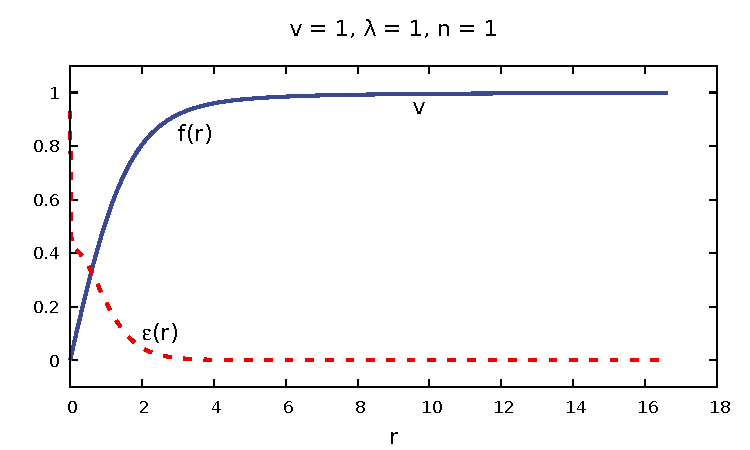
\includegraphics[scale=1]{./figures/global_str.pdf}
	\caption{Radial profile of a global string and its energy density.}
	\label{fig:global_str}
\end{figure}

\section{Local cosmic strings}\label{sec:local}
In order to promote U(1) to a local symmetry, we need to add a gauge field $A_{\mu}$. So the Lagrangian becomes
\begin{equation}
	\mathcal{L} = \frac{1}{2}(D^{\mu} \phi)^* D_{\mu} \phi - \frac{m^2}{2} |\phi|^2 - \frac{\lambda}{4}|\phi|^4 - \frac{\lambda}{4}v^4 - \frac{1}{4}F^{\mu\nu}F_{\mu\nu},
\end{equation}
where $D_{\mu}\phi = (\partial_{\mu} + ihA_{\mu})\phi$ is the covariant derivative, $h$ is a gauge coupling and $F_{\mu\nu} = \partial_{\mu}A_{\nu} - \partial_{\nu}A_{\mu}$ is the field strength tensor. Now, the equations of motion are
\begin{eqnarray}
	D^{\mu}D_{\mu} \phi & = & -m^2 \phi - \lambda|\phi|^2\phi, \\
	D^{\mu}F_{\mu\nu} & = & -\frac{ih}{2}\left[(D_\nu \phi)^* \phi - \phi^* D_{\nu}\phi\right].
\end{eqnarray}
We write the generic, static, cylindrical ansatz as
\begin{equation}
	\phi(r,\varphi) = f(r)e^{in\varphi}, \ \ \ \vec{A}(r,\varphi) = \frac{a(r)}{r}\hat{\varphi},
\end{equation}
where we have chosen the radial gauge where $A_r = 0$. For the functions to be continuous at the origin $f(0) = 0$ and $a(0)=0$.
Using the ansatzë for the functions the equations for $f$ and $a$ take the form
\begin{eqnarray}
	 \label{eq:local_f}
	f'' + \frac{1}{r} f' - \frac{1}{r^2}\left(n+ha\right)^2f- m^2 f- \lambda f^3= 0, \\
	\label{eq:local_a}
	a'' -\frac{1}{r}a'-h(n+ha)f^2= 0.
\end{eqnarray}
From eq.\ \eqref{eq:local_a} we obtain the asymptotic behavior of the function $a(r)$. At large $r$ we expect the function to be constant, this is only achieved if the term in parenthesis is zero, which implies $\lim_{r\to\infty}a(r) = -n/h$.

Again, the system is not analytically solvable, but we can derive its asymptotic behavior.

When $r \to 0$, eq.\ \eqref{eq:local_f} is approximately (assuming $f(r) = $ O$(r)$)
\begin{equation}
	 f'' + \frac{1}{r} f'  -\frac{n^2}{r^2}f -m^2 f\approx 0, 
\end{equation}
so again as in eq.\ \eqref{eq:solr0} the approximate solution is 
\begin{equation}
	f(r) \approx f_0 \frac{1}{|n|!}\left(\frac{\sqrt{v^2 \lambda}r}{2}\right)^{|n|} .
\end{equation}
In this limit, eq.\ \eqref{eq:local_a} takes the form
\begin{equation}
	a'' - \frac{1}{r}a' \approx 0
\end{equation}
and its solution is
\begin{equation}
	a(r) \approx \frac{a_0}{2}r^2,
\end{equation}
where $a_0$ is a constant.

In order to study the limit $r\to\infty$, we use $f = v + \delta f$ and $a = -\frac{n}{h} + \delta a$, and ignore quadratic terms in $\delta f$ and $\delta a$. Then eq.\ \eqref{eq:local_f} takes the form
\begin{equation}
	\delta f''(r) +\frac{1}{r}\delta f'(r)-2v^2\lambda\delta f(r) \approx 0\, .
\end{equation}
with the solution 
\begin{equation}
	\delta f(r) \approx f_1 K_0(\sqrt{2\lambda}v r).
\end{equation}
Considering the limit of large $r$ the function $f$ is approximately
\begin{equation}
	f (r)\approx v + f_1\sqrt{\frac{\pi}{2\sqrt{2\lambda}v}} r^{-1/2}\exp \left(-\sqrt{2\lambda}v r\right),
\end{equation}
where $f_1$ is a real constant, and we used the asymptotic behavior of $K_0$.

Analogously, for eq.\ \eqref{eq:local_a} we may write $a(r) = -\frac{n}{h} - \delta a(r)$. Then we obtain an equation for $\delta a$,
\begin{equation}
	\delta a'' - \frac{1}{r}\delta a' - h^2v^2 \delta a \approx 0,
\end{equation}
and its solution is 
\begin{equation}
	\delta a = a_1 hvr K_1(hv r).
\end{equation}
In this limit of large $r$, the function $a$ behaves as
\begin{equation}
	a \approx -\frac{n}{h} - a_1\sqrt{\frac{\pi h v}{2}} r^{1/2} \exp\left(-hv r \right).
\end{equation}
In summary, we have
\begin{equation}
	\label{eq:fapproxsol}
	f(r) \approx \begin{cases}
		\displaystyle f_0 \frac{1}{|n|!}\left(\frac{\sqrt{v^2 \lambda}r}{2}\right)^{|n|}& r \ll 1 \\
	\displaystyle v+f_1\sqrt{\frac{\pi}{2\sqrt{2v^2\lambda}}}r^{-1/2}e^{-\sqrt{2v^2\lambda}r} & r \gg 1\, ,
				\end{cases}
\end{equation}
and
\begin{equation}
\label{eq:a_asymp}
	a(r) \approx \begin{cases}
		\displaystyle \frac{a_0}{2} r^2& r \ll 1 \\
	\displaystyle -\frac{n}{h} - a_1\sqrt{\frac{\pi h v}{2}} r^{1/2} \exp\left(-hv r \right) & r \gg 1\, .
				\end{cases}
\end{equation}
%If we use the Lorentz gauge, that is, $\square \mathcal{A} = 0$, we can show that the asymptotic solutions  in eq.\ \eqref{eq:a_asymp} are indeed gauge invariant. For static field configurations we have $\square \mathcal{A} = -\nabla^2 \mathcal{A}= 0$ and we can use that $\nabla^2 \mathcal{A} = \nabla (\nabla \cdot \mathcal{A}) - \nabla \times \nabla \times \mathcal{A}$. If we insert $\mathcal{A} = \frac{a(r)}{r}\hat{\varphi}$ in the Laplacian we obtain that it is zero, i.e., the solutions are gauge invariant.

In Figure \ref{fig:local_str} we show an example of the radial profiles of the energy density given by
 \begin{equation}
	\label{eq:energy_density}
	\varepsilon(r) = \cancelto{0}{\frac{1}{2}|\partial_t \phi|^2} +\frac{1}{2}|\partial_r \phi|^2 + \frac{1}{2}\left|\frac{1}{r}\partial_{\varphi} \phi+ih\frac{a(r)}{r}\phi \right|^2 +\frac{1}{2}|\partial_z \phi|^2 +\frac{1}{4}F^{\mu\nu}F_{\mu\nu}  + V(\phi).
\end{equation}
The energy, in this case, is not infinite since the angular covariant derivative $|\frac{1}{r}D_{\varphi}\phi|^2$ vanishes faster than in the global string case when $r\to\infty$. 

For Sections \ref{sec:global} and \ref{sec:local} we follow mainly Refs.\ \cite{Hindmarsh1995,Vilenkin1994}.
\begin{figure}
	\centering
	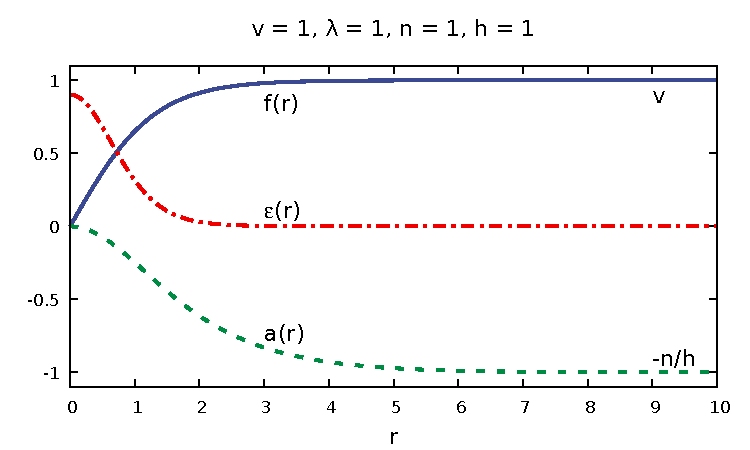
\includegraphics[scale=1]{./figures/local_str.pdf}
	\caption{Local string profile, for the scalar field $\phi$ and $a$ and the energy density $\varepsilon$, as a function of the distance from the core $r$.}
	\label{fig:local_str}
\end{figure}

\section{The mass of a local U$(1)$ string}
By simple arguments, we can estimate the order of magnitude of the mass of a local U$(1)$ cosmic string. The only quantity with dimension is the vacuum expectation value $v$ which has dimension of energy. The tension of the string $\mu$ has dimensions of force, that is, energy squared, therefore
\begin{equation}
	\mu \propto v^2.
\end{equation} 
In order to find the proportionality constant we first perform the following substitution of  $\phi$, $A^{\mu}$ and $x^{\mu}$ to dimensionless variables
\begin{eqnarray*}
	\phi & = & v\tilde \phi \\
	A^{\mu} & = & v\tilde A^{\mu}    \\
	x^{\mu} & = & \frac{1}{hv}\tilde x^{\mu} .
\end{eqnarray*}
This way, the tension of the string reads
\begin{equation}
	\mu = 2\pi v^2 \int_0^{\infty} \tilde rd\tilde r \, \left(\frac{1}{2}\left( D^{\tilde\mu} \tilde\phi\right)^{*} D_{\tilde\mu} \tilde\phi +\frac{1}{4} \tilde{F}^{\tilde\mu\tilde\nu}\tilde{F}_{\tilde\mu\tilde\nu} +\frac{\beta}{8}(1- \tilde{\phi}^*\tilde{\phi})^2\right),
\end{equation}
where the tildes in the indices indicate derivatives with respect to $\tilde x^{\mu}$ and $\beta = \frac{2\lambda}{h}$. According to Ref.\ \cite{bogo1975} the integral for $\beta = 1$ and $n=1$ is 1/2. In this case the tension of the string reads 
\begin{equation}
	\mu = \pi v^2.
\end{equation}

We expect at least one cosmic string per horizon volume. The length of an horizon is $\sim H^{-1}_0$, where $H_0$ is Hubble's constant today. So, a cosmic string can have a length of at least 
\begin{equation}
H^{-1}_0 \sim   10^{10}\ \text{years} \left(\frac{1\ \text{pc}}{3.26\ \text{years}}\right) \sim 10^{10}\ \text{pc}.
\end{equation}
%\begin{eqnarray}
%H_0^{-1} & \sim & 10^{10}\ \text{years} \left( \frac{3\times 10^7 \text{ s}}{1 \text{ year}}\right)\left( \frac{1}{6.58\times 10^{-25} \ \text{GeV} \ \text{s}}\right)  \sim 10^{42} \ \text{GeV}^{-1} \nonumber\\
% & \sim  & 10^{10}\ \text{years} \left(\frac{1\ \text{pc}}{3.26\ \text{years}}\right) \sim 3\times 10^{9}\ \text{pc}.
%\end{eqnarray}
The tension is of the order of
\begin{equation}
	v^2 = v^2 \left(\frac{10^{15}}{0.2\ \text{GeV m}}\right)\left(\frac{10^{-27}\ \text{kg}}{1\ \text{GeV}}\right)\left(\frac{3\times 10^{16} \ \text{m}}{1\ \text{pc}}\right) \sim 10^5 \left(\frac{v}{1 \ \text{GeV}}\right)^2 \ \frac{\text{kg}}{\text{pc}}.
\end{equation}
The mass of a cosmic string, related to a local symmetry, is therefore of the order of
\begin{equation}
M_{\text{string}} \sim v^2H_0^{-1} \sim 10^5 \left(\frac{v}{1\ \text{GeV}}\right)^2\  \frac{\text{kg}}{\text{pc}}\ 10^{10}\ \text{pc} \sim 10^{15} \left(\frac{v}{1 \ \text{GeV}}\right)^2 \ \text{kg}. 
\end{equation}
If we insert $v = 246 \ \text{GeV}$, then the string would have a mass of $\sim 10^{19}\ \text{kg}$. This is four orders of magnitude smaller than the mass of the Moon $\sim 10^{23} \ \text{kg}$, or eleven orders of magnitude times smaller than the mass of the Sun $\sim 10^{30} \ \text{kg}$. Because of its shape and small tension (compared to cosmic strings originated from a GUT), gravitational detection of a electroweak cosmic string would be difficult.


%By simple arguments, we can estimate the order of magnitude of the mass of a local U$(1)$ cosmic string. First, we compute the energy density of the gauge field
%\begin{equation}
%	\varepsilon(A_{\mu}) = \frac{1}{4}F_{\mu\nu}F^{\mu\nu}  = \frac{1}{2}\left(\nabla\times \vec{A}\,\right)^2 = \frac{1}{2}\left(\frac{\partial_r a}{r}\right)^2.
%\end{equation}
%	Near the string core, we can estimate the derivative to be $\partial_r a \sim \frac{-n/h}{l_A}$, where $l_A = 1/m_A$ is the Compton length and $m_A = hv$ the mass of the gauge boson after SSB. Therefore, near the core, the energy density of the string is
%	\begin{equation}
%		\varepsilon(A_{\mu}) =\frac{1}{4} F_{\mu\nu}F_{\mu\nu} \approx\frac{1}{2} \left(\frac{n}{hl^2_A}\right)^2,
%	\end{equation}
%and the energy per unit length is
%\begin{equation}
%		\frac{E}{z}(A_{\mu}) \approx \frac{1}{2} \left(\frac{n}{hl^2_A}\right)^2l_A^2 = \frac{1}{2}n^2v^2.
%	\end{equation}
%The scalar field contribution to the energy density is	
%\begin{equation}
%	\varepsilon(\phi)=\frac{1}{2}(D_i\phi)^*(D_i\phi) + \frac{m^2}{2}\phi^*\phi + \frac{\lambda}{4}(\phi^*\phi)^2 +\frac{\lambda}{4}v^4.
%\end{equation}
%Near the string core, $\phi\sim 0$ and $\partial_r \phi \sim v/l_{\phi}$, where $l_{\phi}$ is the Compton length of the scalar field with $l_{\phi} = 1/m_{\phi}$ and $m_{\phi} = \sqrt{2\lambda} v$. Therefore, the energy density due to the scalar field is approximately
%\begin{equation}
%	\varepsilon(\phi)\approx\frac{1}{2}\left(\frac{v}{l_{\phi}}\right)^2 + \frac{1}{4}\lambda v^4,
%\end{equation}
%and the energy per unit length 
%\begin{equation}
%	\frac{E}{z}(\phi) \approx \frac{1}{2}\left(\frac{v}{l_{\phi}}\right)^2l_{\phi}^2 + \frac{1}{4}\lambda v^4l_{\phi}^2 =  \frac{5}{8}v^2.
%\end{equation}
%Hence, the contribution to the tension due to the fields is approximately
%\begin{equation}
%	\frac{E}{z} \approx  \left(\frac{1}{2}n^2 + \frac{5}{8}\right)v^2.
%\end{equation}
%If $\left(\frac{1}{2}n^2 + \frac{5}{8}\right)\sim\text{O}(1)$, the energy per unit length is of the order of $v^2$. 
%We expect at least one cosmic string per horizon volume. The length of an horizon is $\sim H^{-1}_0$, where $H_0$ is Hubble's constant today. So, a cosmic string can have a length of at least 
%\begin{equation*}
%H_0^{-1} \sim 10^{10}\ \text{years} \left( \frac{3\times 10^7 \text{ s}}{1 \text{ year}}\right)\left( \frac{1}{6.58\times 10^{-25} \ \text{GeV} \ \text{s}}\right)  \sim 10^{42} \ \text{GeV}^{-1}.
%\end{equation*}
%The mass of a cosmic string, related to a local symmetry, is therefore of the order of
%\begin{equation}
%M_{\text{string}} \sim v^2H_0^{-1} \sim v^2 10^{42}\ \text{GeV}^{-1}\left(\frac{10^{-27}\ \text{kg}}{1 \ \text{GeV}} \right) \sim 10^{15} v^2 \left[ \frac{\text{kg}}{\text{GeV}^{-2}}\right]. 
%\end{equation}
%If we insert $v = 246 \ \text{GeV}$, then the string would have a mass of $\sim 10^{19}\ \text{kg}$. This is eleven orders of magnitude times smaller than the mass of the sun $\sim 10^{30} \ \text{kg}$, so the gravitational detection of such a single string is not realistic.

\section{The search for cosmic strings}
There exist several ways of searching for cosmic strings, such as their con\-tri\-bu\-tions to the CMB power spectrum, gravitational lensing, their emission of grav\-i\-ta\-tion\-al radiation, emission of particles, etc. We discuss briefly some of the most popular ways of trying to detect cosmic strings. We refer to a very useful dimensionless quantity 
\begin{equation}
	G\mu,
\end{equation} 
where $G = \frac{1}{(1.2\times 10^{19} \ \text{GeV})^2} $ is Newton's gravitational constant and $\mu$ is the tension of the string. It measures, for instance, the gravitational coupling of the string.

\subsection{CMB power spectrum measurements}
In the early universe, a short time after the \textit{Big Bang}, photons were coupled to matter forming a hot plasma of baryons, leptons and photons. At this stage, photons were not able to travel long distances. Approximately when the universe was $300,000$ years young, the first atoms were formed. Since atoms are neutral, photons decoupled from matter, a process known as recombination. After that, photons were able to travel long distances without being absorbed by a particle. This radiation is known as the Cosmic Mi\-cro\-wave Background (CMB), and permeates the entire universe. The CMB follows almost perfectly a thermal spectrum of black body radiation at a temperature of $2.73\ \text{K}$. However, the thermal spectrum has temperature fluctuations or anisotropies.

Several missions such as COBE, WMAP and PLANCK were design to measure the CMB photons energy anisotropies. In Figure \ref{fig:cmb} we see the CMB temperature distribution as captured by PLANCK. When several regions of the CMB map are analyzed at different angular scales, we can observe how the temperature fluctuations behave and we can plot its power spectrum, see Figure \ref{fig:powerspec}.

If cosmic strings exist, they would have a distinct footprint in the CMB power spectrum.  In particular, photons passing near a cosmic string would have a redshift which results in step-like discontinuities in the CMB. Ac\-cord\-ing to Ref.\ \cite{kaiser1984}, the discontinuities in the CMB temperature deviation due to cosmic strings is of the order of
\begin{equation}
	\frac{\Delta T}{T} = 8\pi G \mu \beta,
\end{equation}
where $\beta$ is the transverse velocity of the string and $T$ is the temperature and $\Delta T$ is the temperature fluctuations.
In fact, measurements of the CMB anisotropies can set constraints to the tension of cosmic strings. The con\-straint to the tension according to Ref.\ \cite{Lazanu_2015}, using PLANCK's data, is
\begin{equation}
	G\mu \lesssim 1.49\times 10^{-7}.
\end{equation}
The excitement of cosmic strings in the early 80s, was that they could have explained the formation of large structures \cite{kibble1986}. However, for cosmic strings to have an important impact for the formation of structures we need that $G\mu\sim 10^{-6}$. This would have a great impact in the power spectrum: the acoustic peaks at angle scales less than $1^{\circ}$ would be smoothen out, but this is not the case. That cosmic strings cannot explain the acoustic peaks in the CMB power spectrum does not mean that they are rule out. But this constrains the contribution of cosmic strings and other topological defects to the CMB power spectrum. The observations indicate that the contribution of topological defects to the CMB cannot be more than $10\%$ \cite{pogo2006}.

\begin{figure}
	\centering
	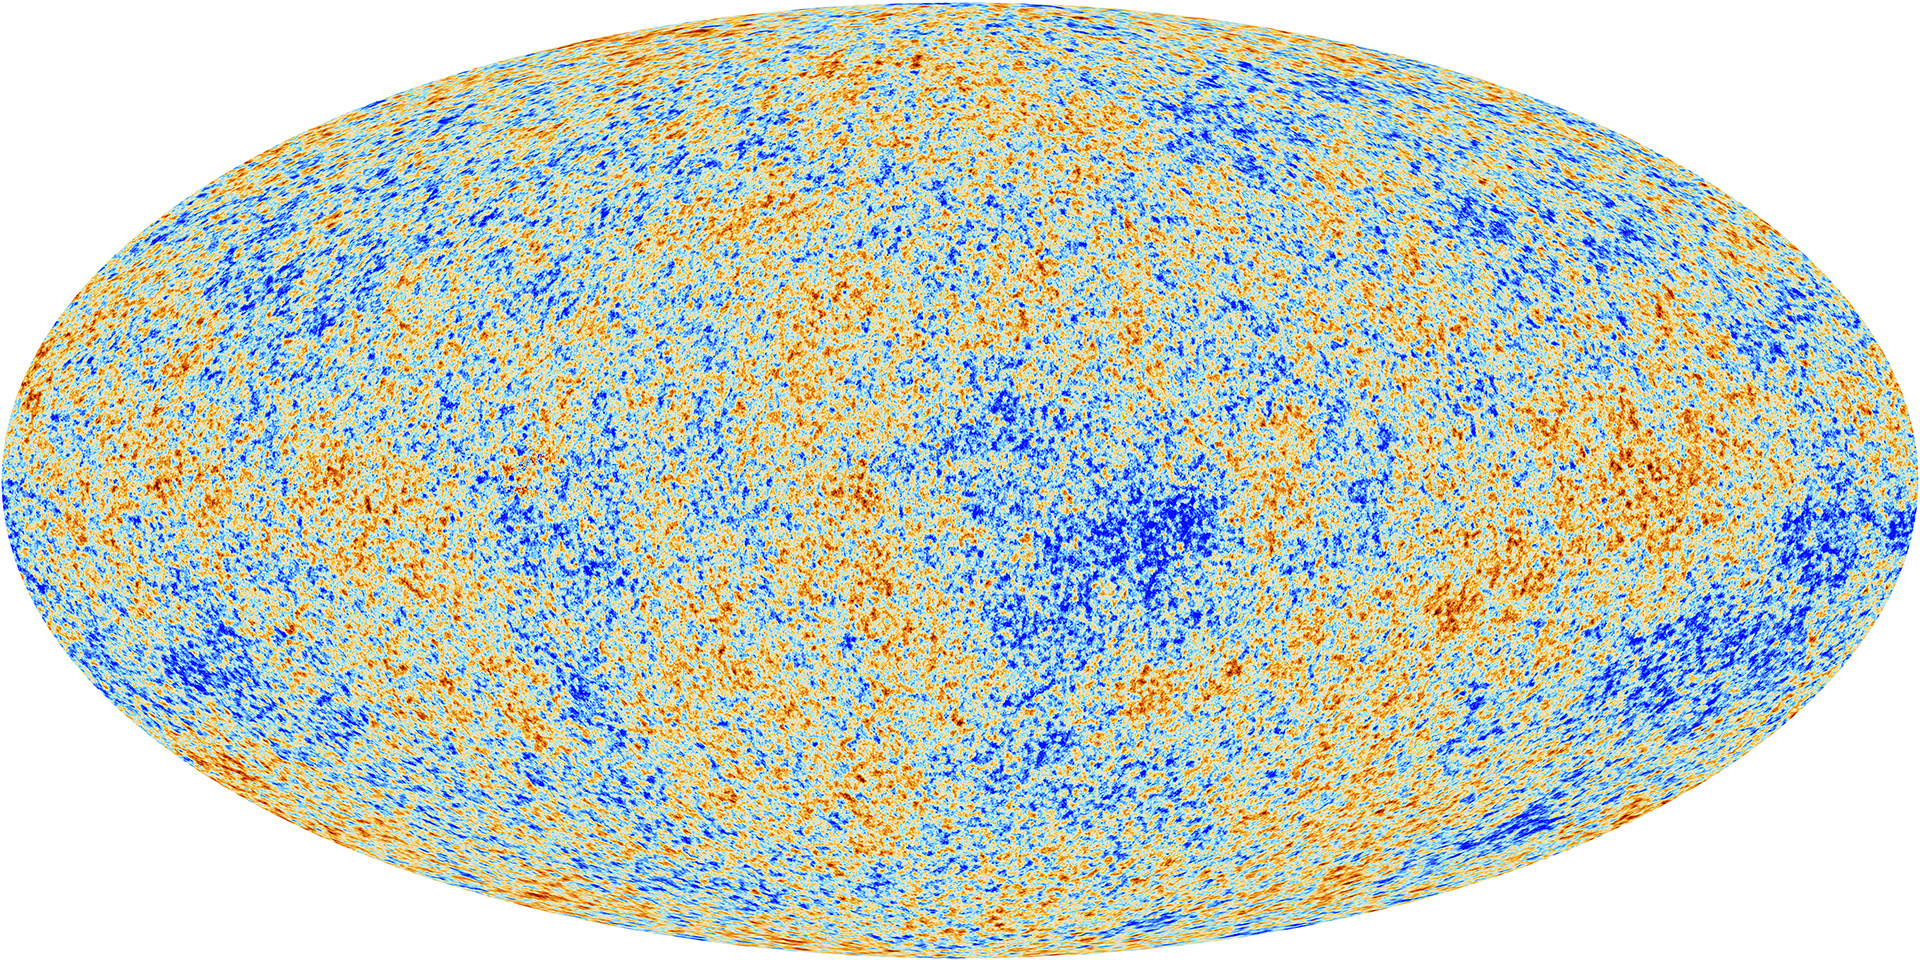
\includegraphics[scale=0.2]{./figures/Planck_CMB.jpg}
	\caption{CMB as captured by PLANCK. Figure taken from Ref.\ \cite{cmb}.}
	\label{fig:cmb}
\end{figure}


\begin{figure}
	\centering
	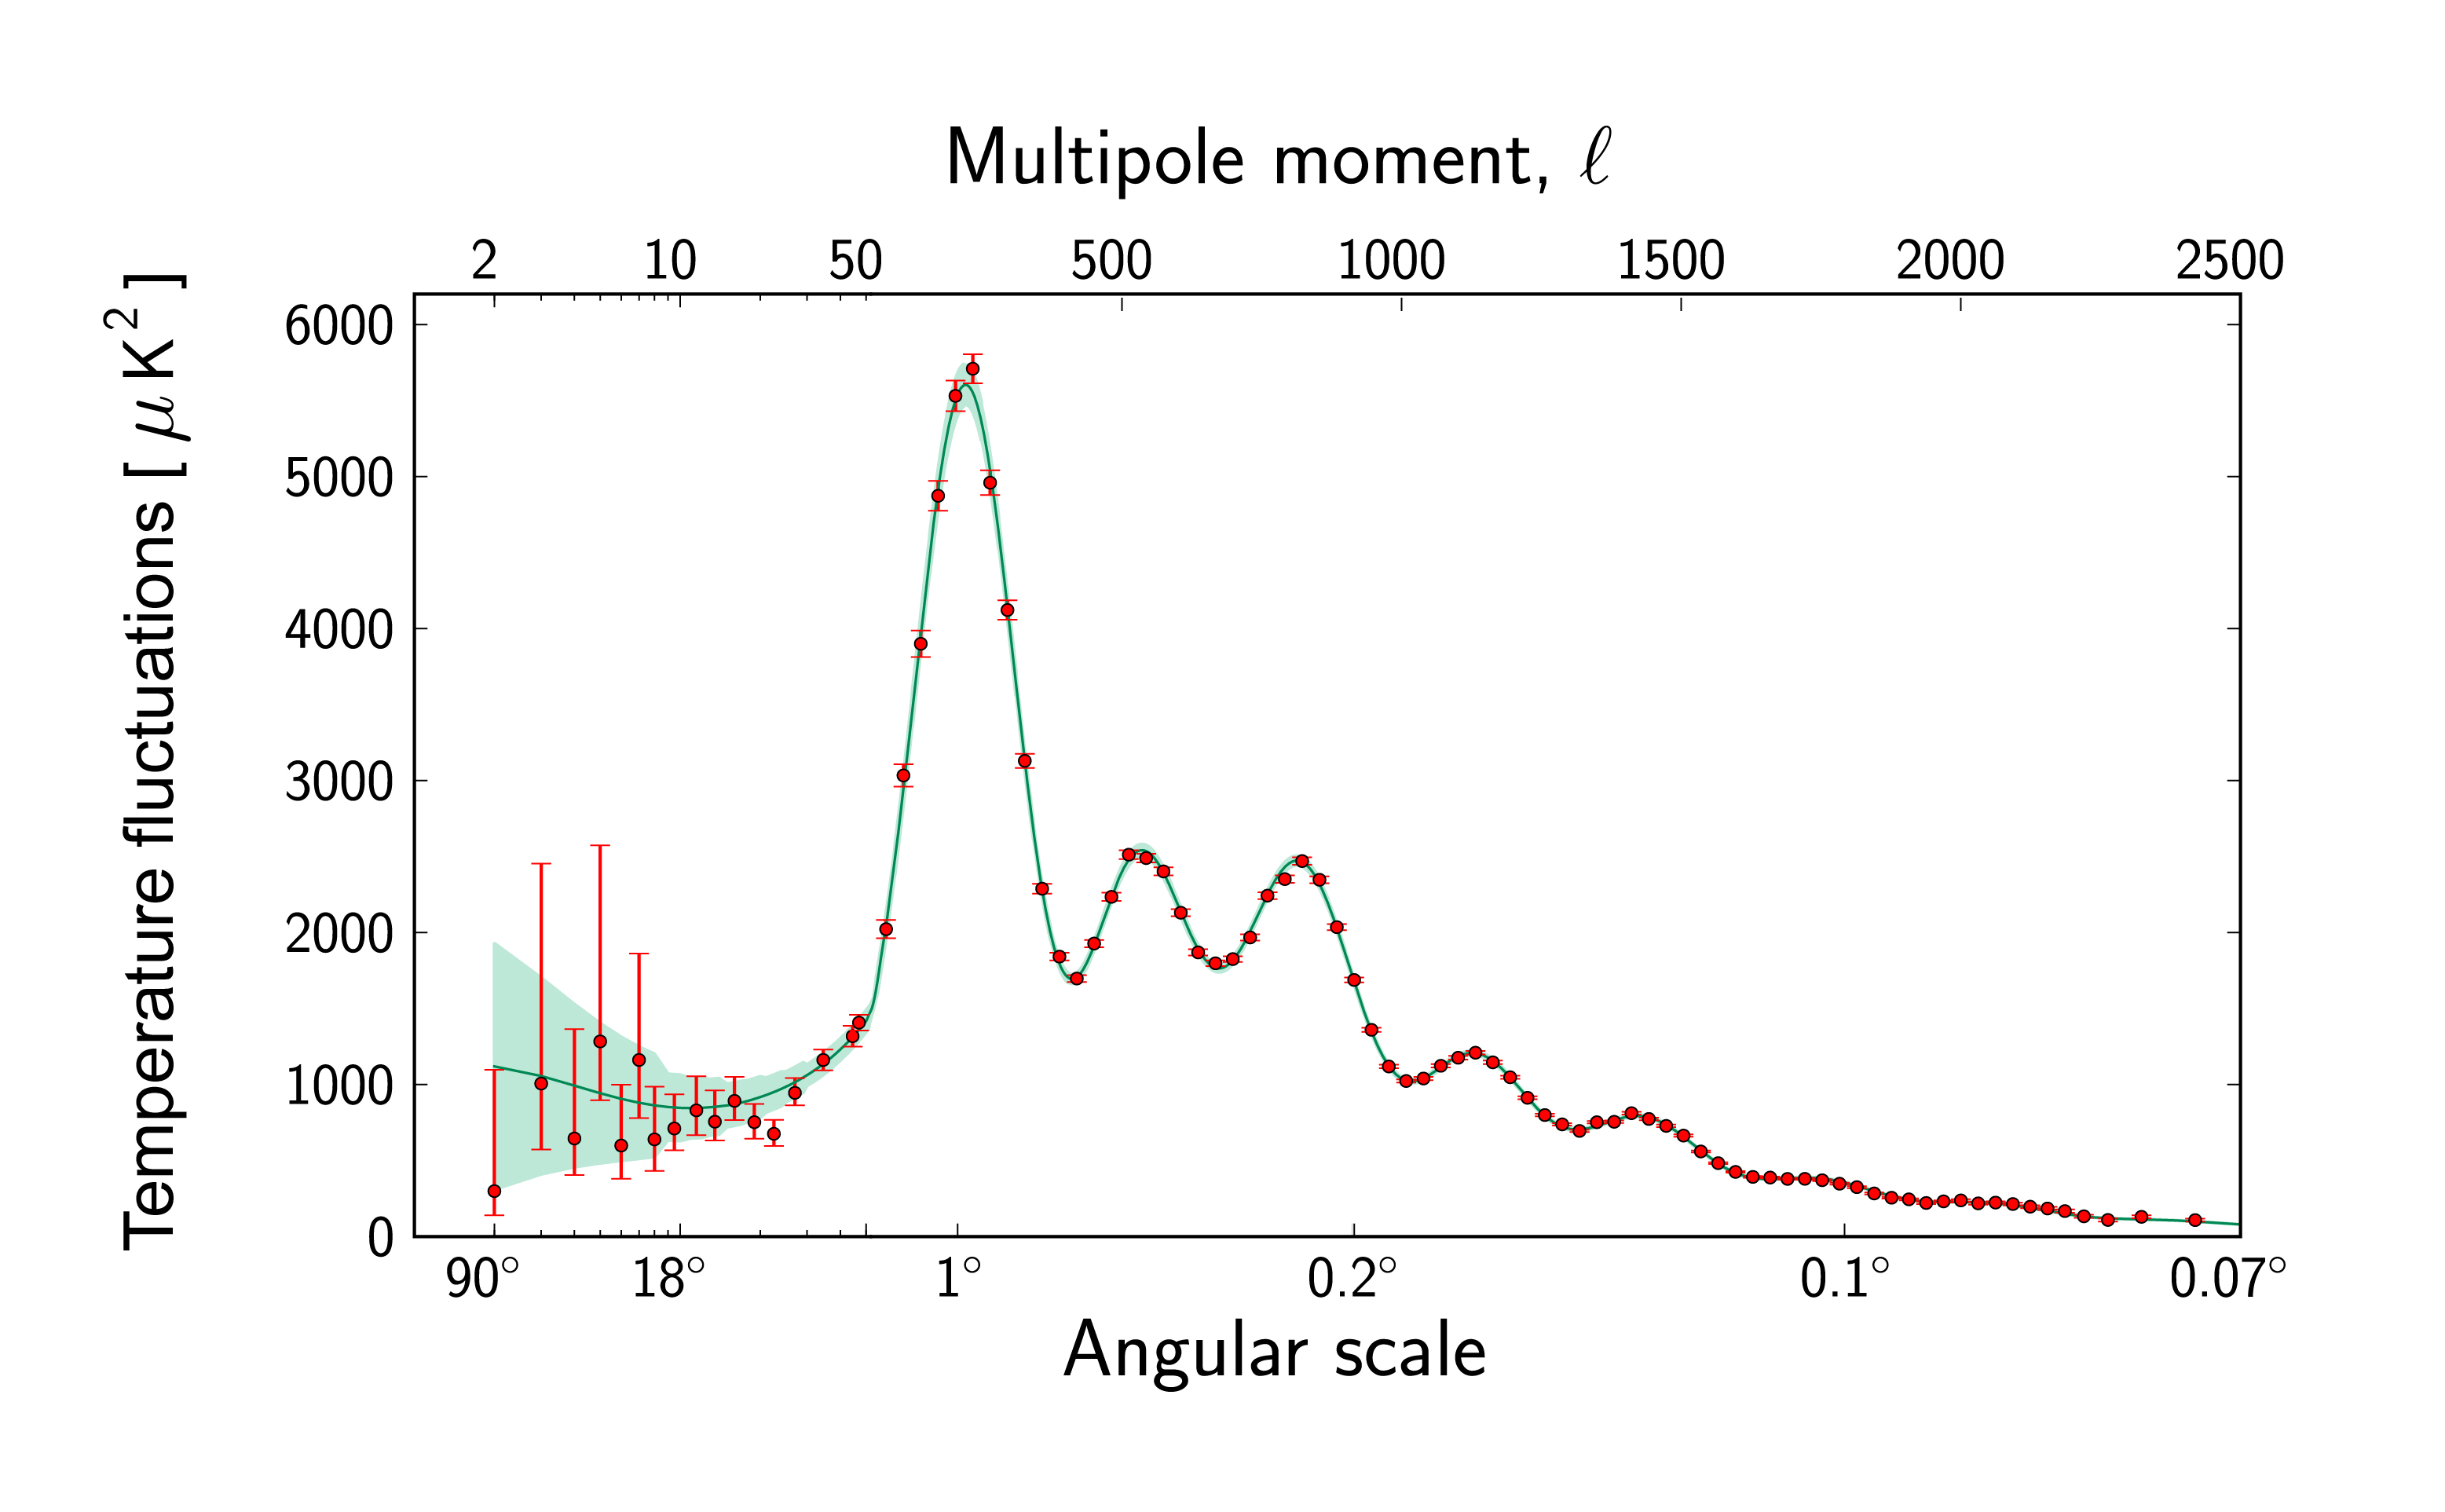
\includegraphics[scale=0.5]{./figures/Planck_Power_Spectrum.jpg}
	\caption{Cosmic Microwave Background power spectrum. Cosmic strings as a seed for large structures is now ruled out, since they do not explain the acoustic peaks at angular scales less than $1^{\circ}$. Plot taken from \cite{powerspec}.}
	\label{fig:powerspec}
\end{figure}



\subsection{Gravitational lensing}
Let us consider a static string along the $z$-axis. In the zero width limit its energy-momentum tensor reads
\begin{equation}
	T^{\mu\nu} = \mu\delta(x)\delta(y)\,\text{diag}(1,0,0,-1).
	\label{eq:energytensor}
\end{equation}
The metric tensor far outside a cosmic string is known to be locally flat, it reads
\begin{equation}
	ds^2 = dt^2-dr'^2-r'^2d\varphi'^2-dz^2,
	\label{eq:metric}
\end{equation}
where $r'$ and $\varphi'$ are defined through the relations 
\begin{equation}
(1-8G\mu\log(r/r_0))r^2 = (1-8G\mu)r^2, \ \ \ \varphi' = (1-4G\mu)\varphi.
\end{equation}
Here $r\in [0,\infty] $ and $\varphi\in[0,2\pi)$ are the usual variables in cylindrical co\-or\-di\-nates and $r_0$ is a constant. This implies that there is an \textit{angular deficit}, which is defined as 
\begin{equation}
\Delta \varphi = \varphi_{\text{max}} - \varphi'_{\text{max}} = 2\pi -2\pi(1-4G\mu) = 8\pi G\mu.
\end{equation}
Physically, it means that a light source, such as a galaxy or a star, behind the core of a string produces a double image separated by the angle 
\begin{equation}
	\alpha = \frac{l_1}{l_2}\Delta\varphi\sin\theta,
\end{equation}
assuming $G\mu\ll 1$, where $l_1$ is the distance between the string and the observer, $l_2$ is the distance between the string and the object and $\theta$ is the angle that the string makes with the plane of the observer and and the object, see Figure \ref{fig:lens}. That is, a non-zero angular deficit suggests that a cosmic string would act as a gravitational lens.

\begin{figure}
	\centering
	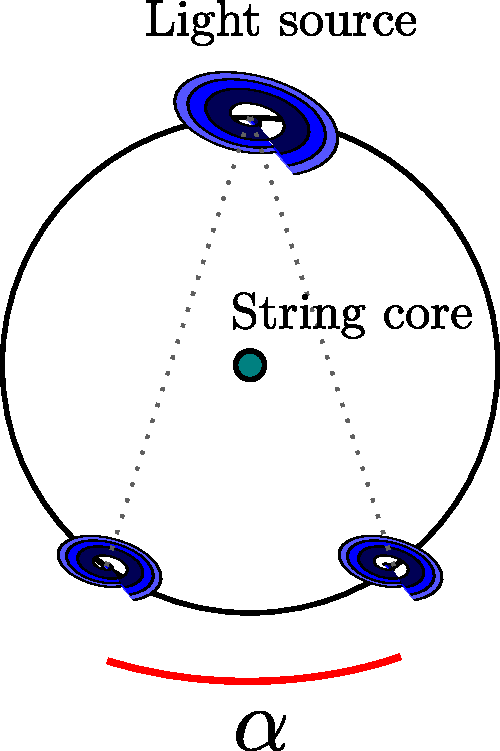
\includegraphics[scale=0.75]{./figures/lens.pdf}
	\caption{Gravitational lensing by a massive cosmic string. An object is behind the string core. The telescopes on Earth would observe two similar close objects separated by the angle $\alpha$.}
	\label{fig:lens}
\end{figure}

For example, we consider an energy scale of $v\sim 10^{16}\ \text{GeV}$, then $G\mu\sim 10^{-6}$, typical of a Grand Unified Theory. A cosmic string, such as one formed due to the spontaneous symmetry breaking of a GUT gauge group, would be very massive and would have a dramatic effect on the lensing of objects behind it. The angular defect of such a string would be $\Delta\varphi = 8\pi G\mu \simeq 5.18''$ \cite{Vilenkin1994}.

 In principle,  an observational way to detect a cosmic string would be to look for a line of double objects. If this is observed, we could conclude that it was caused by a very massive object such as a cosmic string. In Figure \ref{fig:numlens} we see three examples of how a gravitational lens produced by a massive cosmic string would look like, taken from Ref.\ \cite{stringlens}.

\begin{figure}
	\centering
	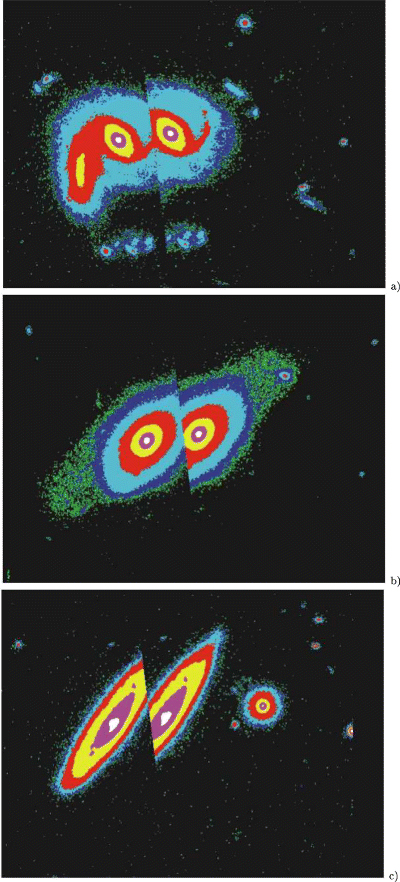
\includegraphics[scale=0.5]{./figures/stringlensing.jpeg}
	\caption{Gravitational lensing by a massive cosmic string generated by numerical simulations, illustration taken from Ref.\ \cite{stringlens}.}
	\label{fig:numlens}
\end{figure} 

In 2003, two close galaxies called CSL-1, see Figure \ref{fig:csl1}, were thought to be two copies of the same galaxy. That is, a gravitational lens produced by a cosmic string, Ref.\ \cite{Sazhin2003}. However, it was ruled out in 2006 by careful measurements on the brightness of the galaxies, see Ref.\ \cite{Agol2006}.

\begin{figure}
	\centering
	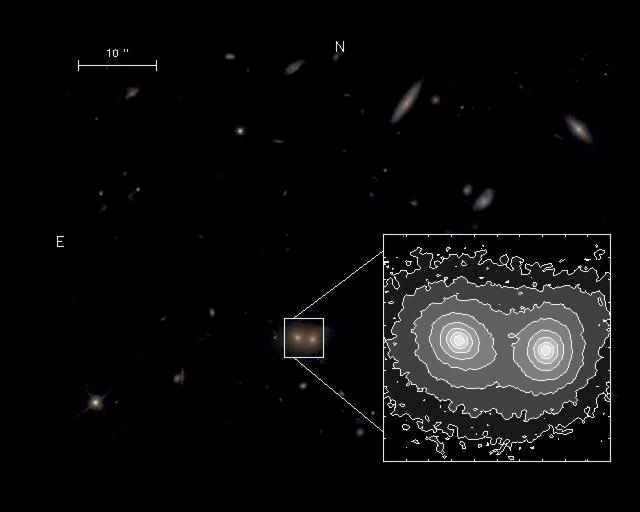
\includegraphics[scale=0.5]{./figures/csl1.jpg}
	\caption{CLS-1 candidate for two copies of the same galaxy as a result of the gravitational lensing of a cosmic string, illustration taken from \cite{Agol2006}.}
	\label{fig:csl1}
\end{figure}
 
 
  Besides gravitational lensing, another gravitational observation would be the detection of gravitational waves.
 
\subsection{Gravitational waves} 

Since the first detection of gravitational waves \cite{PhysRevLett.116.061102}, one of the most realistic way of possible detection of cosmic string is by their emission of gravitational radiation.
According to General Relativity, an oscillating cosmic string loop loose energy by emitting gravitational waves with a power of
\begin{equation}
	P = \Gamma G\mu^2,
\end{equation}
where $\Gamma$ is a constant. 

The production of cosmic string loops can be of various ways, see Figure \ref{fig:loops}. When two strings collide, or when a single string backs on itself, they could form either two new strings, or a new string and a loop. In fact, oscillating loops have a characteristic emission of gravitational radiation produced by \textit{kinks} and \textit{cusps}, through interactions with other strings or with itself. \textit{Kinks} are discontinuities in their worldsheet $x^{\mu}$ or $\dot{x}^{\mu}$. \textit{Cusps} are pointy regions on the string, see Figure \ref{fig:cusp}. A cusp in a loop is formed by two modes, one traveling to the left and the other to the right at the speed of light. Cusps in a loop are short lived and produce a particular signal of gravitational waves beamed in the direction of the cusp. On the other hand, kinks travel along the string and produce a beam of gravitational waves in a fan-like manner.

The Virgo/LIGO Collaboration put constraints on the tension of cosmic strings \cite{PhysRevLett.126.241102}: it found that, referring to loop radiation, the constraint for the tension is
\begin{equation}
	G\mu \lesssim 4\times10^{-15}.
\end{equation}
Unfortunately, this collaboration did not find any evidence of gravitational waves produced by cosmic strings.

\begin{figure}
	\centering
	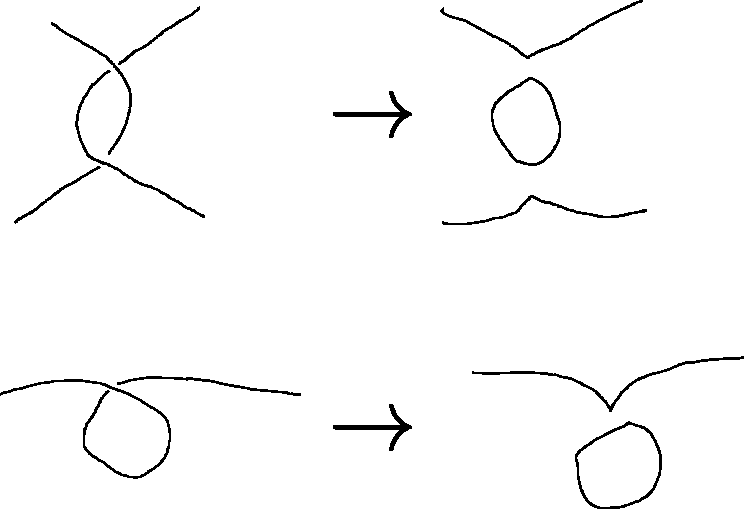
\includegraphics[scale=1]{./figures/kinks.pdf}
	\caption{Formation of loops. Above: two strings intersect and form two new strings and a loop. Below: A string intersects with itself leaving a new string and  a loop. However, the interaction of strings will not always produce loops.}
		\label{fig:loops}
\end{figure}


\begin{figure}
	\centering
	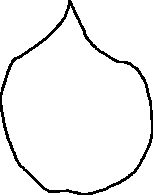
\includegraphics[scale=1.5]{./figures/cusp.pdf}
	\caption{A loop with a cusp. Near the cusp the speeds of the right and left modes are the speed of light.}
		\label{fig:cusp}
\end{figure}

\chapter{U$(1)_{Y'}$ local cosmic strings}\label{chap:Ycosmic}

%\section{Non-existence of cosmic strings in the Standard Model}
%In the Standard Model, the gauge symmetry group is known to be $\text{SU}(3)_c\otimes \text{SU}(2)_L\otimes\text{U}(1)_Y$. If we consider the only scalar field known, the Higgs field $\Phi$, we know that is a field in $\text{SU}(2)_L\otimes\text{U}(1)_Y$ that experience spontaneous symmetry breaking down to $\text{U}(1)_{\text{em}}$. Therefore, the field $\Phi$ takes values in $\left(\text{SU}(2)_L\otimes\text{U}(1)_Y\right)/\text{U}(1)_{\text{em}} \simeq \text{SU(2)}$. Since $\text{SU(2)}\simeq S^3$, we classify their topological defects, and find that $\pi_1(S^3) \simeq I$, therefore no cosmic strings are allowed in the Standard Model. However, extensions to the gauge group of the Standard Model such as SU$(5)$ and effective models can provide a much richer variety of topological defects.

\section{An extension of the Standard Model}
As we saw in Section \ref{sec:globalU}, in the Standard Model U(1)$_{B-L}$ is an exact global symmetry. However, this is strange since an exact symmetry is only natural when it is local. If we promote U(1)$_{B-L}$ to be a local symmetry, we can combine it with the symmetry U$(1)_Y$ of the Standard Model associated with the weak hypercharge $Y$. We introduce an additional U(1) Abelian gauge coupling, and we call it $h'$. We define the new charge as
\begin{equation}
	Y' = 2hY + \frac{h'}{2}(B-L),
\end{equation}
where $h$ and $h'$ are coupling constants (the convention for the coefficients $2$ and $1/2$ will be convenient later). We call the gauge field of the new U$(1)_{Y'}$ symmetry $\mathcal{A}_{\mu}$, it couples to a linear combination of the charges $Y$ and $B-L$.
 
Thus, the gauge group of the Standard Model is converted to 
\begin{equation}
	SU(3)_c\times SU(2)_L\times U(1)_{Y'}.
\end{equation}
%where $h'$ is the coupling of the new gauge boson $\mathcal{A}_{\mu}$.
With the inclusion of the new gauge coupling to $\mathcal{A}_{\mu}$, a gauge anomaly emerges, which can be seen in the triangular diagram in Figure \ref{fig:anomaly}.  In the Standard Model, we have three generations of quarks, each containing two flavors. They can have one of three color charges and be left- or right-handed. Since each quark has baryon number $B=1/3$, each generation sums up to $B = 2\times 3\times 2 \times 1/3 = 4$. 
\begin{figure}
\center
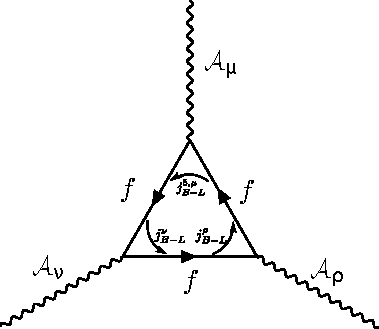
\includegraphics[scale=1]{./figures/triangularanomaly.pdf}
\caption{Triangular diagram: $f$ runs over all fermions involved. In each vertex the quarks of one generation contribute with a total baryon number $B=4$, and the leptons with total lepton number $L=3$. In order to have $\text{U}(1)_{B-L}$ gauge invariance, we introduce a right-handed neutrino with $L=1$ in each fermion generation.}
\label{fig:anomaly}
\end{figure}
In the lepton sector, each generation has one lepton with both chiralities but only a left-handed neutrino, all with $L=1$. This way, each generation contributes to the total lepton number with $L=3$.

This way, the sum of  the $B-L$ charge of one set of SM fermions does not vanish, since $B-L= 4-3=1\neq 0$.

In order to cancel the anomaly, which corresponds to the diagram  in Figure \ref{fig:anomaly}, we need the addition of a right-handed neutrino $\nu_R$ ($L = 1$). Since a right-handed neutrino is sterile, except for the $B-L$ charge, it does not affect the cancellations of other gauge anomalies with respect to the Standard Model gauge fields. It is known that we can give a Dirac mass term to the neutrinos via a Yukawa coupling through $\nu_L$ and $\nu_R$ and the standard Higgs field $\Phi$ of the form
\begin{equation}
f_{\nu} \left[\bar{\nu}_R \begin{pmatrix}-\Phi_0 & \Phi_+\end{pmatrix}\begin{pmatrix}
	\nu_L \\
	e_L
\end{pmatrix} + \begin{pmatrix}\bar{\nu}_L & \bar{e}_L\end{pmatrix}
\begin{pmatrix}
	-\Phi^*_0 \\
	\Phi^*_+
\end{pmatrix}\nu_R\right].
\end{equation}
When we set $\Phi = \begin{pmatrix}0 \\ v \end{pmatrix}$ the mass term becomes $f_{\nu}v(\bar{\nu}_R\nu_L+\bar{\nu}_L\nu_R)$ and we can read directly the mass for the neutrino $m_{\nu} = f_{\nu}v$.

The Majorana term permitted normally to give mass to the right-handed neutrino is of the form
\begin{equation}
	M\bar{\nu}_M \nu_M,
\end{equation}
where $\nu_M = \nu_R + C\bar{\nu}^T_R$, with $C$ the charge conjugation matrix. However, this term is only possible if the right-handed neutrino is completely sterile. We now have a $B-L$ gauge field, and if we want to construct a mass term solely for $\nu_R$, we add a non-standard Higgs field.
 The weak and $B-L$ charges of the Higgs fields are summarize in Table \ref{tab:charges}.
\begin{table}
\begin{center}
\begin{tabular}{|c|c|c|}
\hline 
 Charge & $\chi$ & $\Phi$ \\ 
\hline \hline
$Y$ & 0 & $\frac{1}{2}$ \\ 
\hline 
${B-L}$  & 2 & 0 \\ 
%\hline 
%$Y'={2hY+\frac{h'}{2}(B-L)}$  & $h'$ & $h$ \\ 
\hline 
\end{tabular} 
\end{center}
\caption{The hypercharges of the Higgs fields $\chi$ and $\Phi$.}% and $1/2$, respectively. On the other hand the $B-L$ charge of $\Phi$ is $0$. However, we define the $B-L$ charge of the $\chi$ to be 2 in order to retain gauge invariance.}
\label{tab:charges}
\end{table}

Moreover, we can also give a Majorana-type mass term to $\nu_R$, in\-de\-pend\-ent\-ly of $\nu_L$ through the Higgs mechanism 
\begin{equation}
\label{eq:majorana}
f_{\nu_R} \nu_R^T \chi \nu_R + \text{c.c.},
\end{equation}
where $f_{\nu_R}$ is a Yukawa coupling and in order to retain gauge invariance we added the non-standard Higgs-type field $\chi\in\mathbb{C}$.
The $B-L$ charge of this term must be zero. The neutrino fields together have $B-L = -2$, so the field $\chi$ must have a charge $B-L=2$.

\section{Lagrangian and equations of motion for U(1)$_{Y'}$ cosmic strings} 

The new Higgs field $\chi$ is introduced in the Lagrangian with a gauge invariant potential 
\begin{equation}
V' = \frac{m'^{2}}{2}\chi^*\chi+\frac{\lambda'}{4}(\chi^*\chi)^2.
\end{equation}
Because of power-counting renormalizability we only include four powers in the field $\chi$.
It can be applied to each lepton generation to give mass to all right-handed neutrinos via the Higgs mechanism according to eq.\ \eqref{eq:majorana}. We denote the vacuum expectation value of $\chi$ as $v'$.

It is also natural to include a mixed term $\propto \kappa\Phi^{\dagger}\Phi\chi^*\chi$, between the standard Higgs field and the new Higgs field. This term is natural because it is gauge invariant under both U(1)$_Y'$ and SU$(2)_L$. Again, by power counting renormalizability we only include four powers in energy, giving the coupling constant $\kappa$ dimension zero.

Furthermore, we assume the vacuum expectation value of the new Higgs field $v'$ to be much greater than the vacuum expectation value of the standard Higgs field $v$, that is, $v'\gg v$. In addition, we assume  $f_{\nu_R}\simeq O(1)$ which together gives a heavy mass to the right-handed neutrino, $m_{\nu_R} = f_{\nu_R}v'$. For simplicity, we exclude the SU$(2)_L$ gauge field and the fermion fields, along with the gluons. Therefore, the Lagrangian with these approximations reads
\begin{eqnarray} 
	\mathcal{L} & = & \frac{1}{2}(D^{\mu}\Phi)^{\dagger}D_{\mu}\Phi - \frac{m^2}{2}\Phi^{\dagger}\Phi - \frac{\lambda}{4}(\Phi^{\dagger}\Phi)^2 -\frac{\lambda}{4}v^4   \nonumber\\
 & & +\frac{1}{2}(D^{\mu} \chi)^*D_{\mu} \chi - \frac{m'^2}{2}\chi^*\chi - \frac{\lambda'}{4}(\chi^* \chi)^2 -\frac{\lambda'}{4}v'^4\nonumber \\ 
 & & -\frac{\kappa}{2}\Phi^\dagger\Phi\chi^*\chi  -\frac{\kappa}{2}v^2v'^2 -\frac{1}{4}\mathcal{F}^{\mu\nu}\mathcal{F}_{\mu\nu}, %+ \frac{1}{4}B_{\mu\nu}B_{\mu\nu}
\end{eqnarray}
where 
\begin{eqnarray}
D_{\mu} \Phi & \equiv & (\partial_{\mu} + ih\mathcal{A}_{\mu})\Phi,\nonumber \\ 
D_{\mu} \chi & \equiv & (\partial_{\mu} + ih'\mathcal{A}_{\mu})\chi,\nonumber \\
\mathcal{F}_{\mu\nu} & \equiv & \partial_{\mu}\mathcal{A}_{\nu}-\partial_{\nu}\mathcal{A}_{\mu},
\label{eq:covder}%,\\
%B_{\mu\nu} & = & \partial_{\mu}B_{\nu}-\partial_{\nu}B_{\mu}.
\end{eqnarray}
and the gauge field $\mathcal{A}_{\mu}$ is introduced to implement local U$(1)_{Y'}$ invariance. The fields transform as
\begin{eqnarray}
	\Phi(x) \to e^{ih\alpha(x)}\Phi(x), \nonumber \\
	\chi(x) \to e^{ih'\alpha(x)}\chi(x), \nonumber\\
	\mathcal{A}_{\mu} \to \mathcal{A}_{\mu} + \partial_{\mu} \alpha(x),
\end{eqnarray}
where $\alpha$ is any differentiable function of $x$.
Expanding the covariant derivative terms of eq.\ \eqref{eq:covder} we obtain
\begin{eqnarray*}
	(D^{\mu}\Phi)^{\dagger}D_{\mu}\Phi & = &  \partial^{\mu}\Phi^{\dagger}\partial_{\mu}\Phi + ih\partial^{\mu}\Phi^{\dagger}\mathcal{A}_{\mu} \Phi - ih\mathcal{A}^{\mu} \Phi^{\dagger}\partial_{\mu}\Phi +h^2\mathcal{A}^{\mu}\mathcal{A}_{\mu} \Phi^{\dagger}\Phi,\\
	 (D^{\mu}\chi)^{*}D_{\mu}\chi & = &  \partial^{\mu}\chi^{*}\partial_{\mu}\chi + ih'\partial^{\mu}\chi^{*}\mathcal{A}_{\mu} \chi - ih'\mathcal{A}^{\mu} \chi^{*}\partial_{\mu}\chi +h'^2\mathcal{A}^{\mu}\mathcal{A}_{\mu} \chi^{*}\chi.
\end{eqnarray*}
We want to derive the Euler-Lagrange equations regarding the derivatives with respect to $\Phi^{\dagger}$
\begin{eqnarray}
	\partial^{\mu}\frac{\partial \mathcal{L}}{\partial (\partial^{\mu}\Phi^{\dagger})} & = & \frac{\partial \mathcal{L}}{\partial \Phi^{\dagger}},\nonumber \\
	\frac{\partial  \mathcal{L}}{\partial (\partial^{\mu} \Phi^{\dagger})}  & = & \frac{1}{2}\partial_{\mu} \Phi + \frac{ih}{2}\mathcal{A}_{\mu}\Phi = \frac{1}{2}D_{\mu}\Phi,\nonumber \\
	\label{eq:eula_lhs}
	 \partial^{\mu}\frac{\partial \mathcal{L}}{\partial (\partial^{\mu}\Phi^{\dagger})} & = & \frac{1}{2}\partial^{\mu} \left(\partial_{\mu} + i h\mathcal{A}_{\mu}\right)\Phi = \frac{1}{2}\partial^{\mu}D_{\mu}\Phi,
\end{eqnarray}
\begin{eqnarray}
\label{eq:eula_rhs}
	\frac{\partial \mathcal{L}}{\partial \Phi^{\dagger}}  & = &  \frac{1}{2} \left[-ih\mathcal{A}^{\mu}\partial_{\mu}\Phi + h^2\mathcal{A}^{\mu}\mathcal{A}_{\mu}\Phi \right]- \frac{m^2}{2}\Phi -  \frac{\lambda}{2} (\Phi^{\dagger}\Phi)\Phi - \frac{\kappa}{2}\Phi \chi^*\chi\nonumber\\
	& = &-\frac{1}{2}ih\mathcal{A}^{\mu}D_{\mu} \Phi - \frac{m^2}{2}\Phi - \frac{\lambda}{2}  (\Phi^{\dagger}\Phi)\Phi - \frac{\kappa}{2}\Phi \chi^*\chi \ .
\end{eqnarray}
Equating \eqref{eq:eula_lhs} and \eqref{eq:eula_rhs} we obtain the equation of motion for $\Phi$
\begin{equation}
	\label{eq:phi}
	D^{\mu}D_{\mu} \Phi = -m^2 \Phi - \lambda (\Phi^{\dagger}\Phi)\Phi - \kappa \Phi \chi^* \chi \ .
\end{equation}
Similarly, we obtain the equation of motion for the field $\chi$
\begin{equation}
	\label{eq:chi}
	D^{\mu}D_{\mu} \chi = -m'^2 \chi - \lambda' (\chi^{*}\chi)\chi - \kappa \chi \Phi^{\dagger} \Phi \ . 
\end{equation}
Regarding the equations of motion of the gauge field $\mathcal{A}_{\mu}$, we first take the derivate of the Lagrangian with respect to $\mathcal{A}_{\rho}$
\begin{eqnarray}
	\frac{\partial \mathcal{L}}{\partial \mathcal{A}_{\rho}} & = & \frac{ih}{2}\partial^{\rho}\Phi^{\dagger}\Phi -\frac{ih}{2}\Phi^{\dagger}\partial^{\rho}
	 \Phi+h^2\mathcal{A}^{\rho}\Phi^{\dagger}\Phi\nonumber\\
	 & & + \frac{ih'}{2}\partial^{\rho}\chi^{*}\chi -\frac{ih'}{2}\chi^{*}\partial^{\rho}\chi+h'^2\mathcal{A}^{\rho}\chi^{*}\chi \nonumber\\
	& = & \frac{ih}{2}\left[ (D^{\rho}\Phi)^{\dagger}\Phi-\Phi^{\dagger}D^{\rho}\Phi\right] + \frac{ih'}{2}\left[ (D^{\rho}\chi)^{*}\chi-\chi^{*}D^{\rho}\chi\right].
\end{eqnarray}
Then, we take the derivative of the Lagrangian with respect to $\partial_{\lambda}\mathcal{A}_{\rho}$ 
\begin{eqnarray}
	\label{eq:maxwell}
	\frac{\partial \mathcal{L}}{\partial (\partial_{\lambda}\mathcal{A}_{\rho})} & = & \frac{\partial}{\partial (\partial_{\lambda}\mathcal{A}_{\rho})}\left(-\frac{1}{4}\mathcal{F}^{\mu\nu}\mathcal{F}_{\mu\nu}\right) \nonumber\\
	& = & -\frac{1}{4}\frac{\partial}{\partial (\partial_{\lambda}\mathcal{A}_{\rho})}\left(\partial^{\mu}\mathcal{A}^{\nu}-\partial^{\nu}\mathcal{A}^{\mu}\right)\left(\partial_{\mu}\mathcal{A}_{\nu}-\partial_{\nu}\mathcal{A}_{\mu}\right) \nonumber\\
	& = & -\frac{1}{4}\frac{\partial}{\partial (\partial_{\lambda}\mathcal{A}_{\rho})}(2\partial^{\mu}\mathcal{A}^{\nu}\partial_{\mu}\mathcal{A}_{\nu}-2\partial^{\mu}\mathcal{A}^{\nu}\partial_{\nu}\mathcal{A}_{\mu}) \nonumber\\
	& = & -\frac{1}{4}\left(2\partial^{\mu}\mathcal{A}^{\nu}\delta_{\lambda\mu}\delta_{\rho\nu}-2\partial^{\mu}\mathcal{A}^{\nu}\delta_{\lambda\nu}\delta_{\rho\mu}-2\partial^{\nu}\mathcal{A}^{\mu} \delta_{\lambda\mu}\delta_{\rho\nu}+2\partial^{\nu}\mathcal{A}^{\mu}\delta_{\lambda\nu}\delta_{\rho\mu}\right) \nonumber\\
	& = & -\frac{1}{4}(4\partial^{\lambda}\mathcal{A}^{\rho}-4\partial^{\rho}\mathcal{A}^{\lambda}) = -\partial^{\lambda}\mathcal{A}^{\rho}+\partial^{\rho}\mathcal{A}^{\lambda} = -\mathcal{F}^{\lambda\rho} = \mathcal{F}^{\rho\lambda}.
\end{eqnarray}
Differentiating the result of eq.\ \eqref{eq:maxwell} by $x_{\lambda}$ yields
\begin{equation}
\partial_{\lambda}\left(\frac{\partial \mathcal{L}}{\partial (\partial_{\lambda}\mathcal{A}_{\rho})}\right) = \partial_{\lambda}\mathcal{F}^{\rho\lambda} = \partial_{\lambda}\partial^{\rho}\mathcal{A}^{\lambda}-\partial_{\lambda}\partial^{\lambda}\mathcal{A}^{\rho}.
\end{equation}
Thus, we obtain the equations of motion  for the gauge field $\mathcal{A}_{\mu}$
\begin{equation}
\label{eq:max_eqs}
\partial_{\lambda}\mathcal{F}^{\rho\lambda} = \frac{ih}{2}\left[ (D^{\rho}\Phi)^{\dagger}\Phi-\Phi^{\dagger}(D^{\rho}\Phi)\right] + \frac{ih'}{2}\left[ (D^{\rho}\chi)^{*}\chi-\chi^{*}(D^{\rho}\chi)\right].
\end{equation}
Using cylindrical coordinates $(r,\varphi,z)$, we make ans\"{a}tze for the stationary solutions 
\begin{equation}
\Phi = \begin{pmatrix} 0 \\
  \phi(r)e^{in\varphi}\end{pmatrix},
   \ \ \ \chi = \xi(r) e^{in'\varphi}, \ \ \ \mathcal{A}^{\varphi}= \frac{a(r)}{r}.
\end{equation}
 Then, the $\varphi$ components of the covariant derivatives are
\begin{eqnarray}
	\frac{1}{r}D_{\varphi}\Phi = \left(\frac{1}{r}\partial_{\varphi} + ih\mathcal{A}_{\varphi}\right)\Phi, \nonumber \\
	 \frac{1}{r}D_{\varphi}\chi = \left(\frac{1}{r}\partial_{\varphi} + ih'\mathcal{A}_{\varphi}\right)\chi ,
\end{eqnarray}
along with
\begin{eqnarray}
	D^iD_i \Phi\equiv \left(\partial_r^2 + \frac{1}{r}\partial_r +\left(\frac{1}{r}\partial_{\varphi}+ih\mathcal{A}_{\varphi}\right)^2 +\partial^2_z\right)\Phi, \nonumber \\
	D^iD_i \chi\equiv \left(\partial_r^2 + \frac{1}{r}\partial_r +\left(\frac{1}{r}\partial_{\varphi}+ih'\mathcal{A}_{\varphi}\right)^2 +\partial^2_z\right)\chi \ .
\end{eqnarray}
%\begin{eqnarray}
%	\left(\frac{1}{r}\partial_{\varphi}+ih\frac{a(r)}{r}\right)^2\phi e^{in\varphi} %& = & \left(\frac{1}{r}\partial_{\varphi}+ih\frac{a(r)}{r}\right)\left(\frac{1}{r}\partial_{\varphi}+ih\frac{a(r)}{r}\right)\phi e^{in\varphi} \\
%	& = & \left(\frac{1}{r}\partial_{\varphi}+ih\frac{a(r)}{r}\right)\left(\frac{1}{r}(in)\phi e^{in\varphi} +ih \frac{a(r)}{r}\phi e^{in\varphi} \right) \\
%	& = & \left(\frac{1}{r^2}(in)^2\phi e^{in\varphi}+2(in)ih \frac{a(r)}{r^2}\phi e^{in\varphi}-h^2\frac{a(r)^2}{r^2}\phi e^{in\varphi}\right) \\
%	& = & -\left(\frac{n^2}{r^2}+2nh\frac{a(r)}{r^2}+h^2\frac{a(r)^2}{r^2}\right)\phi e^{in\varphi} \\
%	\left(\frac{1}{r}\partial_{\varphi}+ih'\frac{a(r)}{r}\right)^2\xi e^{in'\varphi} & = & -\left(\frac{n'^2}{r^2}+2n'h'\frac{a(r)}{r^2}+h'^2\frac{a(r)^2}{r^2}\right)\xi e^{in'\varphi} 
%\end{eqnarray}
We now work out the left-hand side of eq.\ \eqref{eq:max_eqs}, for static configurations
\begin{eqnarray}
\label{eq:vec_rel_max}
	\partial_{\nu}\mathcal{F}^{\mu\nu}  & = & \partial_{\nu} \partial^{\mu}\mathcal{A}^{\nu}-\partial_{\nu}\partial^{\nu}\mathcal{A}^{\mu} =-\partial_j\partial^i\mathcal{A}^j+\partial^j\partial_j\mathcal{A}^i \nonumber \\
	 & = &  -\left[\nabla(\nabla\cdot \mathcal{A})\right]^i+\left[ \nabla^2 \mathcal{A}\right]^i\nonumber \\
	 & = & - \left[\nabla\times\nabla\times\mathcal{A}\right]^i.
	%&    \frac{\partial_r^2 a}{r}-\frac{\partial_r a}{r^2} \ .
\end{eqnarray}
In cylindrical coordinates, the curl of a vector function takes the form of the determinant \cite{Arfken}
\begin{equation}
	\nabla\times\vec{b} = \frac{1}{r}\begin{vmatrix}
	\hat{r} & r{\hat{\varphi}} & \hat{z} \\
	\partial_r & \partial_{\varphi} & \partial_z \\
	b^r & rb^{\varphi} & b^z 
	\end{vmatrix}.
\end{equation}
Then
\begin{eqnarray}
	\nabla\times\vec{\mathcal{A}} = \nabla\times\left( \frac{a(r)}{r}\hat{\varphi}\right) & = & \frac{1}{r} \begin{vmatrix}
	\hat{r} & r\hat{\varphi} & \hat{z} \\
	\partial_r & \partial_{\varphi} & \partial_z \\
	0 & a & 0
	\end{vmatrix} = \frac{1}{r}\partial_r a \ \hat{z}, \nonumber \quad\\
	\nabla \times \nabla \times \vec{\mathcal{A}} = \nabla \times \left(\frac{1}{r}\partial_r a \ \hat{z}\right) & = & \frac{1}{r}\begin{vmatrix}
	\hat{r} & r\hat{\varphi} & \hat{z} \\
	\partial_r & \partial_{\varphi} & \partial_z \\
	\label{eq:rel1}
	0 & 0 & \frac{1}{r}\partial_r a 
	\end{vmatrix}\nonumber \\
	& = & \left(-\frac{1}{r}\partial_r^2 a + \frac{1}{r^2}\partial_r a\right)\hat{\varphi} \quad
\end{eqnarray}
Eq. \eqref{eq:vec_rel_max} is non-trivial only for the index $j = \varphi$, where we obtain from eq.\ \eqref{eq:rel1}
\begin{equation}
	\label{eq:max_eqs_phi}
	\partial_j\mathcal{F}^{\varphi j} = \frac{1}{r}\partial_r^2 a - \frac{1}{r^2}\partial_r a.
\end{equation}
Now we treat the terms on the right-hand side of eq.\ \eqref{eq:max_eqs},
\begin{eqnarray}
%\label{eq:first_rel}
\frac{ih}{2}\left(\frac{1}{r}\partial_{\varphi}\Phi\right)^{\dagger}\Phi = \frac{ih}{2}\frac{1}{r}\partial_{\varphi}(\phi e^{-in\varphi})\phi e^{in\varphi} = \frac{hn}{2r}\phi^2 \nonumber \\ 
-\frac{ih}{2}\Phi^{\dagger}\left(\frac{1}{r}\partial_{\varphi}\Phi\right) = -\frac{ih}{2}\frac{1}{r}\partial_{\varphi}(\phi e^{in\varphi})\phi e^{-in\varphi} = \frac{hn}{2r}\phi^2 \nonumber \\
h^2 \mathcal{A}_{\varphi} \Phi^{\dagger}\Phi = h^2\frac{a}{r}\phi e^{-in\varphi}\phi e^{in\varphi} = h^2 \frac{a}{r}\phi^2 \nonumber \\
\frac{ih'}{2}\left(\frac{1}{r}\partial_{\varphi}\chi\right)^{*}\chi = \frac{ih'}{2}\frac{1}{r}\partial_{\varphi}(\xi e^{-in'\varphi})\xi e^{in'\varphi} = \frac{h'}{2} n'\frac{1}{r}\xi^2  \nonumber \\ 
-\frac{ih'}{2}\chi^{*}\left(\frac{1}{r}\partial_{\varphi}\chi\right) = -\frac{ih'}{2}\frac{1}{r}\partial_{\varphi}(\xi e^{in'\varphi})\xi e^{-in'\varphi} =\frac{h'}{2} n'\frac{1}{r}\xi^2\nonumber  \\
\label{eq:last_rel}
h'^2 \mathcal{A}_{\varphi} \chi^{*}\chi = h'^2\frac{a}{r}\xi e^{-in'\varphi}\xi e^{in'\varphi} = h'^2\frac{a}{r}\xi^2 \ .
\end{eqnarray}


From eq.\ \eqref{eq:phi} we infer the equation of motion for $\phi(r)$
\begin{equation}
	\label{eq:final_phi}
	\partial_r^2 \phi + \frac{1}{r} \partial_r \phi- \frac{1}{r^2}\left(n+ha\right)^2\phi- m^2 \phi- \lambda \phi^3-\kappa \phi \xi^2 = 0,
\end{equation}
and from eq.\ \eqref{eq:chi} we obtain
\begin{equation}
	\label{eq:final_xi}
	\partial_r^2 \xi + \frac{1}{r} \partial_r \xi - \frac{1}{r^2}\left(n'+h'a \right)^2\xi -m'^2\xi - \lambda' \xi^3 - \kappa \xi \phi^2 = 0\ .
\end{equation}
And finally from eqs.\ \eqref{eq:max_eqs_phi} and \eqref{eq:last_rel} we infer
\begin{equation}
	\label{eq:a}
\partial_r^2a -\frac{1}{r}\partial_r a-h(n+ha)\phi^2-h' (n'+h'a)\xi^2 = 0.
\end{equation}
\subsection{Boundary conditions}
In the limit $r\to \infty$, the radial profile functions $\phi$ and $\xi$ take constant values $v$ and $v'$, respectively. In the same limit, eqs.\ \eqref{eq:final_phi} and \eqref{eq:final_xi} fix the values for $m^2$ and $m'^2$. If we treat $\lambda$, $\lambda'$ and $\kappa$ as free parameters, we fix the values for $m^2$ and $m'^2$
\begin{eqnarray}
	\label{eq:meqs}
	-m^2v-\lambda v^3 - \kappa v v'^2 = 0 & \Rightarrow & m^2 = -\kappa v'^2 - \lambda v^2, \nonumber\\
	-m'^2v'-\lambda' v'^3 - \kappa v' v^2 = 0 & \Rightarrow  & m'^2 = -\kappa v^2 - \lambda' v'^2.
\end{eqnarray}
Also the value $a(r\to\infty)$ is fixed using eq.\ \eqref{eq:a}. We are interested in solutions that apply to any values of $\phi$ and $\xi$ which is only possible when the parentheses in eq.\ \eqref{eq:a} are zero in the limit $r\to\infty$. We obtain the limit
\begin{equation}
\lim_{r\to \infty}a(r) \equiv a(\infty) = -\frac{n}{h}=-\frac{n'}{h'}.
\label{eq:goodlimit}
\end{equation} 
In addition, there exists another limit of $a$ at infinity
%\begin{equation}
%\partial_r^2a -\frac{1}{r}\partial_r a-h(n+ha)\phi^2-h' (n'+h'a)\xi^2 = 0
%\end{equation}
%so at $r\to \infty$, the value of $a$ is fixed only if we have
\begin{equation}
	-hnv^2 - h^2a(\infty)v^2 - h' n' v'^2 - h'^2 a(\infty) v'^2 = 0 \ \ \Rightarrow  \ \ a(\infty) = -\frac{hnv^2+h'n' v'^2}{h^2v^2+h'^2 v'^2}.
	\label{eq:badlimit}
\end{equation}
We reject the limit in eq.\ \eqref{eq:badlimit} because we demand the function $a$ to be independent of $v$ and $v'$. In contrast, the limit of \eqref{eq:goodlimit} is valid for any $\phi$ and $\xi$ which are constant at $r\to\infty$.


In summary, the boundary conditions for $\phi$, $\xi$, $a$ and  for $n,\ n' > 0$ are 
\begin{eqnarray}
	\phi(0)=0, & \displaystyle\lim_{r\to\infty}\phi(r) = v \nonumber \\
	 \xi(0)=0, &  \displaystyle\lim_{r\to\infty}\xi(r) = v' \nonumber  \\
	 a(0)=0, & \displaystyle \lim_{r\to\infty}a(r) = -\frac{n}{h}=-\frac{n'}{h'}\ .
\end{eqnarray}
For $n=0$ or $n'=0$, $\phi(0)\neq 0$ or $\xi(0) \neq 0$ is possible, respectively.

\subsection{Condition on $\kappa$}

We know that for the potential to be bounded from below, the constants $\lambda$ and $\lambda'$ must be both positive.

We now study the conditions on the Higgs-Higgs coupling $\kappa$. The potential term involving the Higgs fields is
\begin{equation}
V(\Phi,\chi) = \frac{m^2}{2}\Phi^{\dagger}\Phi+\frac{m'^2}{2}\chi^{*}\chi+\frac{\lambda}{4}(\Phi^{\dagger}\Phi)^2+\frac{\lambda'}{4}(\chi^{*}\chi)^2+\frac{\kappa}{2}\Phi^{\dagger}\Phi\chi\chi^*,
\end{equation}
where $m^2<0$ and $m'^2<0$.

To take a general perspective, it is convenient to study the concavity of the function
\begin{equation}
V(x,y) = ax^2 + by^2+cx^4+dy^4+ex^2y^2
\end{equation}
where $a,b<0$ and $c,d>0$. However, if we demand $V$ to be bounded from below it is not sufficient that $c,d>0$; we need a condition for $e$. The Hessian matrix of $V(x,y)$ reads
$$H=\begin{pmatrix}
2a+12cx^2+2ey^2 & 4exy \\
4exy & 2b+12dy^2+2ex^2 
\end{pmatrix},$$
and the gradient is
$$\nabla V = \begin{pmatrix}
2ax+4cx^3+2exy^2 \\
2by+4dy^3+2ex^2y
\end{pmatrix}.$$
From the gradient we note that the point $(0,0)$ is a critical point of $V$. At this point the Hessian takes the form
$$H(0,0)=\begin{pmatrix}
2a & 0 \\
0 & 2b
\end{pmatrix}.$$
Since the eigenvalues of $H$ at $(0,0)$ are both negative, we know that the function $V$ is concave, hence $(0,0)$ is a local maximum.
There are other critical points: those points must be local minima or saddle points for $V$ since we demand $V$ to be bounded from below and we already found the only local maximum. In order to study them, we perform the coordinate transformation
\begin{equation}
	X = x^2, \ \ \ \ Y =y^2.
	\label{eq:changeofcoor}
\end{equation}
The potential becomes
\begin{equation}
V(X,Y) = aX + bY+cX^2+dY^2+eXY.
\end{equation}
The gradient is zero when 
\begin{eqnarray}
2cX + eY & = & -a \\
eX + 2dY & = & -b
\end{eqnarray}
with the solution
\begin{eqnarray}
X_c & = & \frac{-2ad+be}{4cd-e^2}, \\
Y_c & = & \frac{-2bc+ae}{4cd-e^2}.
\end{eqnarray}
The Hessian matrix of $V$ for this coordinate transformation, evaluated at this critical point, is
\begin{equation}
H=\begin{pmatrix}
2c & e \\
e & 2d
\end{pmatrix}.
\end{equation}
Focusing on the local minima of the function, we know that in this case $\det H>0$ and $\frac{\partial^2 V}{\partial X^2} = 2c > 0$, see \cite{Marsden2012}. Due to eq.\ \eqref{eq:changeofcoor} both $X_c$ and $Y_c$ are positive quantities, and since the determinant is positive for the minima, that means that the numerators are also positive, which implies
\begin{equation}
	e<\frac{2ad}{b} ,\ \ \ e<\frac{2bc}{a},
\end{equation}
and
\begin{equation}
	\det H = 4cd - e^2 > 0 \ \ \ \Rightarrow  \ \ \ e^2 < 4cd.
\end{equation}
If we substitute
$$a = \frac{m^2}{2}, \ \ \  b = \frac{m'^2}{2}, \ \ \  c = \frac{\lambda}{4}, \ \ \  d = \frac{\lambda'}{4}, \ \ \ e = \frac{\kappa}{2},$$
then we have conditions on $\kappa$
\begin{equation}
-\sqrt{\lambda \lambda'} < \kappa < \sqrt{\lambda \lambda'},
\end{equation}
and
\begin{equation}
	{\kappa} < \frac{m^2\lambda'}{m'^2}, \ \ \ {\kappa} < \frac{m'^2\lambda}{m^2}.
	\label{eq:redundant}
\end{equation}
We combine all the conditions as follows
\begin{equation}
	-\sqrt{\lambda \lambda'} < \kappa < \min \left(\sqrt{\lambda \lambda'},\frac{m'^2\lambda}{m^2},\frac{m^2\lambda'}{m'^2}\right).
\end{equation}
However, the inequalities in eq.\ \eqref{eq:redundant} are redundant. We take the values for $m^2$ and $m'^2$ from eq.\ \eqref{eq:meqs} and substitute them in one of the inequalities. Working with the first one in  eq.\ \eqref{eq:redundant} and recalling that $m^2,\ m'^2 <0$, we obtain
\begin{eqnarray}
	{\kappa} & < & \frac{-\kappa v'^2 - \lambda v^2}{-\kappa v^2 - \lambda' v'^2}\lambda'\nonumber \\
	& = & \frac{\kappa v'^2 + \lambda v^2}{\kappa v^2 + \lambda' v'^2}\lambda' \nonumber \\
	\kappa^2v^2+\kappa\lambda' v'^2 & < & \kappa\lambda' v'^2 + \lambda\lambda' v^2 \nonumber\\
	\kappa^2 & < & \lambda\lambda'. 
\end{eqnarray}
Similarly, we obtain the same result when we work out the second inequality in eq.\ \eqref{eq:redundant}. We are left with only one condition
\begin{equation}
 \boxed{\kappa^2 < \lambda \lambda'}\ .
\end{equation}


%Figures \ref{fig:1}, \ref{fig:2}, \ref{fig:3} and \ref{fig:4} show the solutions for the functions $\phi$, $\xi$ and $a$ for various values of $n$, $n'$, $h$, $h'$, $\lambda$, $\lambda'$ in the range $\kappa\in[-2,2]$ and $\kappa\in[-1.5,1.5]$ for figure \ref{fig:3}. 
%
%
%\begin{figure}
%\centering
%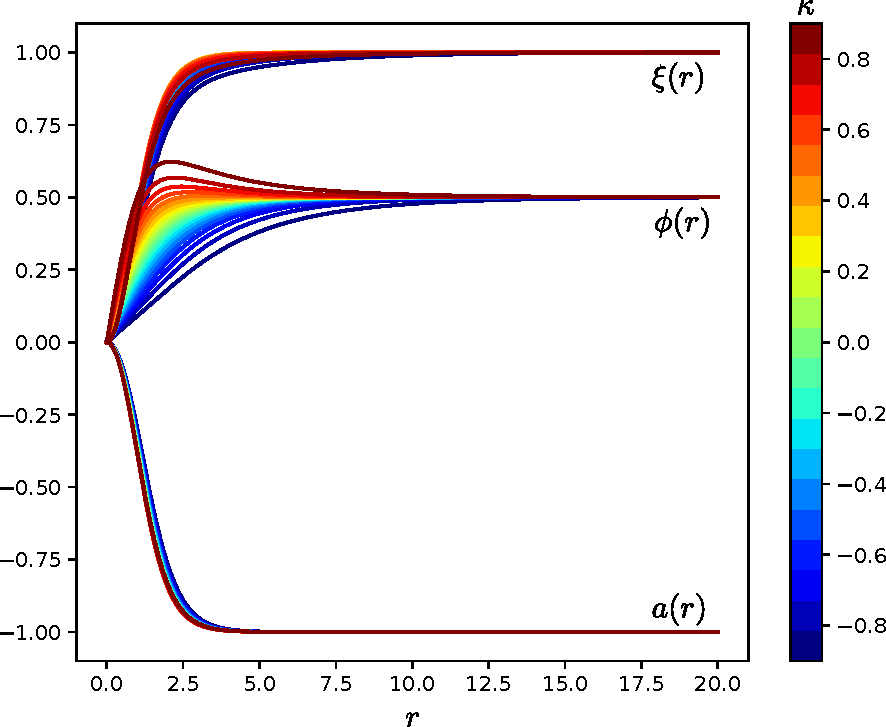
\includegraphics[scale=1]{./figures/Figure_1.pdf}
%\caption{$h=n=0$, $h'=n' = 1$, $\lambda=\lambda'=1$, $v=0.1$, $v'=1/4$ and $\kappa\in [-2,2]$.}
%\label{fig:1}
%\end{figure}
%
%\begin{figure}
%\centering
%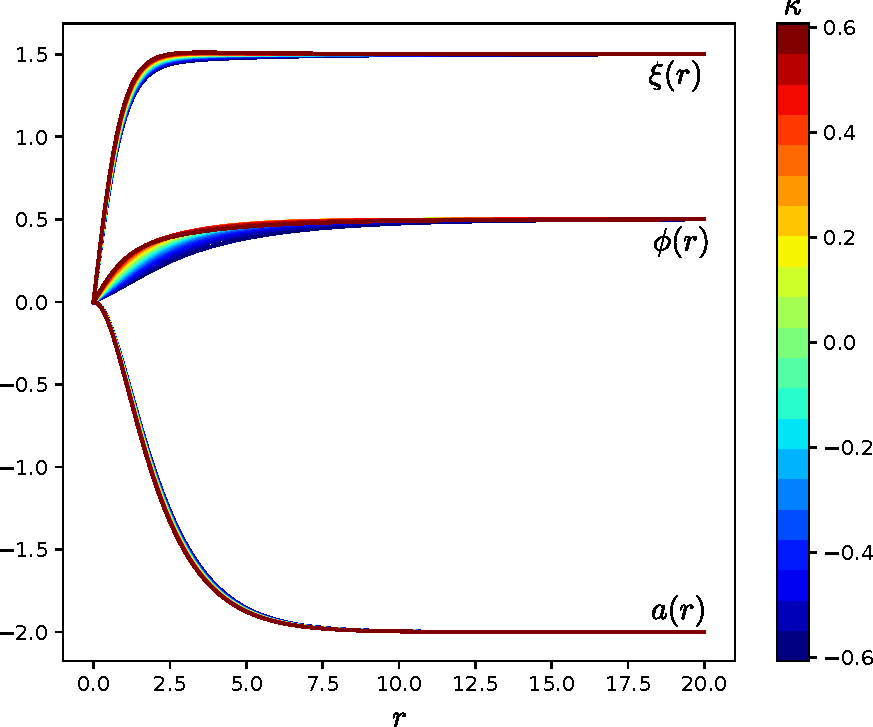
\includegraphics[scale=1]{./figures/Figure_2.pdf}
%\caption{$h=n=0$, $h'=n' = 1$, $\lambda=\lambda'=1$, $v=1/2$, $v'=1$ and $\kappa\in [-2,2]$.}
%\label{fig:2}
%\end{figure}
%
%\begin{figure}
%\centering
%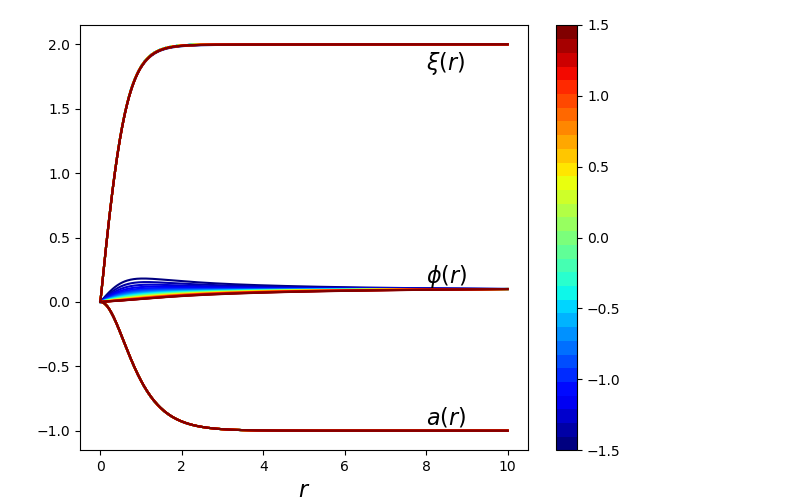
\includegraphics[scale=1]{./figures/Figure_3.png}
%\caption{$h=n=1$, $h'=n' = 1$, $\lambda=1, \lambda'=1/4$, $v=0.1$, $v'=2$ and $\kappa\in [-1.5,1.5]$.}
%\label{fig:3}
%\end{figure}
%
%\begin{figure}
%\centering
%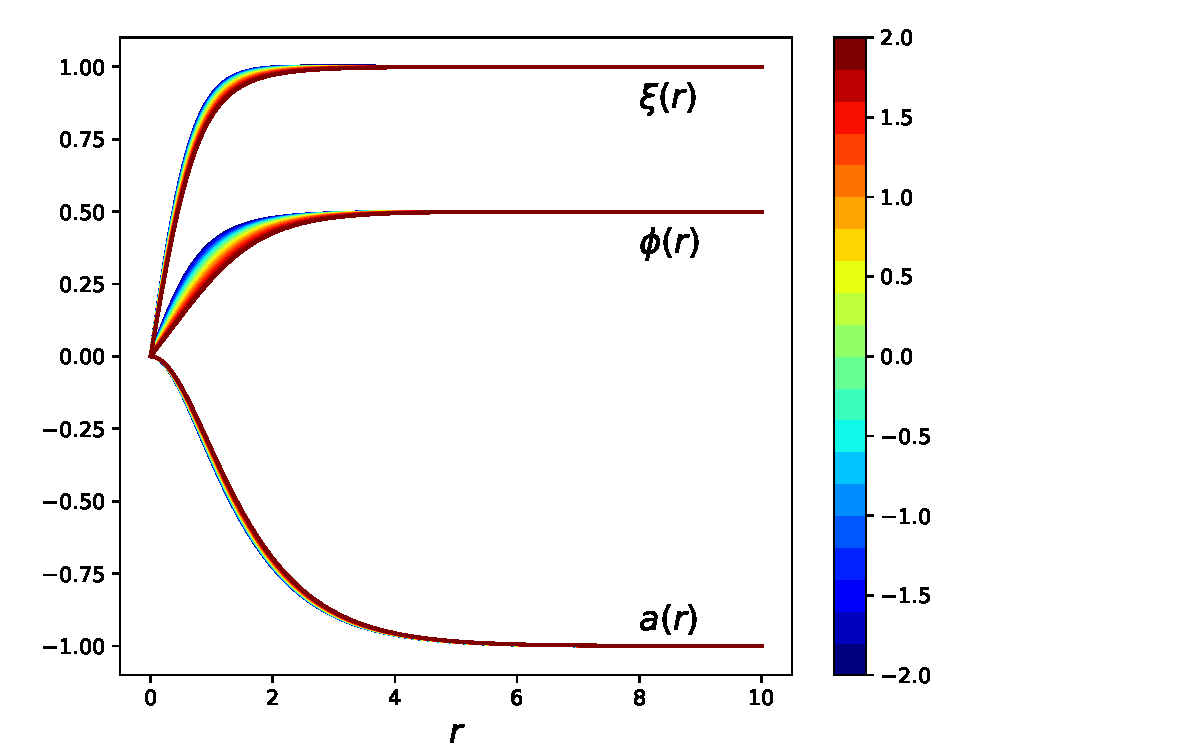
\includegraphics[scale=1]{./figures/Figure_4.pdf}
%\caption{$h=n=1$, $h'=n' = 1$, $\lambda=\lambda'=1$, $v=1/2$, $v'=1$ and $\kappa\in [-2,2]$.}
%\label{fig:4}
%\end{figure}


\chapter{Profiles of U$(1)_{Y'}$ cosmic strings}\label{chap:results} 
In order to explore the profile of the string, we solve the non-linear system of second order differential equations for the fields $\phi$, $\xi$ and $a$, 
\begin{equation}
	\partial_r^2 \phi + \frac{1}{r} \partial_r \phi- \frac{1}{r^2}\left(n^2+2nha+h^2a^2\right)\phi- m^2 \phi- \lambda \phi^3-\kappa \phi \xi^2 = 0,
\end{equation}
\begin{equation}
	\partial_r^2 \xi + \frac{1}{r} \partial_r \xi - \frac{1}{r^2}\left(n'^2+2n'h' a+h'^2a^2 \right)\xi -m'^2\xi - \lambda' \xi^3 - \kappa \xi \phi^2 = 0 ,
\end{equation}
\begin{equation}
	\partial_r^2a -\frac{1}{r}\partial_r a-hn\phi^2-h^2a\phi^2-h' n'\xi^2 - h'^2 a \xi^2 = 0.  
\end{equation}
When $n,n'\neq 0$, they are subject to the boundary conditions, derived in Chapter 3,
\begin{eqnarray}
	\phi(0)=0, & \displaystyle\lim_{r\to\infty}\phi(r) = v, \nonumber \\
	 \xi(0)=0, &  \displaystyle\lim_{r\to\infty}\xi(r) = v', \nonumber  \\
	 a(0)=0, & \displaystyle \lim_{r\to\infty}a(r) = -\frac{n}{h}=-\frac{n'}{h'},
\end{eqnarray}
and
\begin{align}
	\label{eq:constraints}
	\lambda>0, \ \ \ \lambda'>0, \ \ \ \kappa^2 < \lambda \lambda',\nonumber \\
	 m^2 = -\kappa v'^2 - \lambda v^2<0,\ \ \ m'^2 = -\kappa v^2 - \lambda' v'^2<0. 
\end{align}

The solutions to the boundary value problem are obtained numerically by the Python function \texttt{scipy.integrate.solve\_bvp} which applies the damped Newton method.
The Newton method is a procedure of solving systems of ordinary differential equations where an initial guess is generated and subsequent iterations of the method give, ideally,  better ap\-prox\-i\-ma\-tions to the solution.

Let us take a vector function $\vec{f}(\vec{x})$ and let $\vec{x}^*$ be a root, i.e.\ $\vec{f}(\vec{x}^*)=0$. If we choose an initial guess $\vec{x}_0$ for the root, the method gives a sequence of approximations $\vec{x}_{1},\, \vec{x}_{2},\dots,\, \vec{x}_{n+1}$ by solving the system of equations
\begin{equation}
	J(\vec{x}_n)\vec{\xi} = - \vec{f}(\vec{x}_n), 
\end{equation}
where $J(\vec{x}_n)$ is the Jacobian matrix and the Newton direction $\vec{\xi}$ is defined through $\vec{x}_{n+1} = \vec{x}_{n}+\vec{\xi}$.
An ap\-prox\-i\-ma\-tion is generated by the previous one in the Newton direction. The length of the Newton direction is called the step size. In some situations, the Newton step size is too large, so we require it to be smaller. The idea of the damped Newton method is to modify the length of the Newton step size in order to have better convergence in some situations. Thus, we modify the solution by
\begin{equation}
	\vec{x}_{n+1} = \vec{x}_{n} + \lambda\vec{\xi}, \ \ \ 0<\lambda\leq 1.
\end{equation} 
See Ref.\ \cite{Ascher} for a complete review on this topic.

 A solution is uniquely defined by inputting the values for the Higgs expectation values $v$, $v'$, the self-coupling constants $\lambda$, $\lambda'$, the Higgs fields interaction term $\kappa$, the coupling constants $h$, $h'$ and finally the winding numbers $n$ and $n'$ subject to the constraints in eq.\ \eqref{eq:constraints}. We choose $v'>v$ in order to have a heavier $\chi$ boson than the standard Higgs field $\Phi$. Also, $v=246$ GeV is used to convert all quantities into physical units.  For instance, lengths are converted into physical units through
\begin{equation}
	r_{\text{physical}} = r_{\text{dimensionless}} \ \ \frac{v_{\text{dimensionless}}}{246 \ \text{GeV}} \ \ 0.197 \ \text{GeV} \ \text{fm}.
\end{equation}

Figure \ref{fig:fig1} shows the case $n=n'=h=h'=\lambda=\lambda'=1$, $v = 0.5$, $v'=1$ (in units where $v=246$ GeV) and $-1<\kappa<1$. We see the typical profile behavior of cosmic strings. Approximately at $r \gtrsim 7.5$ which corresponds to  $0.003\ \text{fm}$, the field profiles attain their asymptotic vacuum expectation values. Solutions for positive values of $\kappa$ tend to stay closer to each other under variation  of $\kappa$ than the ones with $\kappa<0$, which spread out when $\kappa$ approaches its minimum $\kappa\to-\sqrt{\lambda\lambda'}$.

Figure \ref{fig:fig2} shows the case where $n=h=\lambda=\lambda'=1$, $n'=h'=2$, $v=0.5$, $v'=1$. We consider a higher winding number $n'$ than in the previous case and we see interesting features. We observe that the standard Higgs field exceeds, or overshoots, its vacuum expectation value at large $r$. This is an interesting phenomenon not reported in the literature.  Physically, it means that a particle passing close to the string could temporarily acquire a greater mass than far from it.
The solutions to the function $\phi$ appear to be spread out when $\kappa^2\to \lambda\lambda'$, and denser when $\kappa\to 0$. The solutions to the function $\xi$ overlap, suggesting that there exist at least two equal or very similar solutions, one with $\kappa>0$ and the other with a negative $\kappa$.%, where $\kappa\approx 0$. 

%Similar interpretations to solutions in figs.\ \ref{fig:fig3} and .
In Figure \ref{fig:fig3} we change the parameters to $n=n'=1,\ \lambda=0.5,\  \lambda'=1$, $n'=h'=0.5$, $v=0.5$, $v'=1$. We see a milder effect of the spreading of the solutions of the functions $\phi$ and $\xi$ and no overshooting.

In Figure \ref{fig:fig4} the parameters are $n=h=\lambda=\lambda'=1$, $n'=2,\ h'=1$, $v=0.5$, $v'=1.5$. We see again the overshoot of the function $\phi$, which can be associated to a greater winding number of the non-standard Higgs field, $n'>n$. % However, the peak of $\xi$ is not as high as the case in fig.\ \ref{fig:fig2}, which we associate to smaller values of the gauge couplings $h$ and $h'$.

The opposite of the previous cases appears when $n<n'$ and $h>h'$. Now the field that overshoots its vacuum expectation value is $\xi$. This means that when a right-handed neutrino passes near the string core it will acquire a greater mass than far from the string. In Figure \ref{fig:n-5h5np-1hp1l1lp1v05vp2} we see a mild overshoot in the $\xi$ function, and a overlap in the function $\phi$, in addition, a mild overlap of $a$ is visible. We also see a plateau of $\phi$ around zero, this is because the expansion of the function around the origin is proportional to $r^{|n|}$, as we saw in Chapter \ref{chap:back}.


We can include our model into a larger gauge group. According to Ref.\ \cite{Fritzsch75}, our model is embedded into the group SO(10), a Grand Unification Theory, actually the most popular since SU(5) has been ruled out. Ref.\ \cite{BUCHMULLER1991395} investigates a gauge group embedded in SO(10), namely, the gauge group $\text{SU}(3)_c\times \text{SU}(2)_L\times\text{U}(1)_Y \times \text{U}(1)_{Y'}$. The model is an extension of the Standard Model where a neutral vector boson $Z'$ is added. 
Here the non-standard hypercharge takes the form
\begin{equation}
	\label{eq:refhypercharge}
	Y' = Y - \frac{5}{4}(B-L),
\end{equation}
in contrast to the form of our hypercharge $Y'$
\begin{equation}
	Y' = 2hY - \frac{h'}{2}(B-L).
\end{equation}
Equation \eqref{eq:refhypercharge} constrains the values for the gauge couplings, so they become $h = 1/2$ and $h'= -5/2$. This also implies a condition on the winding numbers, as anticipated in eq.\ \eqref{eq:goodlimit},
\begin{equation}
	n' = -5n.
\end{equation}
We do not discuss at depth this model, we only give numerical solutions for this particular case where the gauge couplings are held fixed.

In Figure \ref{fig:fig5} with $n=1,\ n'=-5,\ h=1/2,\ h'=5/2,\ \lambda=\lambda'=1$, $v = 0.5$, $v'=1$ and $-1<\kappa<1$, we see a dramatic overshoot of the field $\phi$ when $r\sim 2.5$, it reaches almost the double of its vacuum expectation value at $r\to\infty$. However, the behavior of the function $a(r)$ does not change significantly in comparison to the previous cases. 

Figure \ref{fig:fig6} with $n=-2,\ n'=10,\ h=1/2,\ h'=-5/2,\ \lambda=\lambda'=1$, $v = 0.5$, $v'=1$ is another example within the SO(10) model. Again, the overshoot of $\phi$ is clearly visible. Here, the function $\xi$ has a flat part around zero, since the function is proportional to $r^{|n|}$, as we saw in eq.\ \eqref{eq:fapproxsol}. We add that solutions with high winding numbers can hardly be stable. 

In Refs.\ \cite{victor2022} and \cite{bietenholz2022} similar plots were reported, however they did not observe the coaxial behavior of some solutions. In the limit $v\ll v'$ and $n < n'$, we observed coaxial string solutions in the profile of $\phi$. Figure \ref{fig:coaxial} with $n=-2,\ n'=10,\ h=1/2,\ h'=-5/2,\ \lambda=\lambda'=1$, $v = 0.01$, $v'=1$, the parameters are the same as in the previous case but with a different $v$. We observe an overshoot when $\kappa \simeq 0.25$ and when $\kappa$ is grater than this value, the solution has a coaxial behavior. A coaxial solution is negative at low $r$, passes the $r$-axis, and then approaches its positive vacuum expectation value. According to Ref.\ \cite{bogo1975}, for only one Higgs field with $|n|>1$ and $2\lambda/h^2 > 1$, the interpretation of the coaxial solution is that the cosmic string is not stable. 

We also plot the energy density of the function in Figure \ref{fig:edencoaxial}. In the case $v'\gg v$, we expect a tension of the string of the order of $v'^2$. In this case $v' = 100v$, and we expect a tension of the order of $10^9 \ \text{GeV}^2$. In fact, integrating numerically the energy density, we obtain a tension $\mu$ near $1.2\times 10^{10}\ \text{GeV}^2$ for all $\kappa$-values. And its gravitational coupling is approximately
\begin{equation}
	G\mu \approx 8.3\times 10^{-29}.
\end{equation}

 This type of cosmic string with the length of an horizon would have a mass of $\sim 10^{25}$ kg, equivalent to the mass of the Earth, or five orders of magnitude smaller that the mass of the Sun. The small gravitational coupling makes it very difficult for gravitational detection, like gravitational waves or gravitational lensing. However, they are not rule out by constraints in the tension from current data.

\begin{figure}
	\centering
	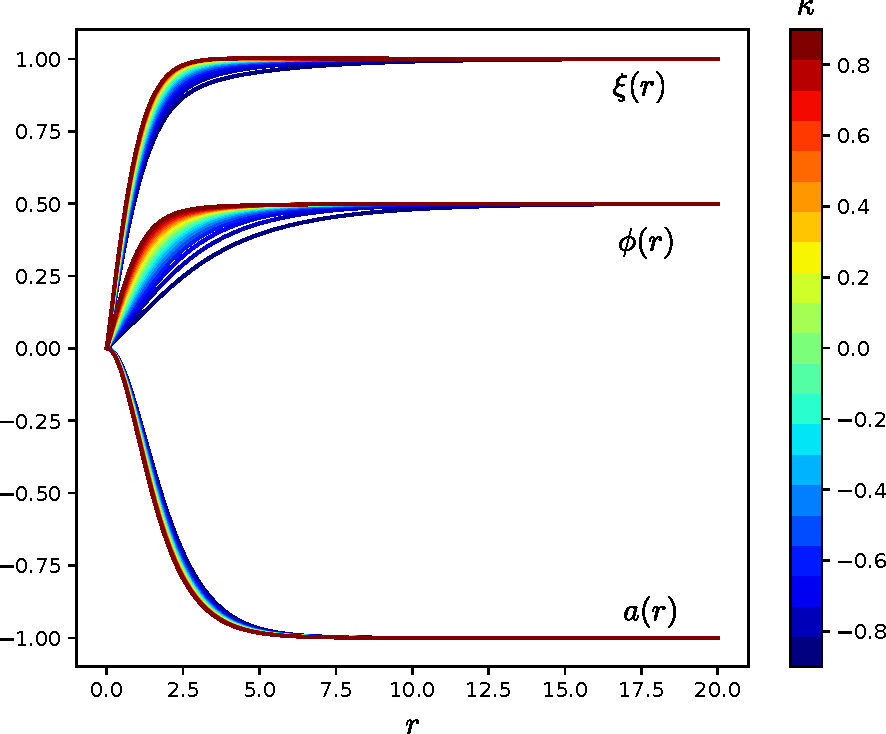
\includegraphics[scale=1]{./figures/F0.pdf}
	\caption{Solutions for the cosmic string profile functions with $v = 0.5$, $v'=1$, $n=n'=h=h'=\lambda=\lambda'=1$. Solutions with $\kappa>0$ tend to stay closer to each other, in contrast to solutions when $\kappa<0$, that spread out $\kappa$ is varied.}
	\label{fig:fig1}
\end{figure}


\begin{figure}
	\centering
	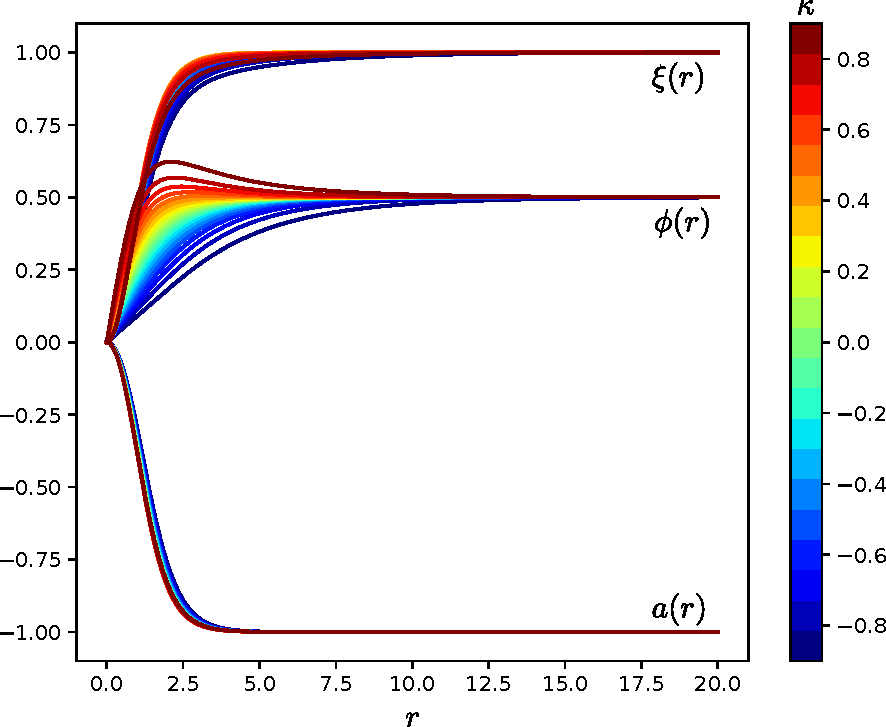
\includegraphics[scale=1]{./figures/Figure_1.pdf}
	\caption{Solutions for the cosmic string profile functions with $v = 0.5$, $v'=1$, $n=1$, $n'=2$, $h=1$, $h'=2$, $\lambda=\lambda'=1$. A lump in the profile of $\Phi$ is present. This behavior is not reported in the literature. Physically, a particle passing near the string core could acquire a greater mass than far from the string. Solution for $\xi$ overlap, which suggests that there exist very similar solutions, one with $\kappa>0$ and one with $\kappa < 0$.}
	\label{fig:fig2}
\end{figure}

\begin{figure}
	\centering
	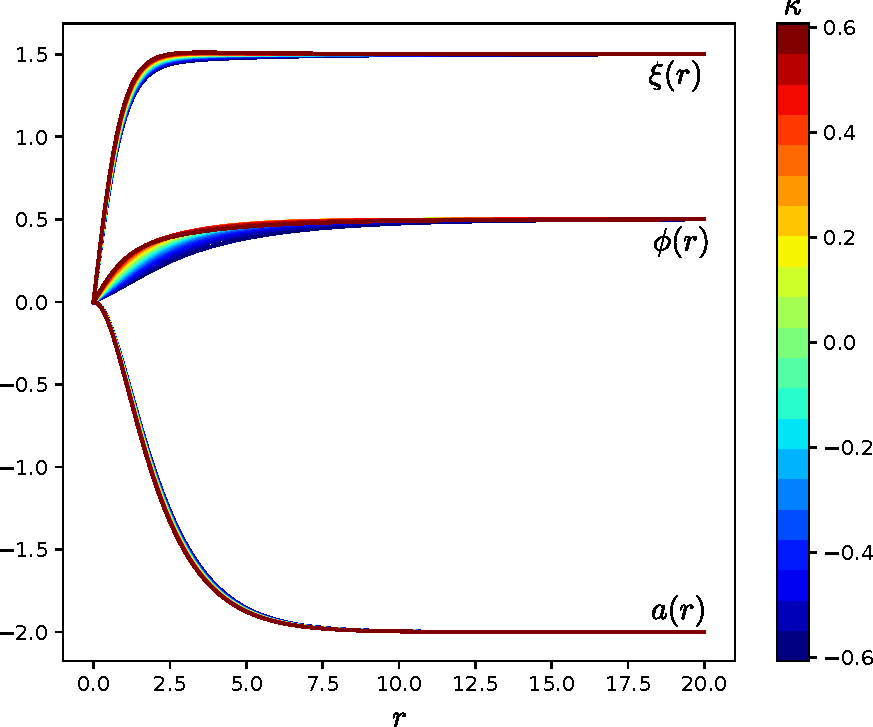
\includegraphics[scale=1]{./figures/Figure_2.pdf}
	\caption{Solutions for the cosmic string profile functions with $v = 0.5$, $v'=1$, $n=1$, $n'=1$, $h=0.5$, $h'=0.5$, $\lambda=0.5,$ $\lambda'=1$. A modest effect of the spreading in the solutions for $\phi$ is observed.}
	\label{fig:fig3}
\end{figure}


\begin{figure}
	\centering
	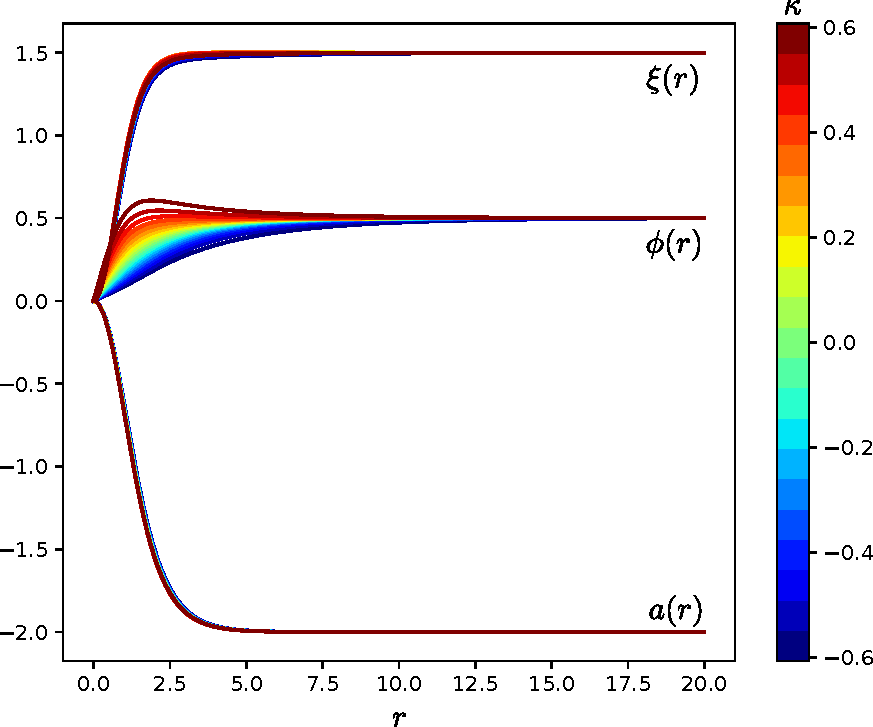
\includegraphics[scale=1]{./figures/Figure_3.pdf}
	\caption{Solutions for the cosmic string profile functions with $v = 0.5$, $v'=1$, $n=1$, $n'= 2$, $h=0.5$, $h'=1$, $\lambda=0.5,\lambda'=1$.  A lump in the profile of $\Phi$ is present. This behavior is not reported in the literature. Physically, a particle passing near the string core could acquire temporarily a greater mass than far from the string.}
	\label{fig:fig4}
\end{figure}

\begin{figure}
	\centering
	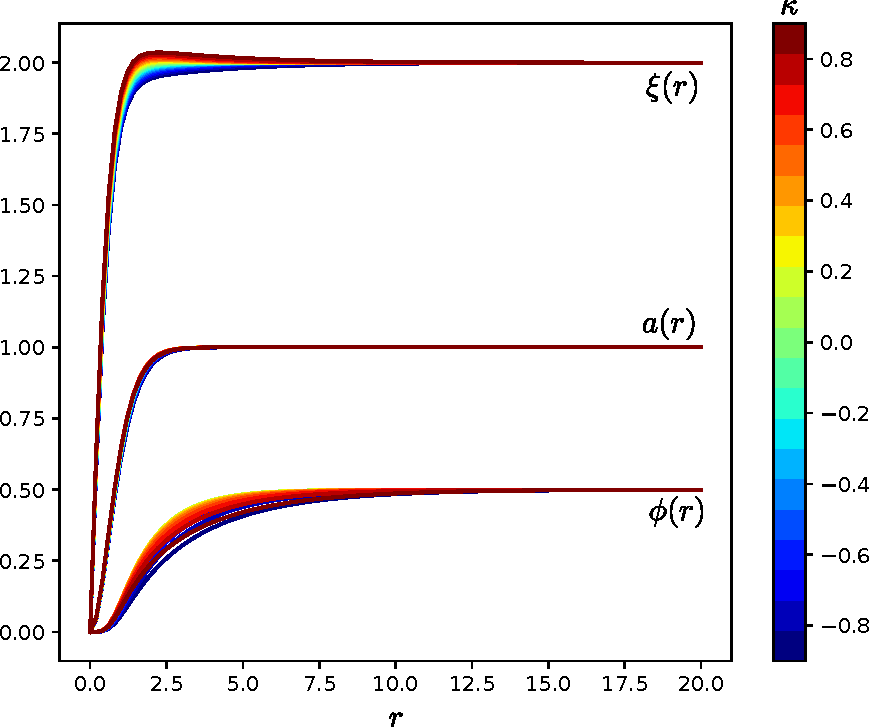
\includegraphics[scale=1]{./figures/n-5h5np-1hp1l1lp1v05vp2.pdf}
	\caption{Solutions for the cosmic string profile functions with $v = 0.5$, $v'=2$, $n=-5$, $n'=-1$, $h=5$, $h'=1$, $\lambda=\lambda'=1$. A lump in the profile of $\chi$ is present. Physically, a right-handed neutrino passing near the string core could acquire temporarily a greater mass than far from the string. This is an example from the SO(10) model.}
	\label{fig:n-5h5np-1hp1l1lp1v05vp2}
\end{figure}

\begin{figure}
	\centering
	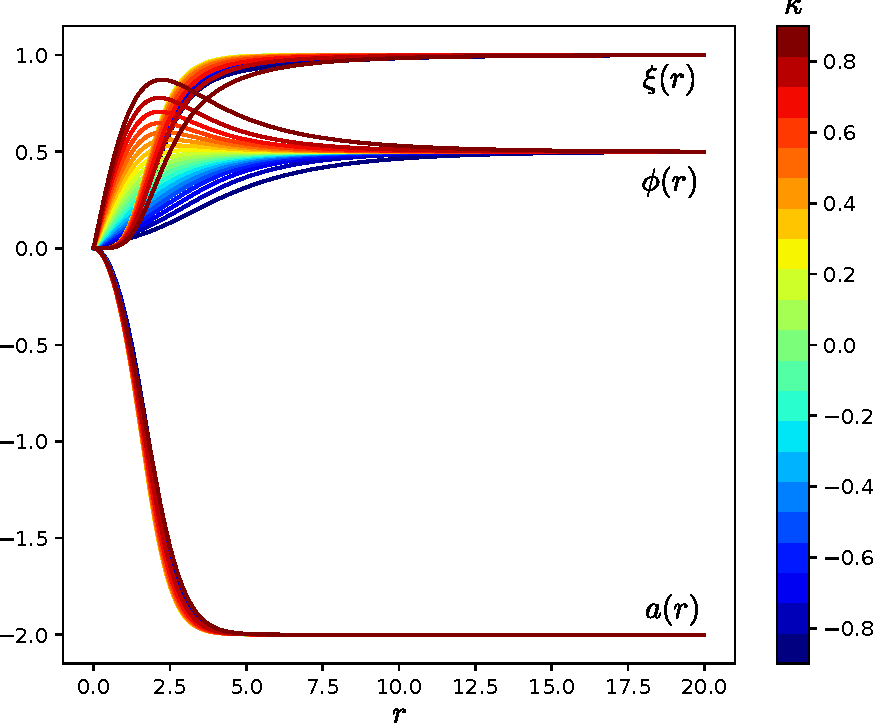
\includegraphics[scale=1]{./figures/F2.pdf}
	
	\caption{Solutions for the cosmic string profile functions with $v = 0.5$, $v'=1$, $n=1$, $n'=-5$, $h=0.5$, $h'=-2.5$, $\lambda=\lambda'=1$. This represents another example within the SO(10) GUT model. The overshoot of the field $\phi$ is clearly visible. Around $r=0$ the field $\xi$ is flat since in this region the solution is proportional to $r^{|n'|}$.}
	\label{fig:fig5}
\end{figure}

\begin{figure}
	\centering
	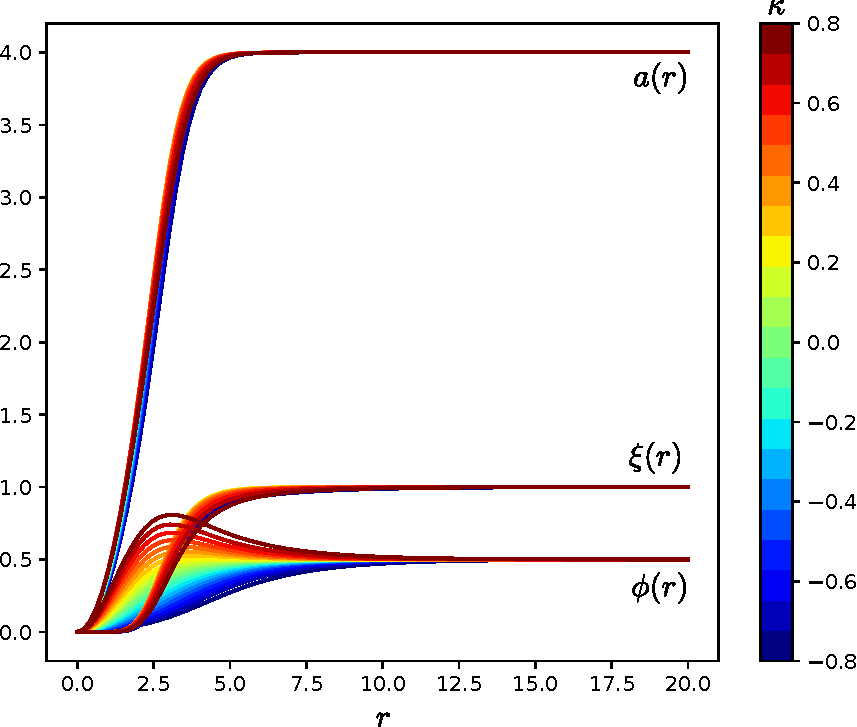
\includegraphics[scale=1]{./figures/F3.pdf}
	\caption{Solutions for the cosmic string profile functions with $v = 0.5$, $v'=1$, $n=-2$, $n'=10$, $h=0.5$, $h'=-2.5$, $\lambda=\lambda'=1$. This is another example within the SO(10) model. The overshoot of the field $\phi$ is clearly visible. Around $r=0$ the field $\xi$ is flatter than the previous case since the solution is proportional to $r^{|n'|}$.}
	\label{fig:fig6}
\end{figure}

%\begin{figure}
%	\centering
%	\begin{tikzpicture}[spy using outlines={magnification = 6, circle, size=6cm,black,connect spies}]	
%	\node (n1) at (0,0) {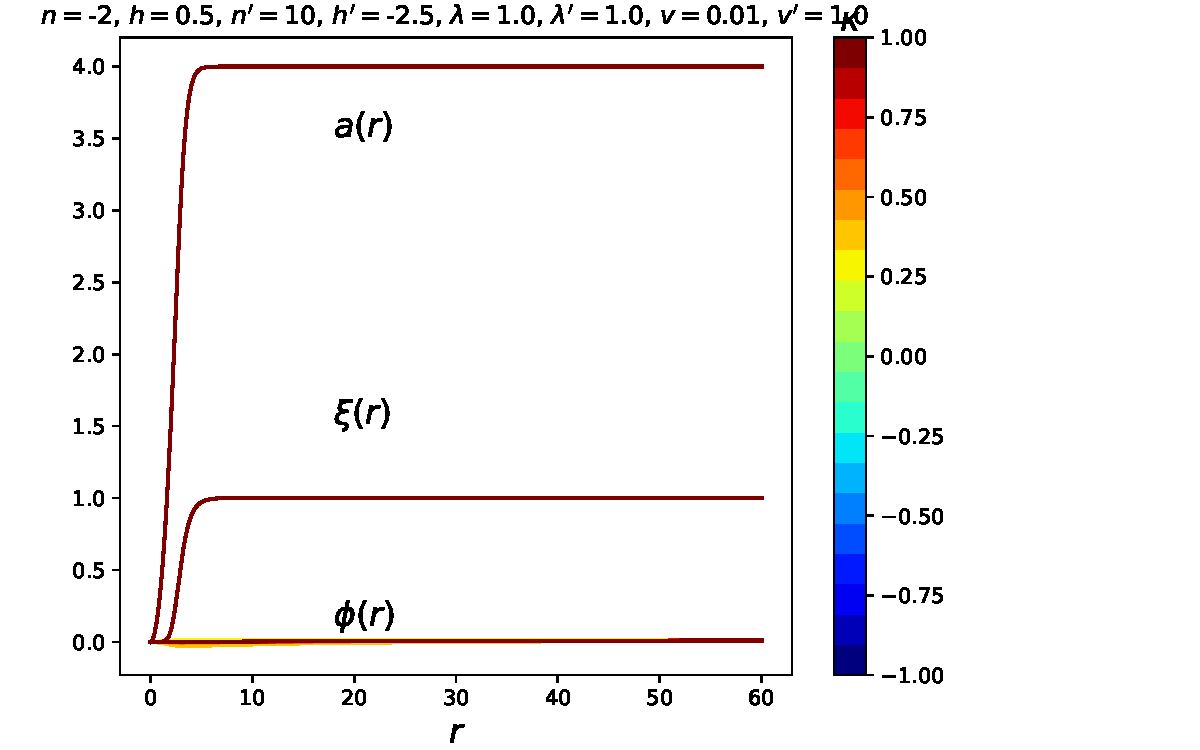
\includegraphics[scale=1]{./figures/n-2h05np10hp-25l1lp1v001vp1.pdf}};
%	\spy on (-7,-4.5) in node at (0,1);
%	\end{tikzpicture}
%\end{figure}

%\begin{figure}
%	\centering
%	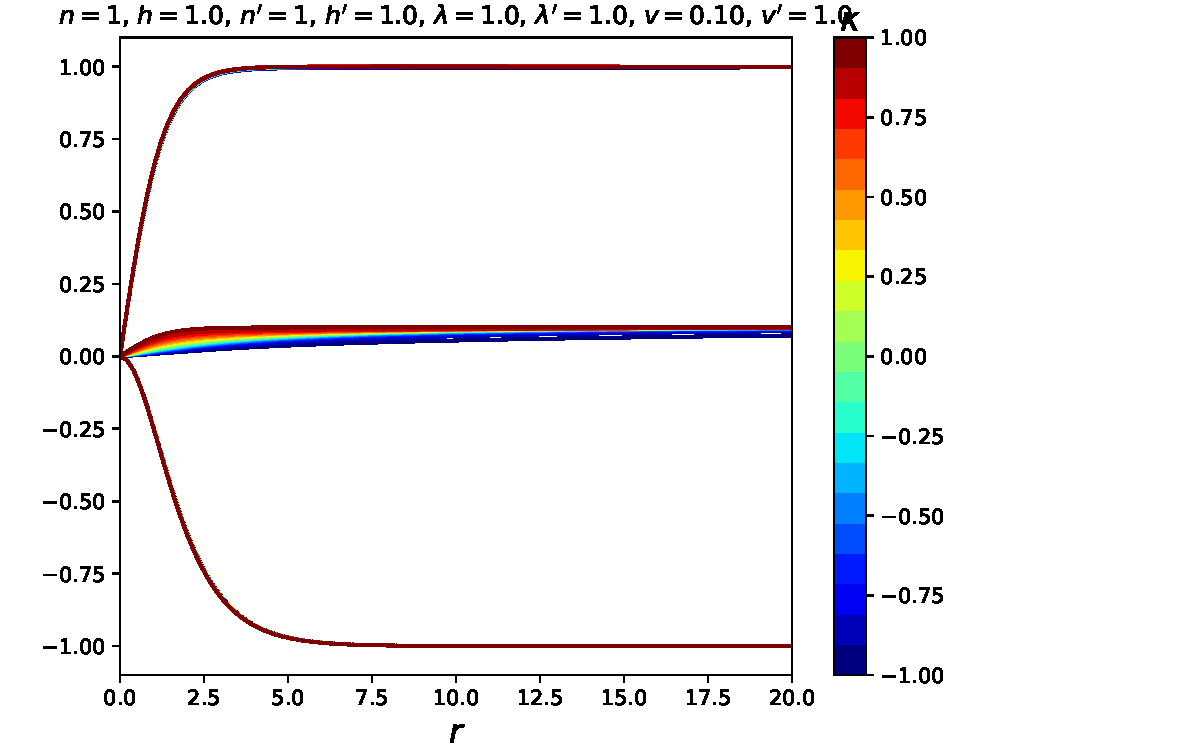
\includegraphics[scale=1]{./figures/n1h1np1hp1l1lp1v01vp1.pdf}
%	\caption{Solutions for the cosmic string profile functions with $v = 0.01$, $v'=1$, $n=-2$, $n'=10$, $h=0.5$, $h'=-2.5$, $\lambda=\lambda'=1$. Coaxial string solutions are found in a range with $\kappa>0$. A possible interpretation of the coaxial solutions regards the instability of such string with a high winding number.}
%	\label{fig:coaxial}
%\end{figure}
%
%
%\begin{figure}
%	\centering
%	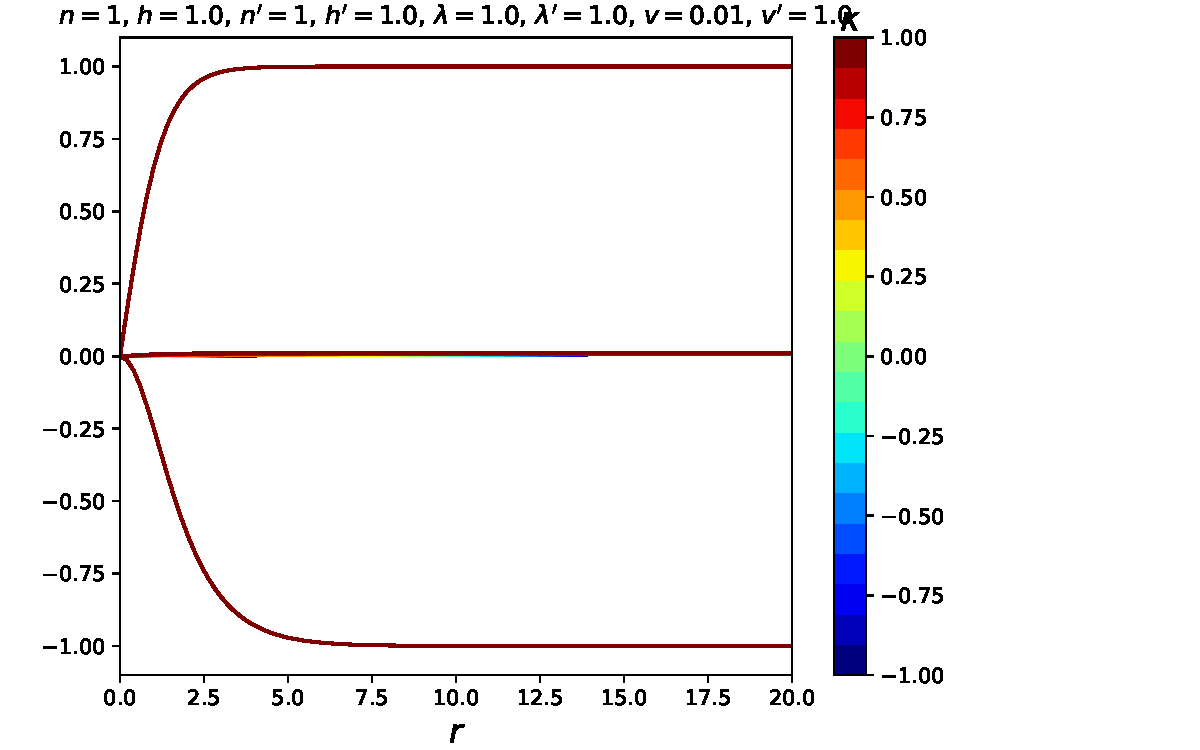
\includegraphics[scale=1]{./figures/n1h1np1hp1l1lp1v001vp1.pdf}
%	\caption{Solutions for the cosmic string profile functions with $v = 0.01$, $v'=1$, $n=-2$, $n'=10$, $h=0.5$, $h'=-2.5$, $\lambda=\lambda'=1$. Coaxial string solutions are found in a range with $\kappa>0$.}
%	\label{fig:coaxial}
%\end{figure}

\begin{figure}
	\centering
	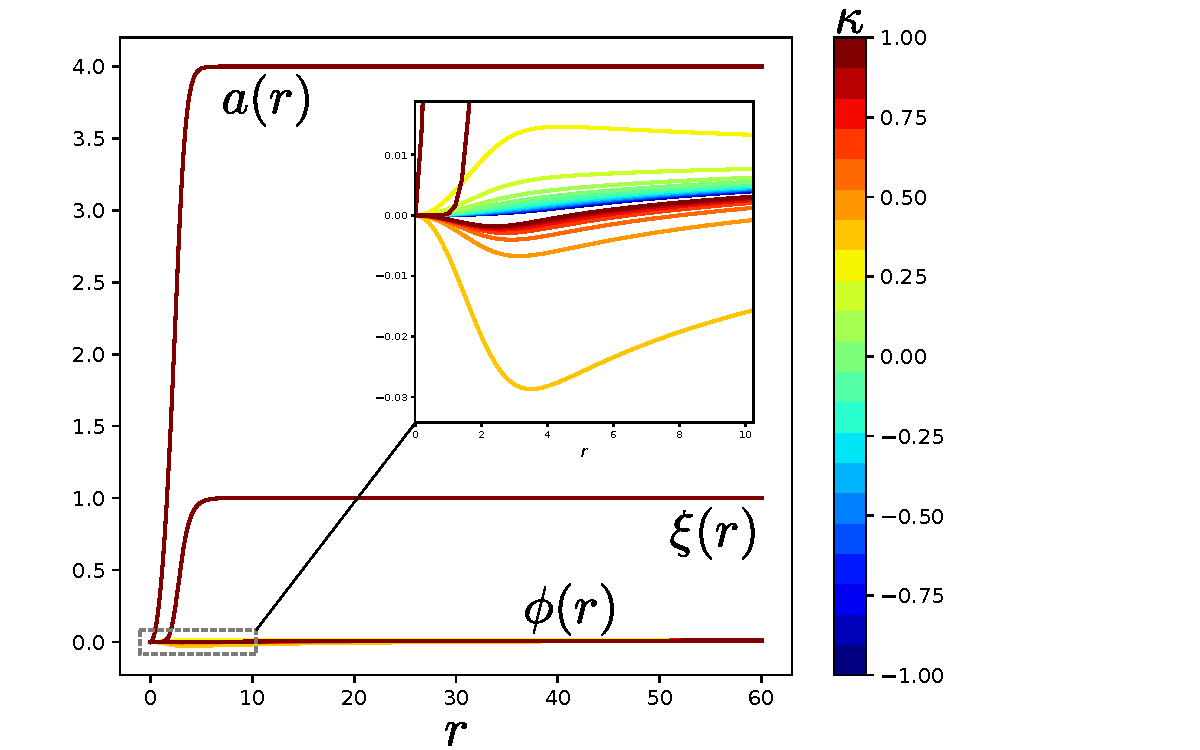
\includegraphics[scale=1]{./figures/n-2h05np10hp-25l1lp1v001vp1combined.pdf}
	\caption{Solutions for the cosmic string profile functions with $v = 0.01$, $v'=1$, $n=-2$, $n'=10$, $h=0.5$, $h'=-2.5$, $\lambda=\lambda'=1$. Coaxial string solutions are found in a range with $\kappa>0$.}
	\label{fig:coaxial}
\end{figure}

\begin{figure}
	\centering
	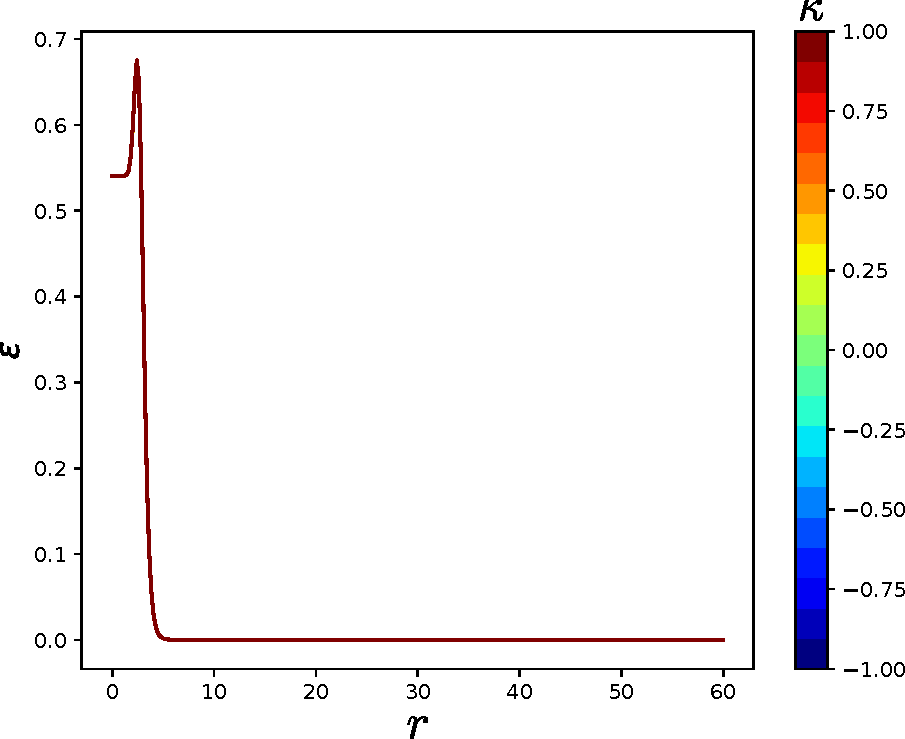
\includegraphics[scale=1]{./figures/n-2h05np10hp-25l1lp1v001vp1eden.pdf}
	\caption{Energy density of the solutions for the cosmic string profile functions with $v = 0.01$, $v'=1$, $n=-2$, $n'=10$, $h=0.5$, $h'=-2.5$, $\lambda=\lambda'=1$. The energy density is given in units of $4.79\times 10^{19}\ \text{GeV}/\text{fm}^3$.}
	\label{fig:edencoaxial}
\end{figure}

%\begin{figure}
%	\centering
%	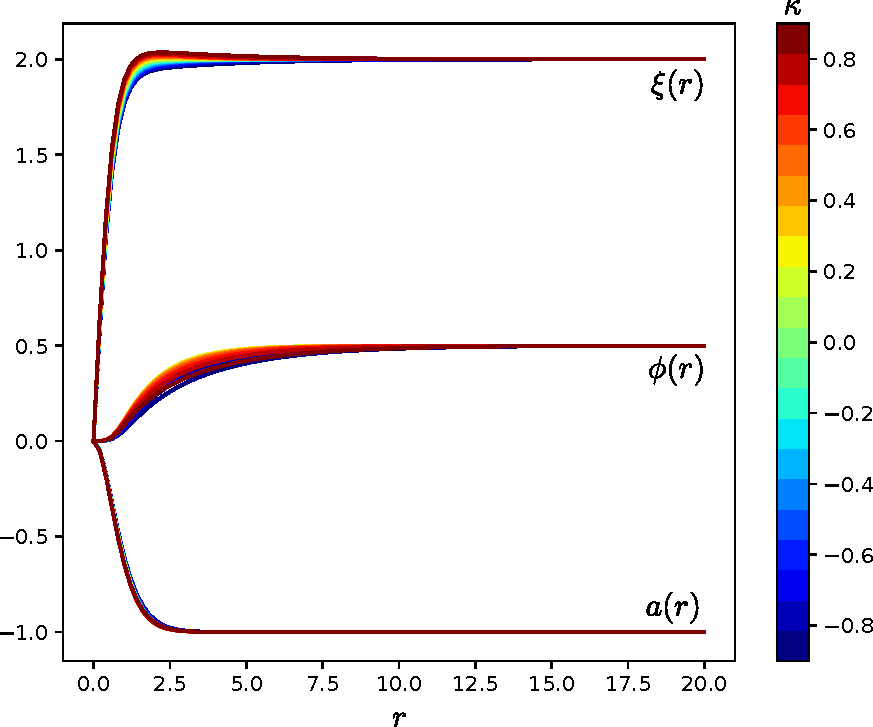
\includegraphics[scale=1]{./figures/n5h5np1hp1l1lp1v05v2.pdf}
%	\caption{Solutions for the cosmic string profile functions with $v = 0.5$, $v'=2$, $n=5$, $n'=1$, $h=5$, $h'=1$, $\lambda=\lambda'=1$.}
%	\label{fig:n5h5np1hp1l1lp1v05v2}
%\end{figure}
%
%\begin{figure}
%	\centering
%	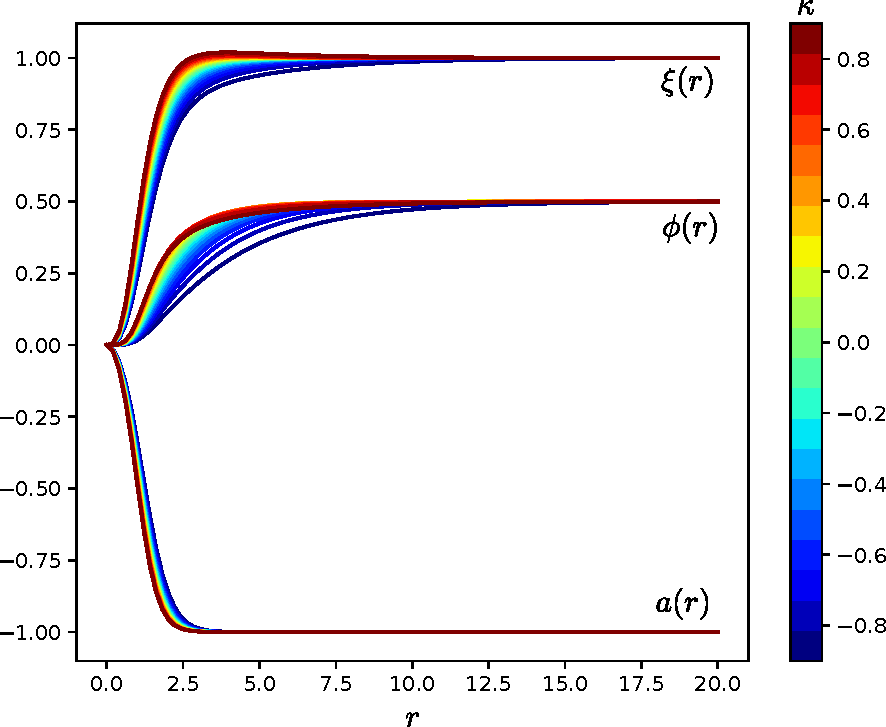
\includegraphics[scale=1]{./figures/n5h5np3h3l1lp1v05vp1.pdf}
%	\caption{Solutions for the cosmic string profile functions with $v = 0.5$, $v'=1$, $n=5$, $n'=3$, $h=5$, $h'=3$, $\lambda=\lambda'=1$.}
%	\label{fig:n5h5np3hp3l1lp1v05vp1}
%\end{figure}
%
%\begin{figure}
%	\centering
%	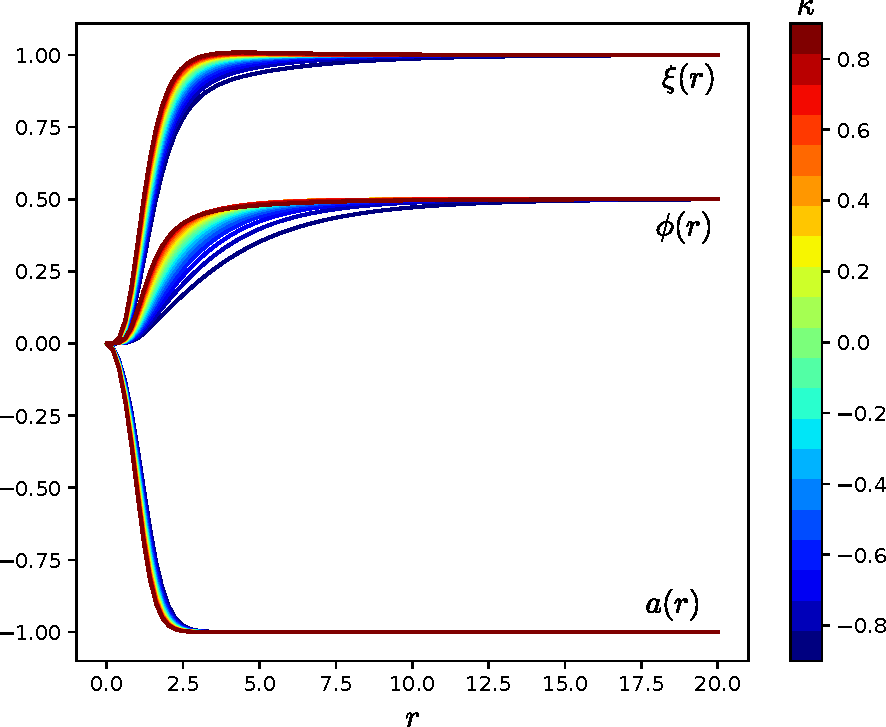
\includegraphics[scale=1]{./figures/n5h5np4hp4l1lp1v05vp1.pdf}
%	\caption{Solutions for the cosmic string profile functions with $v = 0.5$, $v'=1$, $n=5$, $n'=4$, $h=5$, $h'=4$, $\lambda=\lambda'=1$.}
%	\label{fig:n5h5np4hp4l1lp1v05vp1}
%\end{figure}



\chapter{Summary and conclusions}%U$(1)_{Y}\otimes$
In this thesis we have discussed an extension to the Standard Model by promoting the global U$(1)_{B-L}$ invariance to a local symmetry. We form a new hyper\-charge $Y'$, by taking a linear combination of the weak hypercharge $Y$, from the U$(1)_Y$ gauge symmetry, and the  difference between the baryon and lepton numbers $B-L$, from U$(1)_{B-L}$. Therefore, we introduced a new gauge coupling $h'$ that couples the Abelian gauge field to $B-L$.
The new charge $Y'$  is defined as
\begin{equation}
	Y' \equiv 2hY+\frac{h'}{2}(B-L),
\end{equation}
 where $h$ is the coupling to the weak hypercharge. Therefore, the new gauge group is U$(1)_{Y'}$.
 
This way, we converted the Standard Model symmetry group to
 \begin{equation}
	\text{SU}(3)\times \text{SU}(2)_L\times \text{U}(1)_{Y'}.
\end{equation}
 
The introduction of the new gauge coupling generates gauge anomalies, as seen in the triangular diagram in Figure \ref{fig:anomaly}. In order to remove the anomalies, we introduced a right-handed neutrino $\nu_R$ in each fermion genera\-tion. 
 %Therefore, we need the addition of three new fields, a gauge field $\mathcal{A}_{\mu}$ responsible for the local U$(1)_{Y'}$ symmetry, however, gauge anomalies arise, so we also added a right-handed neutrino $\nu_{R}$, and finally we added a new Higgs field $\chi$ in order to give mass to $\nu_{R}$.
We give mass to the neutrinos via the Higgs mechanism. However, if we want to give another mass to the right-handed neutrino, independently from the left-handed neutrino, the standard Majorana term is not applicable, so we introduce a new Higgs field $\chi\in \mathbb{C}$ and its vacuum expectation value $v'$. This new scalar field has a charge $B-L=-2$ in order to preserve gauge invariance. We also introduced a coupling term between the two Higgs fields, $\kappa \Phi^{\dagger}\Phi \chi^{*}\chi$, in the Lagrangian.

As a simplified model, we only considered the U$(1)_{Y'}$ as the gauge group. This model allows for vortex-line solutions or cosmic strings.
 
 We then studied the system of field equations for $\Phi$, $\chi$ and $\mathcal{A}_{\mu}$. We made cylindrical ansätze for these fields in order to study cosmic string solutions and solved the system of equations with appropriate boundary conditions at $r=0$ and $r\to\infty$.

We used $v=246 \ \text{GeV}$ to convert all quantities into physical units. For instance, in some plots of Chapter \ref{chap:results} we used $v=0.5$. This way, the typical length $r = 1$ is equal in physical units to $r = \frac{0.5}{246\ \text{GeV}}0.197\ \text{GeV}\ \text{fm}\approx 0.0004\ \text{fm}$.

We observed that the $\kappa$ value has a modest effect on the solutions for $a$ and $\xi$, but a significant effect on $\phi$, specially in the low $r$ regime.

Our contribution to the literature is the finding of co-axial and overshoot solutions. We found co-axial solutions for the field $\phi$ that are negative at low $r$, pass the $r$ axis, and then approach their positive vacuum expectation value. Surprisingly, we observed also the opposite effect: inside the string, depending on the values of the winding numbers, the fields $\Phi$ or $\chi$ can overshoot its vacuum expectation value. That is, the field can take a higher value than its VEV. The overshoot is more visible when considering the constraints form the SO(10) model, a Grand Unified Theory. Physically, we can interpret the overshoot as a temporarily increase in the mass of a near passing particle.

This modest but fully consistent extension of the Standard Model allows  for a non-standard type of cosmic strings. The tension of these kinds of strings is of the order of $10^{10}\ \text{MeV}^2$, and have a gravitational coupling near to $10^{-30}$.

The scenario of cosmic strings that we have studied seems realistic. The proposals for an observational test are slim, unfortunately. However, this also means that such cosmic strings are most likely not ruled out based on existing data. A valid argument in its favor is the original motivation of explaining why the $B-L$ invariance is an exact symmetry.



%\appendix
%\chapter{}

\bibliography{bibliography}


\end{document}